\documentclass[]{book}
\usepackage{lmodern}
\usepackage{amssymb,amsmath}
\usepackage{ifxetex,ifluatex}
\usepackage{fixltx2e} % provides \textsubscript
\ifnum 0\ifxetex 1\fi\ifluatex 1\fi=0 % if pdftex
  \usepackage[T1]{fontenc}
  \usepackage[utf8]{inputenc}
\else % if luatex or xelatex
  \ifxetex
    \usepackage{mathspec}
  \else
    \usepackage{fontspec}
  \fi
  \defaultfontfeatures{Ligatures=TeX,Scale=MatchLowercase}
\fi
% use upquote if available, for straight quotes in verbatim environments
\IfFileExists{upquote.sty}{\usepackage{upquote}}{}
% use microtype if available
\IfFileExists{microtype.sty}{%
\usepackage{microtype}
\UseMicrotypeSet[protrusion]{basicmath} % disable protrusion for tt fonts
}{}
\usepackage[margin=1in]{geometry}
\usepackage{hyperref}
\hypersetup{unicode=true,
            pdftitle={Lecture Note for Applied Econometrics},
            pdfauthor={Yuta Toyama},
            pdfborder={0 0 0},
            breaklinks=true}
\urlstyle{same}  % don't use monospace font for urls
\usepackage{color}
\usepackage{fancyvrb}
\newcommand{\VerbBar}{|}
\newcommand{\VERB}{\Verb[commandchars=\\\{\}]}
\DefineVerbatimEnvironment{Highlighting}{Verbatim}{commandchars=\\\{\}}
% Add ',fontsize=\small' for more characters per line
\usepackage{framed}
\definecolor{shadecolor}{RGB}{248,248,248}
\newenvironment{Shaded}{\begin{snugshade}}{\end{snugshade}}
\newcommand{\KeywordTok}[1]{\textcolor[rgb]{0.13,0.29,0.53}{\textbf{#1}}}
\newcommand{\DataTypeTok}[1]{\textcolor[rgb]{0.13,0.29,0.53}{#1}}
\newcommand{\DecValTok}[1]{\textcolor[rgb]{0.00,0.00,0.81}{#1}}
\newcommand{\BaseNTok}[1]{\textcolor[rgb]{0.00,0.00,0.81}{#1}}
\newcommand{\FloatTok}[1]{\textcolor[rgb]{0.00,0.00,0.81}{#1}}
\newcommand{\ConstantTok}[1]{\textcolor[rgb]{0.00,0.00,0.00}{#1}}
\newcommand{\CharTok}[1]{\textcolor[rgb]{0.31,0.60,0.02}{#1}}
\newcommand{\SpecialCharTok}[1]{\textcolor[rgb]{0.00,0.00,0.00}{#1}}
\newcommand{\StringTok}[1]{\textcolor[rgb]{0.31,0.60,0.02}{#1}}
\newcommand{\VerbatimStringTok}[1]{\textcolor[rgb]{0.31,0.60,0.02}{#1}}
\newcommand{\SpecialStringTok}[1]{\textcolor[rgb]{0.31,0.60,0.02}{#1}}
\newcommand{\ImportTok}[1]{#1}
\newcommand{\CommentTok}[1]{\textcolor[rgb]{0.56,0.35,0.01}{\textit{#1}}}
\newcommand{\DocumentationTok}[1]{\textcolor[rgb]{0.56,0.35,0.01}{\textbf{\textit{#1}}}}
\newcommand{\AnnotationTok}[1]{\textcolor[rgb]{0.56,0.35,0.01}{\textbf{\textit{#1}}}}
\newcommand{\CommentVarTok}[1]{\textcolor[rgb]{0.56,0.35,0.01}{\textbf{\textit{#1}}}}
\newcommand{\OtherTok}[1]{\textcolor[rgb]{0.56,0.35,0.01}{#1}}
\newcommand{\FunctionTok}[1]{\textcolor[rgb]{0.00,0.00,0.00}{#1}}
\newcommand{\VariableTok}[1]{\textcolor[rgb]{0.00,0.00,0.00}{#1}}
\newcommand{\ControlFlowTok}[1]{\textcolor[rgb]{0.13,0.29,0.53}{\textbf{#1}}}
\newcommand{\OperatorTok}[1]{\textcolor[rgb]{0.81,0.36,0.00}{\textbf{#1}}}
\newcommand{\BuiltInTok}[1]{#1}
\newcommand{\ExtensionTok}[1]{#1}
\newcommand{\PreprocessorTok}[1]{\textcolor[rgb]{0.56,0.35,0.01}{\textit{#1}}}
\newcommand{\AttributeTok}[1]{\textcolor[rgb]{0.77,0.63,0.00}{#1}}
\newcommand{\RegionMarkerTok}[1]{#1}
\newcommand{\InformationTok}[1]{\textcolor[rgb]{0.56,0.35,0.01}{\textbf{\textit{#1}}}}
\newcommand{\WarningTok}[1]{\textcolor[rgb]{0.56,0.35,0.01}{\textbf{\textit{#1}}}}
\newcommand{\AlertTok}[1]{\textcolor[rgb]{0.94,0.16,0.16}{#1}}
\newcommand{\ErrorTok}[1]{\textcolor[rgb]{0.64,0.00,0.00}{\textbf{#1}}}
\newcommand{\NormalTok}[1]{#1}
\usepackage{longtable,booktabs}
\usepackage{graphicx,grffile}
\makeatletter
\def\maxwidth{\ifdim\Gin@nat@width>\linewidth\linewidth\else\Gin@nat@width\fi}
\def\maxheight{\ifdim\Gin@nat@height>\textheight\textheight\else\Gin@nat@height\fi}
\makeatother
% Scale images if necessary, so that they will not overflow the page
% margins by default, and it is still possible to overwrite the defaults
% using explicit options in \includegraphics[width, height, ...]{}
\setkeys{Gin}{width=\maxwidth,height=\maxheight,keepaspectratio}
\IfFileExists{parskip.sty}{%
\usepackage{parskip}
}{% else
\setlength{\parindent}{0pt}
\setlength{\parskip}{6pt plus 2pt minus 1pt}
}
\setlength{\emergencystretch}{3em}  % prevent overfull lines
\providecommand{\tightlist}{%
  \setlength{\itemsep}{0pt}\setlength{\parskip}{0pt}}
\setcounter{secnumdepth}{5}
% Redefines (sub)paragraphs to behave more like sections
\ifx\paragraph\undefined\else
\let\oldparagraph\paragraph
\renewcommand{\paragraph}[1]{\oldparagraph{#1}\mbox{}}
\fi
\ifx\subparagraph\undefined\else
\let\oldsubparagraph\subparagraph
\renewcommand{\subparagraph}[1]{\oldsubparagraph{#1}\mbox{}}
\fi

%%% Use protect on footnotes to avoid problems with footnotes in titles
\let\rmarkdownfootnote\footnote%
\def\footnote{\protect\rmarkdownfootnote}

%%% Change title format to be more compact
\usepackage{titling}

% Create subtitle command for use in maketitle
\newcommand{\subtitle}[1]{
  \posttitle{
    \begin{center}\large#1\end{center}
    }
}

\setlength{\droptitle}{-2em}

  \title{Lecture Note for Applied Econometrics}
    \pretitle{\vspace{\droptitle}\centering\huge}
  \posttitle{\par}
    \author{Yuta Toyama}
    \preauthor{\centering\large\emph}
  \postauthor{\par}
      \predate{\centering\large\emph}
  \postdate{\par}
    \date{Last updated: 2019/06/03}


\begin{document}
\maketitle

{
\setcounter{tocdepth}{1}
\tableofcontents
}
\chapter{Preface}\label{preface}

Welcome to Applied Econometrics using R!

\section{About this}\label{about-this}

This lecture note is maintained by Yuta Toyama.

\section{Update: April 23, 2019}\label{update-april-23-2019}

\begin{itemize}
\tightlist
\item
  Upload chapter 6 (review of statistics)
\end{itemize}

\section{Update: April 16, 2019}\label{update-april-16-2019}

\begin{itemize}
\tightlist
\item
  Update chapter 3 (basic programming)
\item
  Upload chapter 4 (Data frame)
\item
  Upload chapter 5 (Exercise 1)
\end{itemize}

\section{Acknowledgement (as of April 16,
2019)}\label{acknowledgement-as-of-april-16-2019}

\begin{itemize}
\tightlist
\item
  Chapter 2 through 4 are largely based on Applied Statistics with
  \texttt{R}. \url{https://daviddalpiaz.github.io/appliedstats/}
\item
  Chapter 6 is based on ``Introduction to Econometrics with R''.
  \url{https://www.econometrics-with-r.org/index.html}
\end{itemize}

\chapter{Introduction to the course}\label{introduction-to-the-course}

\section{What is econometrics?}\label{what-is-econometrics}

\begin{enumerate}
\def\labelenumi{\arabic{enumi}.}
\tightlist
\item
  Estimating economic relationships

  \begin{enumerate}
  \def\labelenumii{\arabic{enumii}.}
  \tightlist
  \item
    Demand curve \(\log(Q_{t})= \alpha_0 + \alpha_1 P_t + \epsilon_t\)
  \item
    Production function \(Y_{it}=A_{it}K_{it}^{\alpha}L_{it}^{\beta}\)
  \end{enumerate}
\item
  Testing economic theory

  \begin{itemize}
  \tightlist
  \item
    Does adverse selection exists in insurance markets?
  \item
    Are consumers rational?
  \end{itemize}
\item
  Determine the effect of a given intervention (causal inference)

  \begin{itemize}
  \tightlist
  \item
    What is the effect of increasing minimum wage on employment?
  \item
    Do mergers increase the output price?
  \item
    Does democracy cause economic growth? (a series of works by
    Acemoglu, Robinsohn, and their co-authors).
  \item
    Effects of going to private colleges on your future earnings.
  \item
    Note: Some questions may have underlying economic models, others may
    not.
  \end{itemize}
\item
  Describe the data (prediction/forecasting)

  \begin{itemize}
  \tightlist
  \item
    How does the distribution of wage look like?
  \item
    Relationship between electricity consumption and temperature
    (possibly nonlinear).
  \item
    Related to machine learning (ML).
  \end{itemize}
\end{enumerate}

\section{Why do we need to learn
computation}\label{why-do-we-need-to-learn-computation}

\begin{enumerate}
\def\labelenumi{\arabic{enumi}.}
\tightlist
\item
  Conduct statistical and empirical analysis using your own data set

  \begin{enumerate}
  \def\labelenumii{\arabic{enumii}.}
  \tightlist
  \item
    Construct the data set
  \item
    Describe the data
  \item
    Run regression or estimate an economic object
  \item
    Make tables and figures that show the results of your analysis.
  \end{enumerate}
\item
  Verify the econometric theory through numerical simulations.

  \begin{itemize}
  \tightlist
  \item
    Ex. Asymptotic theory considers the case when the sample size is
    large enough (i.e., \(N \rightarrow \infty\))

    \begin{itemize}
    \tightlist
    \item
      Law of large numbers, central limit theorem
    \item
      How well is the asymptotic approximation?
    \end{itemize}
  \item
    \textbf{Monte Carlo simulations}
  \end{itemize}
\end{enumerate}

\begin{itemize}
\tightlist
\item
  We will learn both aspects in this course.
\end{itemize}

\section{Why do we use R?}\label{why-do-we-use-r}

\begin{itemize}
\tightlist
\item
  Many alternatives: Stata, Matlab, Python, etc\ldots{}
\end{itemize}

\begin{enumerate}
\def\labelenumi{\arabic{enumi}.}
\tightlist
\item
  Free software!!

  \begin{itemize}
  \tightlist
  \item
    Stata and Matlab are expensive.
  \item
    Though you can use Matlab through the campus license from this
    April.
  \end{itemize}
\item
  Good balance between flexibility in programming and easy-to-use for
  econometric analysis

  \begin{itemize}
  \tightlist
  \item
    Stata is easy to use for econometric analysis, but hard to write
    your own program.
  \item
    Matlab is the opposite.
  \item
    You can do everything with R, including data construction,
    regression analysis, and complicated structural estimation.
  \end{itemize}
\item
  Many users

  \begin{itemize}
  \tightlist
  \item
    Popular in engineering.
  \item
    Many packages being developed (especially important for recently
    popular tools. )
  \end{itemize}
\end{enumerate}

\begin{itemize}
\tightlist
\item
  Note: Python seems also good, though I have not used it before.
\end{itemize}

\chapter{\texorpdfstring{Introduction of \texttt{R} and
\texttt{R\ studio}}{Introduction of R and R studio}}\label{introduction-of-r-and-r-studio}

\section{Getting Started}\label{getting-started}

\begin{itemize}
\tightlist
\item
  You can use R/R studio in the PC room.
\item
  However, I strongly recommend you install R/Studio in your laptop and
  bring it to the class.
\item
  Install in the following order

  \begin{enumerate}
  \def\labelenumi{\arabic{enumi}.}
  \tightlist
  \item
    R: \url{https://www.r-project.org/}
  \item
    Rstudio: \url{https://www.rstudio.com/}
  \end{enumerate}
\item
  Now open Rstudio.
\end{itemize}

\section{Helps}\label{helps}

\begin{itemize}
\tightlist
\item
  The RStudio team has developed
  \href{https://www.rstudio.com/resources/cheatsheets/}{a number of
  ``cheatsheets''} for working with both \texttt{R} and RStudio.
\item
  \href{http://www.rstudio.com/wp-content/uploads/2016/05/base-r.pdf}{This
  particular cheatsheet for Base \texttt{R}} will summarize many of the
  concepts in this document.
\end{itemize}

\section{Quick tour of Rstudio}\label{quick-tour-of-rstudio}

\begin{itemize}
\tightlist
\item
  There are four panels

  \begin{enumerate}
  \def\labelenumi{\arabic{enumi}.}
  \tightlist
  \item
    Source: Write your own code here.
  \item
    Console:
  \item
    Environment/History:
  \item
    Files/Plots/Packages/Help:
  \end{enumerate}
\item
  In the Source panel,

  \begin{itemize}
  \tightlist
  \item
    Write your own code.
  \item
    Save your code in \texttt{.R} file
  \item
    Click \texttt{Run} command to run your entire code.
  \end{itemize}
\item
  In the concole panel,

  \begin{itemize}
  \tightlist
  \item
    After clicking \texttt{Run} in the source panel, your code is
    evaluated.
  \item
    You can directly type your code here to implement.
  \end{itemize}
\end{itemize}

\section{Basic Calculations}\label{basic-calculations}

To get started, we'll use \texttt{R} like a simple calculator.

\subsubsection*{Addition, Subtraction, Multiplication and
Division}\label{addition-subtraction-multiplication-and-division}
\addcontentsline{toc}{subsubsection}{Addition, Subtraction,
Multiplication and Division}

\begin{longtable}[]{@{}lll@{}}
\toprule
Math & \texttt{R} & Result\tabularnewline
\midrule
\endhead
\(3 + 2\) & \texttt{3\ +\ 2} & 5\tabularnewline
\(3 - 2\) & \texttt{3\ -\ 2} & 1\tabularnewline
\(3 \cdot2\) & \texttt{3\ *\ 2} & 6\tabularnewline
\(3 / 2\) & \texttt{3\ /\ 2} & 1.5\tabularnewline
\bottomrule
\end{longtable}

\subsubsection*{Exponents}\label{exponents}
\addcontentsline{toc}{subsubsection}{Exponents}

\begin{longtable}[]{@{}lll@{}}
\toprule
Math & \texttt{R} & Result\tabularnewline
\midrule
\endhead
\(3^2\) & \texttt{3\ \^{}\ 2} & 9\tabularnewline
\(2^{(-3)}\) & \texttt{2\ \^{}\ (-3)} & 0.125\tabularnewline
\(100^{1/2}\) & \texttt{100\ \^{}\ (1\ /\ 2)} & 10\tabularnewline
\(\sqrt{100}\) & \texttt{sqrt(100)} & 10\tabularnewline
\bottomrule
\end{longtable}

\subsubsection*{Mathematical Constants}\label{mathematical-constants}
\addcontentsline{toc}{subsubsection}{Mathematical Constants}

\begin{longtable}[]{@{}lll@{}}
\toprule
Math & \texttt{R} & Result\tabularnewline
\midrule
\endhead
\(\pi\) & \texttt{pi} & 3.1415927\tabularnewline
\(e\) & \texttt{exp(1)} & 2.7182818\tabularnewline
\bottomrule
\end{longtable}

\subsubsection*{Logarithms}\label{logarithms}
\addcontentsline{toc}{subsubsection}{Logarithms}

\begin{itemize}
\tightlist
\item
  Note that we will use \(\ln\) and \(\log\) interchangeably to mean the
  natural logarithm.
\item
  There is no \texttt{ln()} in \texttt{R}, instead it uses
  \texttt{log()} to mean the natural logarithm.
\end{itemize}

\begin{longtable}[]{@{}lll@{}}
\toprule
Math & \texttt{R} & Result\tabularnewline
\midrule
\endhead
\(\log(e)\) & \texttt{log(exp(1))} & 1\tabularnewline
\(\log_{10}(1000)\) & \texttt{log10(1000)} & 3\tabularnewline
\(\log_{2}(8)\) & \texttt{log2(8)} & 3\tabularnewline
\(\log_{4}(16)\) & \texttt{log(16,\ base\ =\ 4)} & 2\tabularnewline
\bottomrule
\end{longtable}

\subsubsection*{Trigonometry}\label{trigonometry}
\addcontentsline{toc}{subsubsection}{Trigonometry}

\begin{longtable}[]{@{}lll@{}}
\toprule
Math & \texttt{R} & Result\tabularnewline
\midrule
\endhead
\(\sin(\pi / 2)\) & \texttt{sin(pi\ /\ 2)} & 1\tabularnewline
\(\cos(0)\) & \texttt{cos(0)} & 1\tabularnewline
\bottomrule
\end{longtable}

\section{Getting Help}\label{getting-help}

\begin{itemize}
\tightlist
\item
  In using \texttt{R} as a calculator, we have seen a number of
  functions: \texttt{sqrt()}, \texttt{exp()}, \texttt{log()} and
  \texttt{sin()}.
\item
  To get documentation about a function in \texttt{R}, simply put a
  question mark in front of the function name and RStudio will display
  the documentation, for example:
\end{itemize}

\begin{Shaded}
\begin{Highlighting}[]
\NormalTok{?log}
\NormalTok{?sin}
\NormalTok{?paste}
\NormalTok{?lm}
\end{Highlighting}
\end{Shaded}

\section{Installing Packages}\label{installing-packages}

\begin{itemize}
\tightlist
\item
  One of the main strengths of \texttt{R} as an open-source project is
  its package system.
\item
  To install a package, use the \texttt{install.packages()} function.

  \begin{itemize}
  \tightlist
  \item
    Think of this as buying a recipe book from the store, bringing it
    home, and putting it on your shelf.
  \end{itemize}
\end{itemize}

\begin{Shaded}
\begin{Highlighting}[]
\KeywordTok{install.packages}\NormalTok{(}\StringTok{"ggplot2"}\NormalTok{)}
\end{Highlighting}
\end{Shaded}

\begin{itemize}
\tightlist
\item
  Once a package is installed, it must be loaded into your current
  \texttt{R} session before being used.

  \begin{itemize}
  \tightlist
  \item
    Think of this as taking the book off of the shelf and opening it up
    to read.
  \end{itemize}
\end{itemize}

\begin{Shaded}
\begin{Highlighting}[]
\KeywordTok{library}\NormalTok{(ggplot2)}
\end{Highlighting}
\end{Shaded}

\begin{itemize}
\tightlist
\item
  Once you close \texttt{R}, all the packages are closed and put back on
  the imaginary shelf.
\item
  The next time you open \texttt{R}, you do not have to install the
  package again, but you do have to load any packages you intend to use
  by invoking \texttt{library()}.
\end{itemize}

\chapter{Data and Programming}\label{data-and-programming}

\section{Data Types}\label{data-types}

\texttt{R} has a number of basic data \emph{types}.

\begin{itemize}
\tightlist
\item
  Numeric

  \begin{itemize}
  \tightlist
  \item
    Also known as Double. The default type when dealing with numbers.
  \item
    Examples: \texttt{1}, \texttt{1.0}, \texttt{42.5}
  \end{itemize}
\item
  Logical

  \begin{itemize}
  \tightlist
  \item
    Two possible values: \texttt{TRUE} and \texttt{FALSE}
  \item
    You can also use \texttt{T} and \texttt{F}, but this is \emph{not}
    recommended.
  \item
    \texttt{NA} is also considered logical.
  \end{itemize}
\item
  Character

  \begin{itemize}
  \tightlist
  \item
    Examples: \texttt{"a"}, \texttt{"Statistics"},
    \texttt{"1\ plus\ 2."}
  \end{itemize}
\end{itemize}

\section{Data Structures}\label{data-structures}

\begin{itemize}
\tightlist
\item
  \texttt{R} also has a number of basic data \emph{structures}.
\item
  A data structure is either

  \begin{itemize}
  \tightlist
  \item
    homogeneous (all elements are of the same data type)
  \item
    heterogeneous (elements can be of more than one data type).
  \end{itemize}
\end{itemize}

\begin{longtable}[]{@{}lll@{}}
\toprule
Dimension & \textbf{Homogeneous} & \textbf{Heterogeneous}\tabularnewline
\midrule
\endhead
1 & Vector & List\tabularnewline
2 & Matrix & Data Frame\tabularnewline
3+ & Array &\tabularnewline
\bottomrule
\end{longtable}

\section{Vectors}\label{vectors}

\subsection{Basics of vectors}\label{basics-of-vectors}

\begin{itemize}
\tightlist
\item
  Many operations in \texttt{R} make heavy use of \textbf{vectors}.

  \begin{itemize}
  \tightlist
  \item
    Vectors in \texttt{R} are indexed starting at \texttt{1}.
  \end{itemize}
\item
  The most common way to create a vector in \texttt{R} is using the
  \texttt{c()} function, which is short for ``combine.''"
\end{itemize}

\begin{Shaded}
\begin{Highlighting}[]
\KeywordTok{c}\NormalTok{(}\DecValTok{1}\NormalTok{, }\DecValTok{3}\NormalTok{, }\DecValTok{5}\NormalTok{, }\DecValTok{7}\NormalTok{, }\DecValTok{8}\NormalTok{, }\DecValTok{9}\NormalTok{)}
\end{Highlighting}
\end{Shaded}

\begin{verbatim}
## [1] 1 3 5 7 8 9
\end{verbatim}

\begin{itemize}
\tightlist
\item
  If we would like to store this vector in a \textbf{variable} we can do
  so with the \textbf{assignment} operator \texttt{=}.

  \begin{itemize}
  \tightlist
  \item
    The variable \texttt{x} now holds the vector we just created, and we
    can access the vector by typing \texttt{x}.
  \end{itemize}
\end{itemize}

\begin{Shaded}
\begin{Highlighting}[]
\NormalTok{x =}\StringTok{ }\KeywordTok{c}\NormalTok{(}\DecValTok{1}\NormalTok{, }\DecValTok{3}\NormalTok{, }\DecValTok{5}\NormalTok{, }\DecValTok{7}\NormalTok{, }\DecValTok{8}\NormalTok{, }\DecValTok{9}\NormalTok{)}
\NormalTok{x}
\end{Highlighting}
\end{Shaded}

\begin{verbatim}
## [1] 1 3 5 7 8 9
\end{verbatim}

\begin{Shaded}
\begin{Highlighting}[]
\CommentTok{# The following does the same thing.}
\NormalTok{x <-}\StringTok{ }\KeywordTok{c}\NormalTok{(}\DecValTok{1}\NormalTok{, }\DecValTok{3}\NormalTok{, }\DecValTok{5}\NormalTok{, }\DecValTok{7}\NormalTok{, }\DecValTok{8}\NormalTok{, }\DecValTok{9}\NormalTok{)}
\NormalTok{x}
\end{Highlighting}
\end{Shaded}

\begin{verbatim}
## [1] 1 3 5 7 8 9
\end{verbatim}

\begin{itemize}
\tightlist
\item
  The operator \texttt{=} and \texttt{\textless{}-} work as an
  assignment operator.

  \begin{itemize}
  \tightlist
  \item
    You can use both. This does not matter usually.
  \item
    If you are interested in the weird cases where the difference
    matters, check out
    \href{http://www.burns-stat.com/documents/books/the-r-inferno/}{The
    R Inferno}.
  \end{itemize}
\item
  In \texttt{R} code the line starting with \texttt{\#} is
  \texttt{comment}, which is ignored when you run the fode.
\end{itemize}

\begin{itemize}
\tightlist
\item
  A vector based on a sequence of numbers.
\item
  The quickest and easiest way to do this is with the \texttt{:}
  operator, which creates a sequence of integers between two specified
  integers.
\end{itemize}

\begin{Shaded}
\begin{Highlighting}[]
\NormalTok{(}\DataTypeTok{y =} \DecValTok{1}\OperatorTok{:}\DecValTok{100}\NormalTok{)}
\end{Highlighting}
\end{Shaded}

\begin{verbatim}
##   [1]   1   2   3   4   5   6   7   8   9  10  11  12  13  14  15  16  17
##  [18]  18  19  20  21  22  23  24  25  26  27  28  29  30  31  32  33  34
##  [35]  35  36  37  38  39  40  41  42  43  44  45  46  47  48  49  50  51
##  [52]  52  53  54  55  56  57  58  59  60  61  62  63  64  65  66  67  68
##  [69]  69  70  71  72  73  74  75  76  77  78  79  80  81  82  83  84  85
##  [86]  86  87  88  89  90  91  92  93  94  95  96  97  98  99 100
\end{verbatim}

\begin{itemize}
\tightlist
\item
  By putting parentheses around the assignment,

  \begin{itemize}
  \tightlist
  \item
    \texttt{R} both stores the vector in a variable called \texttt{y}
    and
  \item
    automatically outputs \texttt{y} to the console.
  \end{itemize}
\end{itemize}

\subsection{Useful functions for creating
vectors}\label{useful-functions-for-creating-vectors}

\begin{itemize}
\tightlist
\item
  Use the \texttt{seq()} function for a more general sequence.
\end{itemize}

\begin{Shaded}
\begin{Highlighting}[]
\KeywordTok{seq}\NormalTok{(}\DataTypeTok{from =} \FloatTok{1.5}\NormalTok{, }\DataTypeTok{to =} \FloatTok{4.2}\NormalTok{, }\DataTypeTok{by =} \FloatTok{0.1}\NormalTok{)}
\end{Highlighting}
\end{Shaded}

\begin{verbatim}
##  [1] 1.5 1.6 1.7 1.8 1.9 2.0 2.1 2.2 2.3 2.4 2.5 2.6 2.7 2.8 2.9 3.0 3.1
## [18] 3.2 3.3 3.4 3.5 3.6 3.7 3.8 3.9 4.0 4.1 4.2
\end{verbatim}

\begin{itemize}
\tightlist
\item
  Here, the input labels \texttt{from}, \texttt{to}, and \texttt{by} are
  optional.
\end{itemize}

\begin{Shaded}
\begin{Highlighting}[]
\KeywordTok{seq}\NormalTok{(}\FloatTok{1.5}\NormalTok{, }\FloatTok{4.2}\NormalTok{, }\FloatTok{0.1}\NormalTok{)}
\end{Highlighting}
\end{Shaded}

\begin{verbatim}
##  [1] 1.5 1.6 1.7 1.8 1.9 2.0 2.1 2.2 2.3 2.4 2.5 2.6 2.7 2.8 2.9 3.0 3.1
## [18] 3.2 3.3 3.4 3.5 3.6 3.7 3.8 3.9 4.0 4.1 4.2
\end{verbatim}

\begin{itemize}
\tightlist
\item
  The \texttt{rep()} function repeat a single value a number of times.
\end{itemize}

\begin{Shaded}
\begin{Highlighting}[]
\KeywordTok{rep}\NormalTok{(}\StringTok{"A"}\NormalTok{, }\DataTypeTok{times =} \DecValTok{10}\NormalTok{)}
\end{Highlighting}
\end{Shaded}

\begin{verbatim}
##  [1] "A" "A" "A" "A" "A" "A" "A" "A" "A" "A"
\end{verbatim}

\begin{itemize}
\tightlist
\item
  The \texttt{rep()} function can be used to repeat a vector some number
  of times.
\end{itemize}

\begin{Shaded}
\begin{Highlighting}[]
\KeywordTok{rep}\NormalTok{(x, }\DataTypeTok{times =} \DecValTok{3}\NormalTok{)}
\end{Highlighting}
\end{Shaded}

\begin{verbatim}
##  [1] 1 3 5 7 8 9 1 3 5 7 8 9 1 3 5 7 8 9
\end{verbatim}

\begin{itemize}
\tightlist
\item
  We have now seen four different ways to create vectors:

  \begin{enumerate}
  \def\labelenumi{\arabic{enumi}.}
  \tightlist
  \item
    \texttt{c()}
  \item
    \texttt{:}
  \item
    \texttt{seq()}
  \item
    \texttt{rep()}
  \end{enumerate}
\item
  They are often used together.
\end{itemize}

\begin{Shaded}
\begin{Highlighting}[]
\KeywordTok{c}\NormalTok{(x, }\KeywordTok{rep}\NormalTok{(}\KeywordTok{seq}\NormalTok{(}\DecValTok{1}\NormalTok{, }\DecValTok{9}\NormalTok{, }\DecValTok{2}\NormalTok{), }\DecValTok{3}\NormalTok{), }\KeywordTok{c}\NormalTok{(}\DecValTok{1}\NormalTok{, }\DecValTok{2}\NormalTok{, }\DecValTok{3}\NormalTok{), }\DecValTok{42}\NormalTok{, }\DecValTok{2}\OperatorTok{:}\DecValTok{4}\NormalTok{)}
\end{Highlighting}
\end{Shaded}

\begin{verbatim}
##  [1]  1  3  5  7  8  9  1  3  5  7  9  1  3  5  7  9  1  3  5  7  9  1  2
## [24]  3 42  2  3  4
\end{verbatim}

\begin{itemize}
\tightlist
\item
  The length of a vector can be obtained with the \texttt{length()}
  function.
\end{itemize}

\begin{Shaded}
\begin{Highlighting}[]
\KeywordTok{length}\NormalTok{(x)}
\end{Highlighting}
\end{Shaded}

\begin{verbatim}
## [1] 6
\end{verbatim}

\begin{Shaded}
\begin{Highlighting}[]
\KeywordTok{length}\NormalTok{(y)}
\end{Highlighting}
\end{Shaded}

\begin{verbatim}
## [1] 100
\end{verbatim}

\subsection{Subsetting}\label{subsetting}

\begin{itemize}
\tightlist
\item
  Use square brackets, \texttt{{[}{]}}, to obtain a subset of a vector.
\item
  We see that \texttt{x{[}1{]}} returns the first element.
\end{itemize}

\begin{Shaded}
\begin{Highlighting}[]
\NormalTok{x}
\end{Highlighting}
\end{Shaded}

\begin{verbatim}
## [1] 1 3 5 7 8 9
\end{verbatim}

\begin{Shaded}
\begin{Highlighting}[]
\NormalTok{x[}\DecValTok{1}\NormalTok{]}
\end{Highlighting}
\end{Shaded}

\begin{verbatim}
## [1] 1
\end{verbatim}

\begin{Shaded}
\begin{Highlighting}[]
\NormalTok{x[}\DecValTok{3}\NormalTok{]}
\end{Highlighting}
\end{Shaded}

\begin{verbatim}
## [1] 5
\end{verbatim}

\begin{itemize}
\tightlist
\item
  We can also exclude certain indexes, in this case the second element.
\end{itemize}

\begin{Shaded}
\begin{Highlighting}[]
\NormalTok{x[}\OperatorTok{-}\DecValTok{2}\NormalTok{]}
\end{Highlighting}
\end{Shaded}

\begin{verbatim}
## [1] 1 5 7 8 9
\end{verbatim}

\begin{itemize}
\tightlist
\item
  We can subset based on a vector of indices.
\end{itemize}

\begin{Shaded}
\begin{Highlighting}[]
\NormalTok{x[}\DecValTok{1}\OperatorTok{:}\DecValTok{3}\NormalTok{]}
\end{Highlighting}
\end{Shaded}

\begin{verbatim}
## [1] 1 3 5
\end{verbatim}

\begin{Shaded}
\begin{Highlighting}[]
\NormalTok{x[}\KeywordTok{c}\NormalTok{(}\DecValTok{1}\NormalTok{,}\DecValTok{3}\NormalTok{,}\DecValTok{4}\NormalTok{)]}
\end{Highlighting}
\end{Shaded}

\begin{verbatim}
## [1] 1 5 7
\end{verbatim}

\begin{itemize}
\tightlist
\item
  We could instead use a vector of logical values.
\end{itemize}

\begin{Shaded}
\begin{Highlighting}[]
\NormalTok{z =}\StringTok{ }\KeywordTok{c}\NormalTok{(}\OtherTok{TRUE}\NormalTok{, }\OtherTok{TRUE}\NormalTok{, }\OtherTok{FALSE}\NormalTok{, }\OtherTok{TRUE}\NormalTok{, }\OtherTok{TRUE}\NormalTok{, }\OtherTok{FALSE}\NormalTok{)}
\NormalTok{z}
\end{Highlighting}
\end{Shaded}

\begin{verbatim}
## [1]  TRUE  TRUE FALSE  TRUE  TRUE FALSE
\end{verbatim}

\begin{Shaded}
\begin{Highlighting}[]
\NormalTok{x[z]}
\end{Highlighting}
\end{Shaded}

\begin{verbatim}
## [1] 1 3 7 8
\end{verbatim}

\section{Vectorization}\label{vectorization}

\begin{itemize}
\tightlist
\item
  One of the biggest strengths of \texttt{R} is its use of vectorized
  operations.

  \begin{itemize}
  \tightlist
  \item
    Frequently the lack of understanding of this concept leads of a
    belief that \texttt{R} is \emph{slow}.
  \item
    \texttt{R} is not the fastest language, but it has a reputation for
    being slower than it really is.)
  \end{itemize}
\item
  When a function like \texttt{log()} is called on a vector \texttt{x},
  a vector is returned which has applied the function to each element of
  the vector \texttt{x}.
\end{itemize}

\begin{Shaded}
\begin{Highlighting}[]
\NormalTok{x =}\StringTok{ }\DecValTok{1}\OperatorTok{:}\DecValTok{10}
\NormalTok{x }\OperatorTok{+}\StringTok{ }\DecValTok{1}
\end{Highlighting}
\end{Shaded}

\begin{verbatim}
##  [1]  2  3  4  5  6  7  8  9 10 11
\end{verbatim}

\begin{Shaded}
\begin{Highlighting}[]
\DecValTok{2} \OperatorTok{*}\StringTok{ }\NormalTok{x}
\end{Highlighting}
\end{Shaded}

\begin{verbatim}
##  [1]  2  4  6  8 10 12 14 16 18 20
\end{verbatim}

\begin{Shaded}
\begin{Highlighting}[]
\DecValTok{2} \OperatorTok{^}\StringTok{ }\NormalTok{x}
\end{Highlighting}
\end{Shaded}

\begin{verbatim}
##  [1]    2    4    8   16   32   64  128  256  512 1024
\end{verbatim}

\begin{Shaded}
\begin{Highlighting}[]
\KeywordTok{sqrt}\NormalTok{(x)}
\end{Highlighting}
\end{Shaded}

\begin{verbatim}
##  [1] 1.000000 1.414214 1.732051 2.000000 2.236068 2.449490 2.645751
##  [8] 2.828427 3.000000 3.162278
\end{verbatim}

\begin{Shaded}
\begin{Highlighting}[]
\KeywordTok{log}\NormalTok{(x)}
\end{Highlighting}
\end{Shaded}

\begin{verbatim}
##  [1] 0.0000000 0.6931472 1.0986123 1.3862944 1.6094379 1.7917595 1.9459101
##  [8] 2.0794415 2.1972246 2.3025851
\end{verbatim}

\section{Logical Operators}\label{logical-operators}

\begin{longtable}[]{@{}llll@{}}
\toprule
Operator & Summary & Example & Result\tabularnewline
\midrule
\endhead
\texttt{x\ \textless{}\ y} & \texttt{x} less than \texttt{y} &
\texttt{3\ \textless{}\ 42} & TRUE\tabularnewline
\texttt{x\ \textgreater{}\ y} & \texttt{x} greater than \texttt{y} &
\texttt{3\ \textgreater{}\ 42} & FALSE\tabularnewline
\texttt{x\ \textless{}=\ y} & \texttt{x} less than or equal to
\texttt{y} & \texttt{3\ \textless{}=\ 42} & TRUE\tabularnewline
\texttt{x\ \textgreater{}=\ y} & \texttt{x} greater than or equal to
\texttt{y} & \texttt{3\ \textgreater{}=\ 42} & FALSE\tabularnewline
\texttt{x\ ==\ y} & \texttt{x}equal to \texttt{y} & \texttt{3\ ==\ 42} &
FALSE\tabularnewline
\texttt{x\ !=\ y} & \texttt{x} not equal to \texttt{y} &
\texttt{3\ !=\ 42} & TRUE\tabularnewline
\texttt{!x} & not \texttt{x} & \texttt{!(3\ \textgreater{}\ 42)} &
TRUE\tabularnewline
\texttt{x\ \textbar{}\ y} & \texttt{x} or \texttt{y} &
\texttt{(3\ \textgreater{}\ 42)\ \textbar{}\ TRUE} & TRUE\tabularnewline
\texttt{x\ \&\ y} & \texttt{x} and \texttt{y} &
\texttt{(3\ \textless{}\ 4)\ \&\ (\ 42\ \textgreater{}\ 13)} &
TRUE\tabularnewline
\bottomrule
\end{longtable}

\begin{itemize}
\tightlist
\item
  Logical operators are vectorized.
\end{itemize}

\begin{Shaded}
\begin{Highlighting}[]
\NormalTok{x =}\StringTok{ }\KeywordTok{c}\NormalTok{(}\DecValTok{1}\NormalTok{, }\DecValTok{3}\NormalTok{, }\DecValTok{5}\NormalTok{, }\DecValTok{7}\NormalTok{, }\DecValTok{8}\NormalTok{, }\DecValTok{9}\NormalTok{)}
\end{Highlighting}
\end{Shaded}

\begin{Shaded}
\begin{Highlighting}[]
\NormalTok{x }\OperatorTok{>}\StringTok{ }\DecValTok{3}
\end{Highlighting}
\end{Shaded}

\begin{verbatim}
## [1] FALSE FALSE  TRUE  TRUE  TRUE  TRUE
\end{verbatim}

\begin{Shaded}
\begin{Highlighting}[]
\NormalTok{x }\OperatorTok{<}\StringTok{ }\DecValTok{3}
\end{Highlighting}
\end{Shaded}

\begin{verbatim}
## [1]  TRUE FALSE FALSE FALSE FALSE FALSE
\end{verbatim}

\begin{Shaded}
\begin{Highlighting}[]
\NormalTok{x }\OperatorTok{==}\StringTok{ }\DecValTok{3}
\end{Highlighting}
\end{Shaded}

\begin{verbatim}
## [1] FALSE  TRUE FALSE FALSE FALSE FALSE
\end{verbatim}

\begin{Shaded}
\begin{Highlighting}[]
\NormalTok{x }\OperatorTok{!=}\StringTok{ }\DecValTok{3}
\end{Highlighting}
\end{Shaded}

\begin{verbatim}
## [1]  TRUE FALSE  TRUE  TRUE  TRUE  TRUE
\end{verbatim}

\begin{Shaded}
\begin{Highlighting}[]
\NormalTok{x }\OperatorTok{==}\StringTok{ }\DecValTok{3} \OperatorTok{&}\StringTok{ }\NormalTok{x }\OperatorTok{!=}\StringTok{ }\DecValTok{3}
\end{Highlighting}
\end{Shaded}

\begin{verbatim}
## [1] FALSE FALSE FALSE FALSE FALSE FALSE
\end{verbatim}

\begin{Shaded}
\begin{Highlighting}[]
\NormalTok{x }\OperatorTok{==}\StringTok{ }\DecValTok{3} \OperatorTok{|}\StringTok{ }\NormalTok{x }\OperatorTok{!=}\StringTok{ }\DecValTok{3}
\end{Highlighting}
\end{Shaded}

\begin{verbatim}
## [1] TRUE TRUE TRUE TRUE TRUE TRUE
\end{verbatim}

\begin{itemize}
\tightlist
\item
  This is extremely useful for subsetting.
\end{itemize}

\begin{Shaded}
\begin{Highlighting}[]
\NormalTok{x[x }\OperatorTok{>}\StringTok{ }\DecValTok{3}\NormalTok{]}
\end{Highlighting}
\end{Shaded}

\begin{verbatim}
## [1] 5 7 8 9
\end{verbatim}

\begin{Shaded}
\begin{Highlighting}[]
\NormalTok{x[x }\OperatorTok{!=}\StringTok{ }\DecValTok{3}\NormalTok{]}
\end{Highlighting}
\end{Shaded}

\begin{verbatim}
## [1] 1 5 7 8 9
\end{verbatim}

\subsubsection{Short exercise}\label{short-exercise}

\begin{enumerate}
\def\labelenumi{\arabic{enumi}.}
\tightlist
\item
  Create the vector \(z = (1,2,1,2,1,2)\), which has the same length as
  \(x\).
\item
  Pick up the elements of \(x\) which corresponds to 1 in the vector
  \(z\).
\end{enumerate}

\section{Matrices}\label{matrices}

\subsection{Basics}\label{basics}

\begin{itemize}
\item
  \texttt{R} can also be used for \textbf{matrix} calculations.
\item
  Matrices have rows and columns containing a single data type.
\item
  Matrices can be created using the \texttt{matrix} function.
\end{itemize}

\begin{Shaded}
\begin{Highlighting}[]
\NormalTok{x =}\StringTok{ }\DecValTok{1}\OperatorTok{:}\DecValTok{9}
\NormalTok{x}
\end{Highlighting}
\end{Shaded}

\begin{verbatim}
## [1] 1 2 3 4 5 6 7 8 9
\end{verbatim}

\begin{Shaded}
\begin{Highlighting}[]
\NormalTok{X =}\StringTok{ }\KeywordTok{matrix}\NormalTok{(x, }\DataTypeTok{nrow =} \DecValTok{3}\NormalTok{, }\DataTypeTok{ncol =} \DecValTok{3}\NormalTok{)}
\NormalTok{X}
\end{Highlighting}
\end{Shaded}

\begin{verbatim}
##      [,1] [,2] [,3]
## [1,]    1    4    7
## [2,]    2    5    8
## [3,]    3    6    9
\end{verbatim}

\begin{itemize}
\tightlist
\item
  We are using two different variables:

  \begin{itemize}
  \tightlist
  \item
    lower case \texttt{x}, which stores a vector and
  \item
    capital \texttt{X}, which stores a matrix.
  \end{itemize}
\item
  By default the \texttt{matrix} function reorders a vector into
  columns, but we can also tell \texttt{R} to use rows instead.
\end{itemize}

\begin{Shaded}
\begin{Highlighting}[]
\NormalTok{Y =}\StringTok{ }\KeywordTok{matrix}\NormalTok{(x, }\DataTypeTok{nrow =} \DecValTok{3}\NormalTok{, }\DataTypeTok{ncol =} \DecValTok{3}\NormalTok{, }\DataTypeTok{byrow =} \OtherTok{TRUE}\NormalTok{)}
\NormalTok{Y}
\end{Highlighting}
\end{Shaded}

\begin{verbatim}
##      [,1] [,2] [,3]
## [1,]    1    2    3
## [2,]    4    5    6
## [3,]    7    8    9
\end{verbatim}

\begin{itemize}
\tightlist
\item
  a matrix of a specified dimension where every element is the same, in
  this case \texttt{0}.
\end{itemize}

\begin{Shaded}
\begin{Highlighting}[]
\NormalTok{Z =}\StringTok{ }\KeywordTok{matrix}\NormalTok{(}\DecValTok{0}\NormalTok{, }\DecValTok{2}\NormalTok{, }\DecValTok{4}\NormalTok{)}
\NormalTok{Z}
\end{Highlighting}
\end{Shaded}

\begin{verbatim}
##      [,1] [,2] [,3] [,4]
## [1,]    0    0    0    0
## [2,]    0    0    0    0
\end{verbatim}

\begin{itemize}
\tightlist
\item
  Matrices can be subsetted using square brackets, \texttt{{[}{]}}.
\item
  However, since matrices are two-dimensional, we need to specify both a
  row and a column when subsetting.
\item
  Here we get the element in the first row and the second column.
\end{itemize}

\begin{Shaded}
\begin{Highlighting}[]
\NormalTok{X}
\end{Highlighting}
\end{Shaded}

\begin{verbatim}
##      [,1] [,2] [,3]
## [1,]    1    4    7
## [2,]    2    5    8
## [3,]    3    6    9
\end{verbatim}

\begin{Shaded}
\begin{Highlighting}[]
\NormalTok{X[}\DecValTok{1}\NormalTok{, }\DecValTok{2}\NormalTok{]}
\end{Highlighting}
\end{Shaded}

\begin{verbatim}
## [1] 4
\end{verbatim}

\begin{itemize}
\tightlist
\item
  We could also subset an entire row or column.
\end{itemize}

\begin{Shaded}
\begin{Highlighting}[]
\NormalTok{X[}\DecValTok{1}\NormalTok{, ]}
\end{Highlighting}
\end{Shaded}

\begin{verbatim}
## [1] 1 4 7
\end{verbatim}

\begin{Shaded}
\begin{Highlighting}[]
\NormalTok{X[, }\DecValTok{2}\NormalTok{]}
\end{Highlighting}
\end{Shaded}

\begin{verbatim}
## [1] 4 5 6
\end{verbatim}

\begin{itemize}
\tightlist
\item
  Matrices can also be created by combining vectors as columns, using
  \texttt{cbind}, or combining vectors as rows, using \texttt{rbind}.
\end{itemize}

\begin{Shaded}
\begin{Highlighting}[]
\NormalTok{x =}\StringTok{ }\DecValTok{1}\OperatorTok{:}\DecValTok{9}
\KeywordTok{rev}\NormalTok{(x)}
\end{Highlighting}
\end{Shaded}

\begin{verbatim}
## [1] 9 8 7 6 5 4 3 2 1
\end{verbatim}

\begin{Shaded}
\begin{Highlighting}[]
\KeywordTok{rep}\NormalTok{(}\DecValTok{1}\NormalTok{, }\DecValTok{9}\NormalTok{)}
\end{Highlighting}
\end{Shaded}

\begin{verbatim}
## [1] 1 1 1 1 1 1 1 1 1
\end{verbatim}

\begin{Shaded}
\begin{Highlighting}[]
\KeywordTok{rbind}\NormalTok{(x, }\KeywordTok{rev}\NormalTok{(x), }\KeywordTok{rep}\NormalTok{(}\DecValTok{1}\NormalTok{, }\DecValTok{9}\NormalTok{))}
\end{Highlighting}
\end{Shaded}

\begin{verbatim}
##   [,1] [,2] [,3] [,4] [,5] [,6] [,7] [,8] [,9]
## x    1    2    3    4    5    6    7    8    9
##      9    8    7    6    5    4    3    2    1
##      1    1    1    1    1    1    1    1    1
\end{verbatim}

\begin{itemize}
\tightlist
\item
  When using \texttt{rbind} and \texttt{cbind} you can specify
  ``argument'' names that will be used as column names.
\end{itemize}

\begin{Shaded}
\begin{Highlighting}[]
\KeywordTok{cbind}\NormalTok{(}\DataTypeTok{col_1 =}\NormalTok{ x, }\DataTypeTok{col_2 =} \KeywordTok{rev}\NormalTok{(x), }\DataTypeTok{col_3 =} \KeywordTok{rep}\NormalTok{(}\DecValTok{1}\NormalTok{, }\DecValTok{9}\NormalTok{))}
\end{Highlighting}
\end{Shaded}

\begin{verbatim}
##       col_1 col_2 col_3
##  [1,]     1     9     1
##  [2,]     2     8     1
##  [3,]     3     7     1
##  [4,]     4     6     1
##  [5,]     5     5     1
##  [6,]     6     4     1
##  [7,]     7     3     1
##  [8,]     8     2     1
##  [9,]     9     1     1
\end{verbatim}

\subsection{Matrix calculations}\label{matrix-calculations}

\begin{itemize}
\tightlist
\item
  Perform matrix calculations.
\end{itemize}

\begin{Shaded}
\begin{Highlighting}[]
\NormalTok{x =}\StringTok{ }\DecValTok{1}\OperatorTok{:}\DecValTok{9}
\NormalTok{y =}\StringTok{ }\DecValTok{9}\OperatorTok{:}\DecValTok{1}
\NormalTok{X =}\StringTok{ }\KeywordTok{matrix}\NormalTok{(x, }\DecValTok{3}\NormalTok{, }\DecValTok{3}\NormalTok{)}
\NormalTok{Y =}\StringTok{ }\KeywordTok{matrix}\NormalTok{(y, }\DecValTok{3}\NormalTok{, }\DecValTok{3}\NormalTok{)}
\NormalTok{X}
\end{Highlighting}
\end{Shaded}

\begin{verbatim}
##      [,1] [,2] [,3]
## [1,]    1    4    7
## [2,]    2    5    8
## [3,]    3    6    9
\end{verbatim}

\begin{Shaded}
\begin{Highlighting}[]
\NormalTok{Y}
\end{Highlighting}
\end{Shaded}

\begin{verbatim}
##      [,1] [,2] [,3]
## [1,]    9    6    3
## [2,]    8    5    2
## [3,]    7    4    1
\end{verbatim}

\begin{Shaded}
\begin{Highlighting}[]
\NormalTok{X }\OperatorTok{+}\StringTok{ }\NormalTok{Y}
\end{Highlighting}
\end{Shaded}

\begin{verbatim}
##      [,1] [,2] [,3]
## [1,]   10   10   10
## [2,]   10   10   10
## [3,]   10   10   10
\end{verbatim}

\begin{Shaded}
\begin{Highlighting}[]
\NormalTok{X }\OperatorTok{-}\StringTok{ }\NormalTok{Y}
\end{Highlighting}
\end{Shaded}

\begin{verbatim}
##      [,1] [,2] [,3]
## [1,]   -8   -2    4
## [2,]   -6    0    6
## [3,]   -4    2    8
\end{verbatim}

\begin{Shaded}
\begin{Highlighting}[]
\NormalTok{X }\OperatorTok{*}\StringTok{ }\NormalTok{Y}
\end{Highlighting}
\end{Shaded}

\begin{verbatim}
##      [,1] [,2] [,3]
## [1,]    9   24   21
## [2,]   16   25   16
## [3,]   21   24    9
\end{verbatim}

\begin{Shaded}
\begin{Highlighting}[]
\NormalTok{X }\OperatorTok{/}\StringTok{ }\NormalTok{Y}
\end{Highlighting}
\end{Shaded}

\begin{verbatim}
##           [,1]      [,2]     [,3]
## [1,] 0.1111111 0.6666667 2.333333
## [2,] 0.2500000 1.0000000 4.000000
## [3,] 0.4285714 1.5000000 9.000000
\end{verbatim}

\begin{itemize}
\item
  Note that \texttt{X\ *\ Y} is \textbf{not} matrix multiplication.
\item
  It is element by element multiplication. (Same for \texttt{X\ /\ Y}).
\item
  Matrix multiplication uses \texttt{\%*\%}.
\item
  \texttt{t()} which gives the transpose of a matrix
\end{itemize}

\begin{Shaded}
\begin{Highlighting}[]
\NormalTok{X }\OperatorTok\StringTok{ }\NormalTok{Y}
\end{Highlighting}
\end{Shaded}

\begin{verbatim}
##      [,1] [,2] [,3]
## [1,]   90   54   18
## [2,]  114   69   24
## [3,]  138   84   30
\end{verbatim}

\begin{Shaded}
\begin{Highlighting}[]
\KeywordTok{t}\NormalTok{(X)}
\end{Highlighting}
\end{Shaded}

\begin{verbatim}
##      [,1] [,2] [,3]
## [1,]    1    2    3
## [2,]    4    5    6
## [3,]    7    8    9
\end{verbatim}

\begin{itemize}
\tightlist
\item
  \texttt{solve()} which returns the inverse of a square matrix if it is
  invertible.
\end{itemize}

\begin{Shaded}
\begin{Highlighting}[]
\NormalTok{Z =}\StringTok{ }\KeywordTok{matrix}\NormalTok{(}\KeywordTok{c}\NormalTok{(}\DecValTok{9}\NormalTok{, }\DecValTok{2}\NormalTok{, }\OperatorTok{-}\DecValTok{3}\NormalTok{, }\DecValTok{2}\NormalTok{, }\DecValTok{4}\NormalTok{, }\OperatorTok{-}\DecValTok{2}\NormalTok{, }\OperatorTok{-}\DecValTok{3}\NormalTok{, }\OperatorTok{-}\DecValTok{2}\NormalTok{, }\DecValTok{16}\NormalTok{), }\DecValTok{3}\NormalTok{, }\DataTypeTok{byrow =} \OtherTok{TRUE}\NormalTok{)}
\NormalTok{Z}
\end{Highlighting}
\end{Shaded}

\begin{verbatim}
##      [,1] [,2] [,3]
## [1,]    9    2   -3
## [2,]    2    4   -2
## [3,]   -3   -2   16
\end{verbatim}

\begin{Shaded}
\begin{Highlighting}[]
\KeywordTok{solve}\NormalTok{(Z)}
\end{Highlighting}
\end{Shaded}

\begin{verbatim}
##             [,1]        [,2]       [,3]
## [1,]  0.12931034 -0.05603448 0.01724138
## [2,] -0.05603448  0.29094828 0.02586207
## [3,]  0.01724138  0.02586207 0.06896552
\end{verbatim}

\begin{itemize}
\tightlist
\item
  To verify that \texttt{solve(Z)} returns the inverse, we multiply it
  by \texttt{Z}.

  \begin{itemize}
  \tightlist
  \item
    We would expect this to return the identity matrix.
  \item
    However we see that this is not the case due to some computational
    issues.
  \item
    However, \texttt{R} also has the \texttt{all.equal()} function which
    checks for equality, with some small tolerance which accounts for
    some computational issues.
  \end{itemize}
\end{itemize}

\begin{Shaded}
\begin{Highlighting}[]
\KeywordTok{solve}\NormalTok{(Z) }\OperatorTok\StringTok{ }\NormalTok{Z}
\end{Highlighting}
\end{Shaded}

\begin{verbatim}
##                           [,1]                       [,2]
## [1,] 1.00000000000000000000000 -0.00000000000000006245005
## [2,] 0.00000000000000008326673  1.00000000000000022204460
## [3,] 0.00000000000000002775558  0.00000000000000000000000
##                           [,3]
## [1,] 0.00000000000000000000000
## [2,] 0.00000000000000005551115
## [3,] 1.00000000000000000000000
\end{verbatim}

\begin{Shaded}
\begin{Highlighting}[]
\KeywordTok{diag}\NormalTok{(}\DecValTok{3}\NormalTok{)}
\end{Highlighting}
\end{Shaded}

\begin{verbatim}
##      [,1] [,2] [,3]
## [1,]    1    0    0
## [2,]    0    1    0
## [3,]    0    0    1
\end{verbatim}

\begin{Shaded}
\begin{Highlighting}[]
\KeywordTok{all.equal}\NormalTok{(}\KeywordTok{solve}\NormalTok{(Z) }\OperatorTok\StringTok{ }\NormalTok{Z, }\KeywordTok{diag}\NormalTok{(}\DecValTok{3}\NormalTok{))}
\end{Highlighting}
\end{Shaded}

\begin{verbatim}
## [1] TRUE
\end{verbatim}

\subsubsection{Exercise}\label{exercise}

\begin{itemize}
\tightlist
\item
  Solve the following simultanoues equations using matrix calculation \[
  2x_1+3x_2   =10 \\
  5x_1+x_2    =20
  \]
\item
  Hint: You can write this as \(Ax=y\) where A is the 2-times-2 matrix,
  x and y are vectors with the length of 2.
\end{itemize}

\subsection{Getting information for
matrix}\label{getting-information-for-matrix}

\begin{itemize}
\tightlist
\item
  \texttt{R} has a number of matrix specific functions for obtaining
  dimension and summary information.
\end{itemize}

\begin{Shaded}
\begin{Highlighting}[]
\NormalTok{X =}\StringTok{ }\KeywordTok{matrix}\NormalTok{(}\DecValTok{1}\OperatorTok{:}\DecValTok{6}\NormalTok{, }\DecValTok{2}\NormalTok{, }\DecValTok{3}\NormalTok{)}
\NormalTok{X}
\end{Highlighting}
\end{Shaded}

\begin{verbatim}
##      [,1] [,2] [,3]
## [1,]    1    3    5
## [2,]    2    4    6
\end{verbatim}

\begin{Shaded}
\begin{Highlighting}[]
\KeywordTok{dim}\NormalTok{(X)}
\end{Highlighting}
\end{Shaded}

\begin{verbatim}
## [1] 2 3
\end{verbatim}

\begin{Shaded}
\begin{Highlighting}[]
\KeywordTok{rowSums}\NormalTok{(X)}
\end{Highlighting}
\end{Shaded}

\begin{verbatim}
## [1]  9 12
\end{verbatim}

\begin{Shaded}
\begin{Highlighting}[]
\KeywordTok{colSums}\NormalTok{(X)}
\end{Highlighting}
\end{Shaded}

\begin{verbatim}
## [1]  3  7 11
\end{verbatim}

\begin{Shaded}
\begin{Highlighting}[]
\KeywordTok{rowMeans}\NormalTok{(X)}
\end{Highlighting}
\end{Shaded}

\begin{verbatim}
## [1] 3 4
\end{verbatim}

\begin{Shaded}
\begin{Highlighting}[]
\KeywordTok{colMeans}\NormalTok{(X)}
\end{Highlighting}
\end{Shaded}

\begin{verbatim}
## [1] 1.5 3.5 5.5
\end{verbatim}

\begin{itemize}
\tightlist
\item
  The \texttt{diag()} function can be used in a number of ways. We can
  extract the diagonal of a matrix.
\end{itemize}

\begin{Shaded}
\begin{Highlighting}[]
\KeywordTok{diag}\NormalTok{(Z)}
\end{Highlighting}
\end{Shaded}

\begin{verbatim}
## [1]  9  4 16
\end{verbatim}

\begin{itemize}
\tightlist
\item
  Or create a matrix with specified elements on the diagonal. (And
  \texttt{0} on the off-diagonals.)
\end{itemize}

\begin{Shaded}
\begin{Highlighting}[]
\KeywordTok{diag}\NormalTok{(}\DecValTok{1}\OperatorTok{:}\DecValTok{5}\NormalTok{)}
\end{Highlighting}
\end{Shaded}

\begin{verbatim}
##      [,1] [,2] [,3] [,4] [,5]
## [1,]    1    0    0    0    0
## [2,]    0    2    0    0    0
## [3,]    0    0    3    0    0
## [4,]    0    0    0    4    0
## [5,]    0    0    0    0    5
\end{verbatim}

\begin{itemize}
\tightlist
\item
  Or, lastly, create a square matrix of a certain dimension with
  \texttt{1} for every element of the diagonal and \texttt{0} for the
  off-diagonals.
\end{itemize}

\begin{Shaded}
\begin{Highlighting}[]
\KeywordTok{diag}\NormalTok{(}\DecValTok{5}\NormalTok{)}
\end{Highlighting}
\end{Shaded}

\begin{verbatim}
##      [,1] [,2] [,3] [,4] [,5]
## [1,]    1    0    0    0    0
## [2,]    0    1    0    0    0
## [3,]    0    0    1    0    0
## [4,]    0    0    0    1    0
## [5,]    0    0    0    0    1
\end{verbatim}

\section{Lists}\label{lists}

\begin{itemize}
\tightlist
\item
  A list is a one-dimensional heterogeneous data structure.

  \begin{itemize}
  \tightlist
  \item
    It is indexed like a vector with a single integer value,
  \item
    but each element can contain an element of any type.
  \end{itemize}
\end{itemize}

\begin{Shaded}
\begin{Highlighting}[]
\CommentTok{# creation}
\KeywordTok{list}\NormalTok{(}\DecValTok{42}\NormalTok{, }\StringTok{"Hello"}\NormalTok{, }\OtherTok{TRUE}\NormalTok{)}
\end{Highlighting}
\end{Shaded}

\begin{verbatim}
## [[1]]
## [1] 42
## 
## [[2]]
## [1] "Hello"
## 
## [[3]]
## [1] TRUE
\end{verbatim}

\begin{Shaded}
\begin{Highlighting}[]
\NormalTok{ex_list =}\StringTok{ }\KeywordTok{list}\NormalTok{(}
  \DataTypeTok{a =} \KeywordTok{c}\NormalTok{(}\DecValTok{1}\NormalTok{, }\DecValTok{2}\NormalTok{, }\DecValTok{3}\NormalTok{, }\DecValTok{4}\NormalTok{),}
  \DataTypeTok{b =} \OtherTok{TRUE}\NormalTok{,}
  \DataTypeTok{c =} \StringTok{"Hello!"}\NormalTok{,}
  \DataTypeTok{d =} \ControlFlowTok{function}\NormalTok{(}\DataTypeTok{arg =} \DecValTok{42}\NormalTok{) \{}\KeywordTok{print}\NormalTok{(}\StringTok{"Hello World!"}\NormalTok{)\},}
  \DataTypeTok{e =} \KeywordTok{diag}\NormalTok{(}\DecValTok{5}\NormalTok{)}
\NormalTok{)}
\end{Highlighting}
\end{Shaded}

\begin{itemize}
\tightlist
\item
  Lists can be subset using two syntaxes,

  \begin{enumerate}
  \def\labelenumi{\arabic{enumi}.}
  \tightlist
  \item
    the \texttt{\$} operator, and
  \item
    square brackets \texttt{{[}{]}}.
  \end{enumerate}
\end{itemize}

\begin{Shaded}
\begin{Highlighting}[]
\CommentTok{# subsetting}
\NormalTok{ex_list}\OperatorTok{$}\NormalTok{e}
\end{Highlighting}
\end{Shaded}

\begin{verbatim}
##      [,1] [,2] [,3] [,4] [,5]
## [1,]    1    0    0    0    0
## [2,]    0    1    0    0    0
## [3,]    0    0    1    0    0
## [4,]    0    0    0    1    0
## [5,]    0    0    0    0    1
\end{verbatim}

\begin{Shaded}
\begin{Highlighting}[]
\NormalTok{ex_list[}\DecValTok{1}\OperatorTok{:}\DecValTok{2}\NormalTok{]}
\end{Highlighting}
\end{Shaded}

\begin{verbatim}
## $a
## [1] 1 2 3 4
## 
## $b
## [1] TRUE
\end{verbatim}

\begin{Shaded}
\begin{Highlighting}[]
\NormalTok{ex_list[}\DecValTok{1}\NormalTok{]}
\end{Highlighting}
\end{Shaded}

\begin{verbatim}
## $a
## [1] 1 2 3 4
\end{verbatim}

\begin{Shaded}
\begin{Highlighting}[]
\NormalTok{ex_list[}\KeywordTok{c}\NormalTok{(}\StringTok{"e"}\NormalTok{, }\StringTok{"a"}\NormalTok{)]}
\end{Highlighting}
\end{Shaded}

\begin{verbatim}
## $e
##      [,1] [,2] [,3] [,4] [,5]
## [1,]    1    0    0    0    0
## [2,]    0    1    0    0    0
## [3,]    0    0    1    0    0
## [4,]    0    0    0    1    0
## [5,]    0    0    0    0    1
## 
## $a
## [1] 1 2 3 4
\end{verbatim}

\begin{Shaded}
\begin{Highlighting}[]
\NormalTok{ex_list[}\StringTok{"e"}\NormalTok{]}
\end{Highlighting}
\end{Shaded}

\begin{verbatim}
## $e
##      [,1] [,2] [,3] [,4] [,5]
## [1,]    1    0    0    0    0
## [2,]    0    1    0    0    0
## [3,]    0    0    1    0    0
## [4,]    0    0    0    1    0
## [5,]    0    0    0    0    1
\end{verbatim}

\begin{Shaded}
\begin{Highlighting}[]
\NormalTok{ex_list}\OperatorTok{$}\NormalTok{d}
\end{Highlighting}
\end{Shaded}

\begin{verbatim}
## function(arg = 42) {print("Hello World!")}
\end{verbatim}

\section{Data Frames}\label{data-frames}

\begin{itemize}
\tightlist
\item
  We will talk about Dataframe in the next chapter.
\end{itemize}

\section{Programming Basics -Control
flow-}\label{programming-basics--control-flow-}

\subsection{if/else}\label{ifelse}

\begin{itemize}
\tightlist
\item
  The if/else syntax is:
\end{itemize}

\begin{Shaded}
\begin{Highlighting}[]
\ControlFlowTok{if}\NormalTok{ (...) \{}
\NormalTok{  some R code}
\NormalTok{\} }\ControlFlowTok{else}\NormalTok{ \{}
\NormalTok{  more R code}
\NormalTok{\}}
\end{Highlighting}
\end{Shaded}

\begin{itemize}
\tightlist
\item
  Example: To see whether x is large than y.
\end{itemize}

\begin{Shaded}
\begin{Highlighting}[]
\NormalTok{x =}\StringTok{ }\DecValTok{1}
\NormalTok{y =}\StringTok{ }\DecValTok{3}
\ControlFlowTok{if}\NormalTok{ (x }\OperatorTok{>}\StringTok{ }\NormalTok{y) \{}
\NormalTok{  z =}\StringTok{ }\NormalTok{x }\OperatorTok{*}\StringTok{ }\NormalTok{y}
  \KeywordTok{print}\NormalTok{(}\StringTok{"x is larger than y"}\NormalTok{)}
\NormalTok{\} }\ControlFlowTok{else}\NormalTok{ \{}
\NormalTok{  z =}\StringTok{ }\NormalTok{x }\OperatorTok{+}\StringTok{ }\DecValTok{5} \OperatorTok{*}\StringTok{ }\NormalTok{y}
  \KeywordTok{print}\NormalTok{(}\StringTok{"x is less than or equal to y"}\NormalTok{)}
\NormalTok{\}}
\end{Highlighting}
\end{Shaded}

\begin{verbatim}
## [1] "x is less than or equal to y"
\end{verbatim}

\begin{Shaded}
\begin{Highlighting}[]
\NormalTok{z}
\end{Highlighting}
\end{Shaded}

\begin{verbatim}
## [1] 16
\end{verbatim}

\begin{itemize}
\tightlist
\item
  \texttt{R} also has a special function \texttt{ifelse()}

  \begin{itemize}
  \tightlist
  \item
    It returns one of two specified values based on a conditional
    statement.
  \end{itemize}
\end{itemize}

\begin{Shaded}
\begin{Highlighting}[]
\KeywordTok{ifelse}\NormalTok{(}\DecValTok{4} \OperatorTok{>}\StringTok{ }\DecValTok{3}\NormalTok{, }\DecValTok{1}\NormalTok{, }\DecValTok{0}\NormalTok{)}
\end{Highlighting}
\end{Shaded}

\begin{verbatim}
## [1] 1
\end{verbatim}

\begin{itemize}
\tightlist
\item
  The real power of \texttt{ifelse()} comes from its ability to be
  applied to vectors.
\end{itemize}

\begin{Shaded}
\begin{Highlighting}[]
\NormalTok{fib =}\StringTok{ }\KeywordTok{c}\NormalTok{(}\DecValTok{1}\NormalTok{, }\DecValTok{1}\NormalTok{, }\DecValTok{2}\NormalTok{, }\DecValTok{3}\NormalTok{, }\DecValTok{5}\NormalTok{, }\DecValTok{8}\NormalTok{, }\DecValTok{13}\NormalTok{, }\DecValTok{21}\NormalTok{)}
\KeywordTok{ifelse}\NormalTok{(fib }\OperatorTok{>}\StringTok{ }\DecValTok{6}\NormalTok{, }\StringTok{"Foo"}\NormalTok{, }\StringTok{"Bar"}\NormalTok{)}
\end{Highlighting}
\end{Shaded}

\begin{verbatim}
## [1] "Bar" "Bar" "Bar" "Bar" "Bar" "Foo" "Foo" "Foo"
\end{verbatim}

\section{\texorpdfstring{\texttt{for} loop}{for loop}}\label{for-loop}

\begin{itemize}
\tightlist
\item
  A \texttt{for} loop repeats the same procedure for the specified
  number of times
\end{itemize}

\begin{Shaded}
\begin{Highlighting}[]
\NormalTok{x =}\StringTok{ }\DecValTok{11}\OperatorTok{:}\DecValTok{15}
\ControlFlowTok{for}\NormalTok{ (i }\ControlFlowTok{in} \DecValTok{1}\OperatorTok{:}\DecValTok{5}\NormalTok{) \{}
\NormalTok{  x[i] =}\StringTok{ }\NormalTok{x[i] }\OperatorTok{*}\StringTok{ }\DecValTok{2}
\NormalTok{\}}

\NormalTok{x}
\end{Highlighting}
\end{Shaded}

\begin{verbatim}
## [1] 22 24 26 28 30
\end{verbatim}

\begin{itemize}
\tightlist
\item
  Note that this \texttt{for} loop is very normal in many programming
  languages.
\item
  In \texttt{R} we would not use a loop, instead we would simply use a
  vectorized operation.

  \begin{itemize}
  \tightlist
  \item
    \texttt{for} loop in \texttt{R} is known to be very slow.
  \end{itemize}
\end{itemize}

\begin{Shaded}
\begin{Highlighting}[]
\NormalTok{x =}\StringTok{ }\DecValTok{11}\OperatorTok{:}\DecValTok{15}
\NormalTok{x =}\StringTok{ }\NormalTok{x }\OperatorTok{*}\StringTok{ }\DecValTok{2}
\NormalTok{x}
\end{Highlighting}
\end{Shaded}

\begin{verbatim}
## [1] 22 24 26 28 30
\end{verbatim}

\section{Functions}\label{functions}

\begin{itemize}
\tightlist
\item
  To use a function,

  \begin{itemize}
  \tightlist
  \item
    you simply type its name,
  \item
    followed by an open parenthesis,
  \item
    then specify values of its arguments,
  \item
    then finish with a closing parenthesis.
  \end{itemize}
\item
  An \textbf{argument} is a variable which is used in the body of the
  function.
\end{itemize}

\begin{Shaded}
\begin{Highlighting}[]
\CommentTok{# The following is just a demonstration, not the real function in R.}
\KeywordTok{function_name}\NormalTok{(}\DataTypeTok{arg1 =} \DecValTok{10}\NormalTok{, }\DataTypeTok{arg2 =} \DecValTok{20}\NormalTok{)}
\end{Highlighting}
\end{Shaded}

\begin{itemize}
\item
  We can also write our own functions in \texttt{R}.
\item
  Example: ``standardize'' variables \[
  \frac{x - \bar{x}}{s}
  \]
\item
  When writing a function, there are three thing you must do.

  \begin{enumerate}
  \def\labelenumi{\arabic{enumi}.}
  \tightlist
  \item
    Give the function a name. Preferably something that is short, but
    descriptive.
  \item
    Specify the arguments using \texttt{function()}
  \item
    Write the body of the function within curly braces, \texttt{\{\}}.
  \end{enumerate}
\end{itemize}

\begin{Shaded}
\begin{Highlighting}[]
\NormalTok{standardize =}\StringTok{ }\ControlFlowTok{function}\NormalTok{(x) \{}
\NormalTok{  m =}\StringTok{ }\KeywordTok{mean}\NormalTok{(x)}
\NormalTok{  std =}\StringTok{ }\KeywordTok{sd}\NormalTok{(x)}
\NormalTok{  result =}\StringTok{ }\NormalTok{(x }\OperatorTok{-}\StringTok{ }\NormalTok{m) }\OperatorTok{/}\StringTok{ }\NormalTok{std}
  \KeywordTok{return}\NormalTok{(result)}
\NormalTok{\}}
\end{Highlighting}
\end{Shaded}

\begin{itemize}
\item
  Here the name of the function is \texttt{standardize},
\item
  The function has a single argument \texttt{x} which is used in the
  body of function.
\item
  Note that the output of the final line of the body is what is returned
  by the function.
\item
  Let's test our function
\item
  Take a random sample of size \texttt{n\ =\ 10} from a normal
  distribution with a mean of \texttt{2} and a standard deviation of
  \texttt{5}.
\end{itemize}

\begin{Shaded}
\begin{Highlighting}[]
\NormalTok{test_sample =}\StringTok{ }\KeywordTok{rnorm}\NormalTok{(}\DataTypeTok{n =} \DecValTok{10}\NormalTok{, }\DataTypeTok{mean =} \DecValTok{2}\NormalTok{, }\DataTypeTok{sd =} \DecValTok{5}\NormalTok{)}
\NormalTok{test_sample}
\end{Highlighting}
\end{Shaded}

\begin{verbatim}
##  [1] 10.2556416  4.8646681 11.0330421  7.5084762 -5.7439591  0.9675929
##  [7]  2.5812197  3.1059440  1.7548992  0.9300860
\end{verbatim}

\begin{Shaded}
\begin{Highlighting}[]
\KeywordTok{standardize}\NormalTok{(}\DataTypeTok{x =}\NormalTok{ test_sample)}
\end{Highlighting}
\end{Shaded}

\begin{verbatim}
##  [1]  1.3138268  0.2291507  1.4702416  0.7610909 -1.9053293 -0.5549497
##  [7] -0.2302843 -0.1247086 -0.3965419 -0.5624962
\end{verbatim}

\begin{itemize}
\tightlist
\item
  The same function can be written more simply.
\end{itemize}

\begin{Shaded}
\begin{Highlighting}[]
\NormalTok{standardize =}\StringTok{ }\ControlFlowTok{function}\NormalTok{(x) \{}
\NormalTok{  (x }\OperatorTok{-}\StringTok{ }\KeywordTok{mean}\NormalTok{(x)) }\OperatorTok{/}\StringTok{ }\KeywordTok{sd}\NormalTok{(x)}
\NormalTok{\}}
\end{Highlighting}
\end{Shaded}

\begin{itemize}
\tightlist
\item
  When specifying arguments, you can provide default arguments.
\end{itemize}

\begin{Shaded}
\begin{Highlighting}[]
\NormalTok{power_of_num =}\StringTok{ }\ControlFlowTok{function}\NormalTok{(num, }\DataTypeTok{power =} \DecValTok{2}\NormalTok{) \{}
\NormalTok{  num }\OperatorTok{^}\StringTok{ }\NormalTok{power}
\NormalTok{\}}
\end{Highlighting}
\end{Shaded}

\begin{itemize}
\tightlist
\item
  Let's look at a number of ways that we could run this function to
  perform the operation \texttt{10\^{}2} resulting in \texttt{100}.
\end{itemize}

\begin{Shaded}
\begin{Highlighting}[]
\KeywordTok{power_of_num}\NormalTok{(}\DecValTok{10}\NormalTok{)}
\end{Highlighting}
\end{Shaded}

\begin{verbatim}
## [1] 100
\end{verbatim}

\begin{Shaded}
\begin{Highlighting}[]
\KeywordTok{power_of_num}\NormalTok{(}\DecValTok{10}\NormalTok{, }\DecValTok{2}\NormalTok{)}
\end{Highlighting}
\end{Shaded}

\begin{verbatim}
## [1] 100
\end{verbatim}

\begin{Shaded}
\begin{Highlighting}[]
\KeywordTok{power_of_num}\NormalTok{(}\DataTypeTok{num =} \DecValTok{10}\NormalTok{, }\DataTypeTok{power =} \DecValTok{2}\NormalTok{)}
\end{Highlighting}
\end{Shaded}

\begin{verbatim}
## [1] 100
\end{verbatim}

\begin{Shaded}
\begin{Highlighting}[]
\KeywordTok{power_of_num}\NormalTok{(}\DataTypeTok{power =} \DecValTok{2}\NormalTok{, }\DataTypeTok{num =} \DecValTok{10}\NormalTok{)}
\end{Highlighting}
\end{Shaded}

\begin{verbatim}
## [1] 100
\end{verbatim}

\begin{itemize}
\tightlist
\item
  Note that without using the argument names, the order matters. The
  following code will not evaluate to the same output as the previous
  example.
\end{itemize}

\begin{Shaded}
\begin{Highlighting}[]
\KeywordTok{power_of_num}\NormalTok{(}\DecValTok{2}\NormalTok{, }\DecValTok{10}\NormalTok{)}
\end{Highlighting}
\end{Shaded}

\begin{verbatim}
## [1] 1024
\end{verbatim}

\begin{itemize}
\tightlist
\item
  Also, the following line of code would produce an error since
  arguments without a default value must be specified.
\end{itemize}

\begin{Shaded}
\begin{Highlighting}[]
\KeywordTok{power_of_num}\NormalTok{(}\DataTypeTok{power =} \DecValTok{5}\NormalTok{)}
\end{Highlighting}
\end{Shaded}

\begin{itemize}
\item
  To further illustrate a function with a default argument, we will
  write a function that calculates sample variance two ways.
\item
  By default, the function will calculate the unbiased estimate of
  \(\sigma^2\), which we will call \(s^2\).
\end{itemize}

\[
s^2 = \frac{1}{n - 1}\sum_{i=1}^{n}(x - \bar{x})^2
\]

\begin{itemize}
\tightlist
\item
  It will also have the ability to return the biased estimate (based on
  maximum likelihood) which we will call \(\hat{\sigma}^2\).
\end{itemize}

\[
\hat{\sigma}^2 = \frac{1}{n}\sum_{i=1}^{n}(x - \bar{x})^2
\]

\begin{Shaded}
\begin{Highlighting}[]
\NormalTok{get_var =}\StringTok{ }\ControlFlowTok{function}\NormalTok{(x, }\DataTypeTok{unbiased =} \OtherTok{TRUE}\NormalTok{) \{}

  \ControlFlowTok{if}\NormalTok{ (unbiased }\OperatorTok{==}\StringTok{ }\OtherTok{TRUE}\NormalTok{)\{}
\NormalTok{    n =}\StringTok{ }\KeywordTok{length}\NormalTok{(x) }\OperatorTok{-}\StringTok{ }\DecValTok{1}
\NormalTok{  \} }\ControlFlowTok{else} \ControlFlowTok{if}\NormalTok{ (unbiased }\OperatorTok{==}\StringTok{ }\OtherTok{FALSE}\NormalTok{)\{}
\NormalTok{    n =}\StringTok{ }\KeywordTok{length}\NormalTok{(x) }
\NormalTok{   \}}

\NormalTok{  (}\DecValTok{1} \OperatorTok{/}\StringTok{ }\NormalTok{n) }\OperatorTok{*}\StringTok{ }\KeywordTok{sum}\NormalTok{((x }\OperatorTok{-}\StringTok{ }\KeywordTok{mean}\NormalTok{(x)) }\OperatorTok{^}\StringTok{ }\DecValTok{2}\NormalTok{)}
\NormalTok{\}}
\end{Highlighting}
\end{Shaded}

\begin{Shaded}
\begin{Highlighting}[]
\KeywordTok{get_var}\NormalTok{(test_sample)}
\end{Highlighting}
\end{Shaded}

\begin{verbatim}
## [1] 24.70212
\end{verbatim}

\begin{Shaded}
\begin{Highlighting}[]
\KeywordTok{get_var}\NormalTok{(test_sample, }\DataTypeTok{unbiased =} \OtherTok{TRUE}\NormalTok{)}
\end{Highlighting}
\end{Shaded}

\begin{verbatim}
## [1] 24.70212
\end{verbatim}

\begin{Shaded}
\begin{Highlighting}[]
\KeywordTok{var}\NormalTok{(test_sample)}
\end{Highlighting}
\end{Shaded}

\begin{verbatim}
## [1] 24.70212
\end{verbatim}

\begin{itemize}
\tightlist
\item
  We see the function is working as expected, and when returning the
  unbiased estimate it matches \texttt{R}'s built in function
  \texttt{var()}. Finally, let's examine the biased estimate of
  \(\sigma^2\).
\end{itemize}

\begin{Shaded}
\begin{Highlighting}[]
\KeywordTok{get_var}\NormalTok{(test_sample, }\DataTypeTok{unbiased =} \OtherTok{FALSE}\NormalTok{)}
\end{Highlighting}
\end{Shaded}

\begin{verbatim}
## [1] 22.23191
\end{verbatim}

\chapter{Data frame}\label{data-frame}

\section{Introduction}\label{introduction}

\begin{itemize}
\tightlist
\item
  A \textbf{data frame} is the most common way that we store and
  interact with data in this course.
\end{itemize}

\begin{Shaded}
\begin{Highlighting}[]
\NormalTok{example_data =}\StringTok{ }\KeywordTok{data.frame}\NormalTok{(}\DataTypeTok{x =} \KeywordTok{c}\NormalTok{(}\DecValTok{1}\NormalTok{, }\DecValTok{3}\NormalTok{, }\DecValTok{5}\NormalTok{, }\DecValTok{7}\NormalTok{, }\DecValTok{9}\NormalTok{, }\DecValTok{1}\NormalTok{, }\DecValTok{3}\NormalTok{, }\DecValTok{5}\NormalTok{, }\DecValTok{7}\NormalTok{, }\DecValTok{9}\NormalTok{),}
                          \DataTypeTok{y =} \KeywordTok{c}\NormalTok{(}\KeywordTok{rep}\NormalTok{(}\StringTok{"Hello"}\NormalTok{, }\DecValTok{9}\NormalTok{), }\StringTok{"Goodbye"}\NormalTok{),}
                          \DataTypeTok{z =} \KeywordTok{rep}\NormalTok{(}\KeywordTok{c}\NormalTok{(}\OtherTok{TRUE}\NormalTok{, }\OtherTok{FALSE}\NormalTok{), }\DecValTok{5}\NormalTok{))}
\end{Highlighting}
\end{Shaded}

\begin{itemize}
\tightlist
\item
  A data frame is a \textbf{list} of vectors.

  \begin{itemize}
  \tightlist
  \item
    Each vector must contain the same data type
  \item
    The difference vectors can store different data types.
  \end{itemize}
\end{itemize}

\begin{Shaded}
\begin{Highlighting}[]
\NormalTok{example_data}
\end{Highlighting}
\end{Shaded}

\begin{verbatim}
##    x       y     z
## 1  1   Hello  TRUE
## 2  3   Hello FALSE
## 3  5   Hello  TRUE
## 4  7   Hello FALSE
## 5  9   Hello  TRUE
## 6  1   Hello FALSE
## 7  3   Hello  TRUE
## 8  5   Hello FALSE
## 9  7   Hello  TRUE
## 10 9 Goodbye FALSE
\end{verbatim}

\begin{itemize}
\tightlist
\item
  \texttt{write.csv} save (or export) the dataframe in \texttt{.csv}
  format.
\end{itemize}

\section{Load csv file}\label{load-csv-file}

\begin{itemize}
\tightlist
\item
  We can also import data from various file types in into \texttt{R}, as
  well as use data stored in packages.
\item
  Read \texttt{csv} file into R.

  \begin{itemize}
  \tightlist
  \item
    \texttt{read.csv()} function as default
  \item
    \texttt{read\_csv()} function from the \texttt{readr} package. This
    is faster for larger data.
  \end{itemize}
\end{itemize}

\begin{Shaded}
\begin{Highlighting}[]
\CommentTok{# install.packages("readr") }
\CommentTok{#library(readr)}
\CommentTok{#example_data_from_csv = read_csv("example-data.csv")}
\NormalTok{example_data_from_csv =}\StringTok{ }\KeywordTok{read.csv}\NormalTok{(}\StringTok{"example-data.csv"}\NormalTok{)}
\end{Highlighting}
\end{Shaded}

\begin{itemize}
\tightlist
\item
  Note: This particular line of code assumes that the file
  \texttt{example\_data.csv} exists in your current working directory.
\item
  The current working directory is the folder that you are working with.
  To see this, you type
\end{itemize}

\begin{Shaded}
\begin{Highlighting}[]
\KeywordTok{getwd}\NormalTok{()}
\end{Highlighting}
\end{Shaded}

\begin{verbatim}
## [1] "C:/Users/Yuta/Dropbox/Teaching/2019S_Applied_Econometrics_JPN_ENG/Material_Github"
\end{verbatim}

\begin{itemize}
\tightlist
\item
  If you want to set the working directory, use \texttt{setwd()}
  function
\end{itemize}

\begin{Shaded}
\begin{Highlighting}[]
\KeywordTok{setwd}\NormalTok{(}\DataTypeTok{dir =} \StringTok{"directory path"}\NormalTok{ )}
\end{Highlighting}
\end{Shaded}

\section{Examine dataframe}\label{examine-dataframe}

\begin{itemize}
\tightlist
\item
  Inside the \texttt{ggplot2} package is a dataset called \texttt{mpg}.
  By loading the package using the \texttt{library()} function, we can
  now access \texttt{mpg}.
\end{itemize}

\begin{Shaded}
\begin{Highlighting}[]
\KeywordTok{library}\NormalTok{(ggplot2)}
\end{Highlighting}
\end{Shaded}

\begin{itemize}
\tightlist
\item
  Three things we would generally like to do with data:

  \begin{itemize}
  \tightlist
  \item
    Look at the raw data.
  \item
    Understand the data. (Where did it come from? What are the
    variables? Etc.)
  \item
    Visualize the data.
  \end{itemize}
\item
  To look at the data, we have two useful commands: \texttt{head()} and
  \texttt{str()}
\end{itemize}

\begin{Shaded}
\begin{Highlighting}[]
\KeywordTok{head}\NormalTok{(mpg, }\DataTypeTok{n =} \DecValTok{10}\NormalTok{)}
\end{Highlighting}
\end{Shaded}

\begin{verbatim}
## # A tibble: 10 x 11
##    manufacturer model displ  year   cyl trans drv     cty   hwy fl    cla~
##    <chr>        <chr> <dbl> <int> <int> <chr> <chr> <int> <int> <chr> <ch>
##  1 audi         a4      1.8  1999     4 auto~ f        18    29 p     com~
##  2 audi         a4      1.8  1999     4 manu~ f        21    29 p     com~
##  3 audi         a4      2    2008     4 manu~ f        20    31 p     com~
##  4 audi         a4      2    2008     4 auto~ f        21    30 p     com~
##  5 audi         a4      2.8  1999     6 auto~ f        16    26 p     com~
##  6 audi         a4      2.8  1999     6 manu~ f        18    26 p     com~
##  7 audi         a4      3.1  2008     6 auto~ f        18    27 p     com~
##  8 audi         a4 q~   1.8  1999     4 manu~ 4        18    26 p     com~
##  9 audi         a4 q~   1.8  1999     4 auto~ 4        16    25 p     com~
## 10 audi         a4 q~   2    2008     4 manu~ 4        20    28 p     com~
\end{verbatim}

\begin{itemize}
\tightlist
\item
  The function \texttt{str()} will display the ``structure'' of the data
  frame.

  \begin{itemize}
  \tightlist
  \item
    It will display the number of \textbf{observations} and
    \textbf{variables}, list the variables, give the type of each
    variable, and show some elements of each variable.
  \item
    This information can also be found in the ``Environment'' window in
    RStudio.
  \end{itemize}
\end{itemize}

\begin{Shaded}
\begin{Highlighting}[]
\KeywordTok{str}\NormalTok{(mpg)}
\end{Highlighting}
\end{Shaded}

\begin{verbatim}
## Classes 'tbl_df', 'tbl' and 'data.frame':    234 obs. of  11 variables:
##  $ manufacturer: chr  "audi" "audi" "audi" "audi" ...
##  $ model       : chr  "a4" "a4" "a4" "a4" ...
##  $ displ       : num  1.8 1.8 2 2 2.8 2.8 3.1 1.8 1.8 2 ...
##  $ year        : int  1999 1999 2008 2008 1999 1999 2008 1999 1999 2008 ...
##  $ cyl         : int  4 4 4 4 6 6 6 4 4 4 ...
##  $ trans       : chr  "auto(l5)" "manual(m5)" "manual(m6)" "auto(av)" ...
##  $ drv         : chr  "f" "f" "f" "f" ...
##  $ cty         : int  18 21 20 21 16 18 18 18 16 20 ...
##  $ hwy         : int  29 29 31 30 26 26 27 26 25 28 ...
##  $ fl          : chr  "p" "p" "p" "p" ...
##  $ class       : chr  "compact" "compact" "compact" "compact" ...
\end{verbatim}

\begin{itemize}
\tightlist
\item
  \texttt{names()} function to obtain names of the variables in the
  dataset
\end{itemize}

\begin{Shaded}
\begin{Highlighting}[]
\KeywordTok{names}\NormalTok{(mpg)}
\end{Highlighting}
\end{Shaded}

\begin{verbatim}
##  [1] "manufacturer" "model"        "displ"        "year"        
##  [5] "cyl"          "trans"        "drv"          "cty"         
##  [9] "hwy"          "fl"           "class"
\end{verbatim}

\begin{itemize}
\tightlist
\item
  To access one of the variables \textbf{as a vector}, we use the
  \texttt{\$} operator.
\end{itemize}

\begin{Shaded}
\begin{Highlighting}[]
\NormalTok{mpg}\OperatorTok{$}\NormalTok{year}
\end{Highlighting}
\end{Shaded}

\begin{verbatim}
##   [1] 1999 1999 2008 2008 1999 1999 2008 1999 1999 2008 2008 1999 1999 2008
##  [15] 2008 1999 2008 2008 2008 2008 2008 1999 2008 1999 1999 2008 2008 2008
##  [29] 2008 2008 1999 1999 1999 2008 1999 2008 2008 1999 1999 1999 1999 2008
##  [43] 2008 2008 1999 1999 2008 2008 2008 2008 1999 1999 2008 2008 2008 1999
##  [57] 1999 1999 2008 2008 2008 1999 2008 1999 2008 2008 2008 2008 2008 2008
##  [71] 1999 1999 2008 1999 1999 1999 2008 1999 1999 1999 2008 2008 1999 1999
##  [85] 1999 1999 1999 2008 1999 2008 1999 1999 2008 2008 1999 1999 2008 2008
##  [99] 2008 1999 1999 1999 1999 1999 2008 2008 2008 2008 1999 1999 2008 2008
## [113] 1999 1999 2008 1999 1999 2008 2008 2008 2008 2008 2008 2008 1999 1999
## [127] 2008 2008 2008 2008 1999 2008 2008 1999 1999 1999 2008 1999 2008 2008
## [141] 1999 1999 1999 2008 2008 2008 2008 1999 1999 2008 1999 1999 2008 2008
## [155] 1999 1999 1999 2008 2008 1999 1999 2008 2008 2008 2008 1999 1999 1999
## [169] 1999 2008 2008 2008 2008 1999 1999 1999 1999 2008 2008 1999 1999 2008
## [183] 2008 1999 1999 2008 1999 1999 2008 2008 1999 1999 2008 1999 1999 1999
## [197] 2008 2008 1999 2008 1999 1999 2008 1999 1999 2008 2008 1999 1999 2008
## [211] 2008 1999 1999 1999 1999 2008 2008 2008 2008 1999 1999 1999 1999 1999
## [225] 1999 2008 2008 1999 1999 2008 2008 1999 1999 2008
\end{verbatim}

\begin{Shaded}
\begin{Highlighting}[]
\NormalTok{mpg}\OperatorTok{$}\NormalTok{hwy}
\end{Highlighting}
\end{Shaded}

\begin{verbatim}
##   [1] 29 29 31 30 26 26 27 26 25 28 27 25 25 25 25 24 25 23 20 15 20 17 17
##  [24] 26 23 26 25 24 19 14 15 17 27 30 26 29 26 24 24 22 22 24 24 17 22 21
##  [47] 23 23 19 18 17 17 19 19 12 17 15 17 17 12 17 16 18 15 16 12 17 17 16
##  [70] 12 15 16 17 15 17 17 18 17 19 17 19 19 17 17 17 16 16 17 15 17 26 25
##  [93] 26 24 21 22 23 22 20 33 32 32 29 32 34 36 36 29 26 27 30 31 26 26 28
## [116] 26 29 28 27 24 24 24 22 19 20 17 12 19 18 14 15 18 18 15 17 16 18 17
## [139] 19 19 17 29 27 31 32 27 26 26 25 25 17 17 20 18 26 26 27 28 25 25 24
## [162] 27 25 26 23 26 26 26 26 25 27 25 27 20 20 19 17 20 17 29 27 31 31 26
## [185] 26 28 27 29 31 31 26 26 27 30 33 35 37 35 15 18 20 20 22 17 19 18 20
## [208] 29 26 29 29 24 44 29 26 29 29 29 29 23 24 44 41 29 26 28 29 29 29 28
## [231] 29 26 26 26
\end{verbatim}

\begin{itemize}
\tightlist
\item
  We can use the \texttt{dim()}, \texttt{nrow()} and \texttt{ncol()}
  functions to obtain information about the dimension of the data frame.
\end{itemize}

\begin{Shaded}
\begin{Highlighting}[]
\KeywordTok{dim}\NormalTok{(mpg)}
\end{Highlighting}
\end{Shaded}

\begin{verbatim}
## [1] 234  11
\end{verbatim}

\begin{Shaded}
\begin{Highlighting}[]
\KeywordTok{nrow}\NormalTok{(mpg)}
\end{Highlighting}
\end{Shaded}

\begin{verbatim}
## [1] 234
\end{verbatim}

\begin{Shaded}
\begin{Highlighting}[]
\KeywordTok{ncol}\NormalTok{(mpg)}
\end{Highlighting}
\end{Shaded}

\begin{verbatim}
## [1] 11
\end{verbatim}

\section{Subsetting data}\label{subsetting-data}

\begin{itemize}
\tightlist
\item
  Subsetting data frames can work much like subsetting matrices using
  square brackets, \texttt{{[},{]}}.
\item
  Here, we find fuel efficient vehicles earning over 35 miles per gallon
  and only display \texttt{manufacturer}, \texttt{model} and
  \texttt{year}.
\end{itemize}

\begin{Shaded}
\begin{Highlighting}[]
\NormalTok{mpg[mpg}\OperatorTok{$}\NormalTok{hwy }\OperatorTok{>}\StringTok{ }\DecValTok{35}\NormalTok{, }\KeywordTok{c}\NormalTok{(}\StringTok{"manufacturer"}\NormalTok{, }\StringTok{"model"}\NormalTok{, }\StringTok{"year"}\NormalTok{)]}
\end{Highlighting}
\end{Shaded}

\begin{verbatim}
## # A tibble: 6 x 3
##   manufacturer model       year
##   <chr>        <chr>      <int>
## 1 honda        civic       2008
## 2 honda        civic       2008
## 3 toyota       corolla     2008
## 4 volkswagen   jetta       1999
## 5 volkswagen   new beetle  1999
## 6 volkswagen   new beetle  1999
\end{verbatim}

\begin{itemize}
\tightlist
\item
  An alternative would be to use the \texttt{subset()} function, which
  has a much more readable syntax.
\end{itemize}

\begin{Shaded}
\begin{Highlighting}[]
\KeywordTok{subset}\NormalTok{(mpg, }\DataTypeTok{subset =}\NormalTok{ hwy }\OperatorTok{>}\StringTok{ }\DecValTok{35}\NormalTok{, }\DataTypeTok{select =} \KeywordTok{c}\NormalTok{(}\StringTok{"manufacturer"}\NormalTok{, }\StringTok{"model"}\NormalTok{, }\StringTok{"year"}\NormalTok{))}
\end{Highlighting}
\end{Shaded}

\begin{itemize}
\tightlist
\item
  Lastly, we could use the \texttt{filter} and \texttt{select} functions
  from the \texttt{dplyr} package which introduces the
  \texttt{\%\textgreater{}\%} operator from the \texttt{magrittr}
  package.
\end{itemize}

\begin{Shaded}
\begin{Highlighting}[]
\KeywordTok{library}\NormalTok{(dplyr)}
\NormalTok{mpg }\OperatorTok\StringTok{ }
\KeywordTok{filter}\NormalTok{(hwy }\OperatorTok{>}\StringTok{ }\DecValTok{35}\NormalTok{) }\OperatorTok\StringTok{ }
\KeywordTok{select}\NormalTok{(manufacturer, model, year)}
\end{Highlighting}
\end{Shaded}

\begin{itemize}
\tightlist
\item
  I will give you an assignment about \texttt{dplyr} package in the
  \texttt{DataCamp} as a makeup lecture.
\end{itemize}

\chapter{Exercise 1}\label{exercise-1}

\begin{itemize}
\tightlist
\item
  Due date: April 22th (Monday) 11pm
\end{itemize}

\textbf{Rules for Problem Sets}

\begin{itemize}
\tightlist
\item
  If you are enrolled in Japanese class (i.e., Wednesday 2nd), you can
  use both Japanese and English to write your answer.
\item
  Submit your solution through \texttt{CourseN@vi}.
\item
  Submit both your answer and R script.
\item
  Using \texttt{Rmarkdown} would be appreciated, though not mandatory.

  \begin{itemize}
  \tightlist
  \item
    \texttt{Rmarkdown} introduction in Japanese:
    \url{https://kazutan.github.io/kazutanR/Rmd_intro.html}
  \item
    \texttt{Rmarkdown} introduction in English:
    \url{https://rmarkdown.rstudio.com/articles_intro.html}
  \end{itemize}
\item
  I might cover \texttt{Rmarkdown} in the course later.
\end{itemize}

\section{Update (as of 10am, April
18th)}\label{update-as-of-10am-april-18th}

\begin{itemize}
\tightlist
\item
  Please calculate the standard deviation, not the variance in your
  simulation. The parameter you set when drawing the random number is
  the mean \(\mu\) and the standard deviation \(\sigma\) in normal
  distribution.
\item
  Use \texttt{seq} function to create the sequence of the sample sizes
  that you use in the simulation.
\end{itemize}

\section{Question: Examine the law of large numbers through numerical
simulations}\label{question-examine-the-law-of-large-numbers-through-numerical-simulations}

Consider the random sample of \(\{x_{i}\}_{i=1}^{N}\) drawn from the
random variable \(X\). The law of large numbers implies that

\[
\frac{1}{N}\sum_{i=1}^{N}x_{i}\overset{p}{\longrightarrow}E[X]
\]

In other words, the sample mean converges to the population mean in
probability as the sample size goes to infinity (i.e.,
\(N \rightarrow \infty\)).

Similary, the sample variance also converges to the population variance
in probability

\[
\frac{1}{N}\sum_{i=1}^{N}(x_{i}-\bar{x})^{2}\overset{p}{\longrightarrow}V[X]
\]

\textbf{(Note on 4/18) This implies that the sample standard deviation
also converges to the population standard deviation}

(This is an application of the law of large numbers, though it is a bit
involved to prove this.)

The goal of this problem set is to demonstrate these two properties
through numerical simulations. Here is what we are going to do:

\begin{enumerate}
\def\labelenumi{\arabic{enumi}.}
\tightlist
\item
  For a certain sample size \(N\), draw \(N\) random numbers from the
  normal distribution with known mean and standard deviation.
\item
  Calculate the sample mean and the sample variance for the ``data'' you
  draw.
\item
  Repeat this for many different sample sizes.
\item
  Examine to see whether the sample mean and \textbf{standard deviation}
  are getting closer to the true value, which you set when you draw the
  random numbers, as the sample size gets larger.
\end{enumerate}

\subsection{How to implement}\label{how-to-implement}

I explain how to implement this in \texttt{R} step by step below.

\begin{enumerate}
\def\labelenumi{\arabic{enumi}.}
\tightlist
\item
  Prepare a function like this

  \begin{enumerate}
  \def\labelenumii{\arabic{enumii}.}
  \tightlist
  \item
    There are two inputs: (1) a vector that contains the data
    \(\{x_{i}\}_{i=1}^{N}\) and (2) the indicator of whether you
    calculate the mean or the standard deviation.
  \end{enumerate}

\begin{Shaded}
\begin{Highlighting}[]
\NormalTok{fun_something =}\StringTok{ }\ControlFlowTok{function}\NormalTok{(firstinput, secondinput)\{}

  \CommentTok{# Two inputs: firstinput, secondinput}
  \CommentTok{# One output: output}

  \CommentTok{# Do something.}

  \KeywordTok{return}\NormalTok{(output)}

\NormalTok{\}}
\end{Highlighting}
\end{Shaded}

  \begin{enumerate}
  \def\labelenumii{\arabic{enumii}.}
  \setcounter{enumii}{1}
  \tightlist
  \item
    Use if/else sentence. Example:
  \end{enumerate}

\begin{Shaded}
\begin{Highlighting}[]
\CommentTok{# "secondinput" is the name of the input variable in your function}
\ControlFlowTok{if}\NormalTok{ ( secondinput }\OperatorTok{==}\StringTok{ "mean"}\NormalTok{)\{}
  \CommentTok{# calculate mean of the data (firstinput)}

\NormalTok{\} }\ControlFlowTok{else} \ControlFlowTok{if}\NormalTok{ ( secondinput }\OperatorTok{==}\StringTok{ "sd"}\NormalTok{)\{}
  \CommentTok{# Calculate standard deviation of the data (firstinput) }
\NormalTok{\}    }
\end{Highlighting}
\end{Shaded}

  \begin{enumerate}
  \def\labelenumii{\arabic{enumii}.}
  \setcounter{enumii}{2}
  \tightlist
  \item
    Use \texttt{return} function to define the output of the function.
  \end{enumerate}
\item
  Construct a vector that contains the sample size you want to use in
  your simulation. For example:
\end{enumerate}

\begin{Shaded}
\begin{Highlighting}[]
\NormalTok{samplesize_vec =}\StringTok{ }\KeywordTok{seq}\NormalTok{(}\DataTypeTok{from =} \DecValTok{100}\NormalTok{, }\DataTypeTok{to =} \DecValTok{100000}\NormalTok{, }\DataTypeTok{by =} \DecValTok{100}\NormalTok{)}
\end{Highlighting}
\end{Shaded}

Here, let's try 100 different sample sizes that ranges from 100 to
100000.

\begin{enumerate}
\def\labelenumi{\arabic{enumi}.}
\setcounter{enumi}{2}
\tightlist
\item
  Prepare two vectors that contain the result in the \texttt{forloop}
  below. Since we are trying 100 different sample sizes, let's create a
  vector with the length of 100.
\end{enumerate}

\begin{Shaded}
\begin{Highlighting}[]
\CommentTok{# Hint:}
\CommentTok{# numeric(k) returns a zero vector with the length of k }
\CommentTok{# length( vector) returns the length of `vector`}

\CommentTok{# result_mean = .... }
\CommentTok{# result_sd = ....}
\end{Highlighting}
\end{Shaded}

\begin{enumerate}
\def\labelenumi{\arabic{enumi}.}
\setcounter{enumi}{3}
\tightlist
\item
  To create the random draw from the normal distribution, use below
\end{enumerate}

\begin{Shaded}
\begin{Highlighting}[]
\CommentTok{# You can choose the mean and the standard deviation as you like.}
\KeywordTok{rnorm}\NormalTok{(}\DataTypeTok{n =} \DecValTok{100}\NormalTok{, }\DataTypeTok{mean =} \DecValTok{2}\NormalTok{, }\DataTypeTok{sd =} \DecValTok{5}\NormalTok{)}
\end{Highlighting}
\end{Shaded}

\begin{enumerate}
\def\labelenumi{\arabic{enumi}.}
\setcounter{enumi}{3}
\tightlist
\item
  Use \texttt{forloop} to calculate both mean and the standard deviation
  for each sample size. For example:
\end{enumerate}

\begin{Shaded}
\begin{Highlighting}[]
\ControlFlowTok{for}\NormalTok{ (i }\ControlFlowTok{in} \DecValTok{1}\OperatorTok{:}\KeywordTok{length}\NormalTok{(samplesize_vec))\{}
  
  \CommentTok{# Draw the random number}
  
  \CommentTok{# Calculate the mean using the function you construct. }
  
  \CommentTok{# Calculate the standard deviation using the function you construct.}
  
\NormalTok{\}}
\end{Highlighting}
\end{Shaded}

\begin{enumerate}
\def\labelenumi{\arabic{enumi}.}
\setcounter{enumi}{4}
\tightlist
\item
  Plot the result with \texttt{ggplot2}.

  \begin{enumerate}
  \def\labelenumii{\arabic{enumii}.}
  \tightlist
  \item
    Install the package if you have not done it yet.
  \item
    Load \texttt{ggplot2} by \texttt{library(ggplot2)}
  \item
    Use \texttt{qplot} command to make a figure
  \end{enumerate}

\begin{Shaded}
\begin{Highlighting}[]
\CommentTok{# Create plot and save it as the variable `plot1`}
\NormalTok{plot1 <-}\StringTok{ }\KeywordTok{qplot}\NormalTok{(}\DataTypeTok{x =}\NormalTok{ samplesize_vec, }\DataTypeTok{y =}\NormalTok{ yourresult, }\DataTypeTok{geom =} \StringTok{"line"}\NormalTok{)}

\CommentTok{# print "plot1"}
\KeywordTok{print}\NormalTok{(plot1)}

\CommentTok{# save the plot as PNG file}
\KeywordTok{ggsave}\NormalTok{(}\DataTypeTok{file =} \StringTok{"filename.png"}\NormalTok{, }\DataTypeTok{plot =}\NormalTok{ plot1)}
\end{Highlighting}
\end{Shaded}
\end{enumerate}

\subsection{What to submit}\label{what-to-submit}

Your answer should include

\begin{enumerate}
\def\labelenumi{\arabic{enumi}.}
\tightlist
\item
  The true value of mean and variance you choose in your simulation.
\item
  The plot that describes the relationship between the sample mean
  (variance) and the sample size.
\item
  Explain what the plots from your simulation indicate.
\end{enumerate}

\chapter{A Review of Statistics}\label{a-review-of-statistics}

\textbf{Acknowledgement:} This chapter is largely based on chapter 3 of
``Introduction to Econometrics with R''.
\url{https://www.econometrics-with-r.org/index.html}

The goal of this chapter is

\begin{enumerate}
\def\labelenumi{\arabic{enumi}.}
\tightlist
\item
  Review of important concepts in statistics

  \begin{enumerate}
  \def\labelenumii{\arabic{enumii}.}
  \tightlist
  \item
    Estimation
  \item
    Hypothesis testing
  \end{enumerate}
\item
  Review of tools from probability theory

  \begin{enumerate}
  \def\labelenumii{\arabic{enumii}.}
  \tightlist
  \item
    Law of large numbers
  \item
    Central limit theorem
  \end{enumerate}
\end{enumerate}

\section{Estimation}\label{estimation}

\begin{itemize}
\tightlist
\item
  Estimator: A mapping from the sample data drawn from an unknown
  population to a certain feature in the population
\item
  Example: Consider hourly earnings of college graduates \(Y\) .
\item
  You want to estimate the mean of \(Y\), defined as \(E[Y] = \mu_y\)
\item
  Draw a random sample of \(n\) i.i.d. (identically and independently
  distributed) observations \({ Y_1, Y_2, \ldots, Y_N }\)
\item
  How to estimate \(E[Y]\) from the data?
\item
  Idea 1: Sample mean \[ 
    \bar{Y} = \frac{1}{n} \sum_{i=1}^n Y_i, 
  \]
\item
  Idea 2: Pick the first observation of the sample.
\item
  Question: How can we say which is better?
\end{itemize}

\subsection{Properties of the
estimator}\label{properties-of-the-estimator}

Consider the estimator \(\hat{\mu}_N\) for the unknown parameter
\(\mu\).

\begin{enumerate}
\def\labelenumi{\arabic{enumi}.}
\item
  Unbiasdeness: The expectation of the estimator is the same as the true
  parameter in the population. \[
    E[\hat{\mu}_N] = \mu
  \]
\item
  Consistency: The estimator converges to the true parameter in
  probability. \[
  \forall \epsilon >0, \lim_{N \rightarrow \infty} \ Prob(|\hat{\mu}_{N}-\mu|<\epsilon)=1
  \]

  \begin{itemize}
  \tightlist
  \item
    Intuition: As the sample size gets larger, the estimator and the
    true parameter is close with probability one.
  \item
    Note: a bit different from the usual convergence of the sequence.
  \end{itemize}
\end{enumerate}

\subsection{\texorpdfstring{Sample mean \(\bar{Y}\) is unbiased and
consistent}{Sample mean \textbackslash{}bar\{Y\} is unbiased and consistent}}\label{sample-mean-bary-is-unbiased-and-consistent}

\begin{itemize}
\item
  Showing these two properties using mathmaetics is straightforward:

  \begin{itemize}
  \tightlist
  \item
    Unbiasedness: Take expectation.
  \item
    Consistency: Law of large numbers.
  \end{itemize}
\item
  Let's examine these two properties using R.
\item
  Step 1: Prepare a population. Here, I prepare income and age data from
  PUMS 5\% sample of U.S. Census 2000.

  \begin{itemize}
  \tightlist
  \item
    PUMS: Public Use Microdata Sample
  \item
    \href{data_pums_2000.csv}{Download the example data here as a .csv
    file.} Put this file in the same folder as your R script file.
  \end{itemize}
\end{itemize}

\begin{Shaded}
\begin{Highlighting}[]
\CommentTok{# Use "readr" package}
\KeywordTok{library}\NormalTok{(readr)}
\end{Highlighting}
\end{Shaded}

\begin{verbatim}
## Warning: パッケージ 'readr' はバージョン 3.5.3 の R の下で造られました
\end{verbatim}

\begin{Shaded}
\begin{Highlighting}[]
\NormalTok{pums2000 <-}\StringTok{ }\KeywordTok{read_csv}\NormalTok{(}\StringTok{"data_pums_2000.csv"}\NormalTok{) }
\end{Highlighting}
\end{Shaded}

\begin{verbatim}
## Parsed with column specification:
## cols(
##   AGE = col_double(),
##   INCTOT = col_double()
## )
\end{verbatim}

\begin{itemize}
\tightlist
\item
  We treat this dataset as \textbf{population}.
\end{itemize}

\begin{Shaded}
\begin{Highlighting}[]
\NormalTok{pop <-}\StringTok{ }\KeywordTok{as.vector}\NormalTok{(pums2000}\OperatorTok{$}\NormalTok{INCTOT)}
\end{Highlighting}
\end{Shaded}

\begin{itemize}
\tightlist
\item
  \emph{Population} mean and standard deviation
\end{itemize}

\begin{Shaded}
\begin{Highlighting}[]
\NormalTok{pop_mean =}\StringTok{ }\KeywordTok{mean}\NormalTok{(pop)}
\NormalTok{pop_sd   =}\StringTok{ }\KeywordTok{sd}\NormalTok{(pop)}

\CommentTok{# Average income in population}
\NormalTok{pop_mean}
\end{Highlighting}
\end{Shaded}

\begin{verbatim}
## [1] 30165.47
\end{verbatim}

\begin{Shaded}
\begin{Highlighting}[]
\CommentTok{# Standard deviation of income in population}
\NormalTok{pop_sd}
\end{Highlighting}
\end{Shaded}

\begin{verbatim}
## [1] 38306.17
\end{verbatim}

\begin{Shaded}
\begin{Highlighting}[]
\CommentTok{# income distribution in population}
\CommentTok{# Note that the unit is in USD.}
\KeywordTok{library}\NormalTok{(}\StringTok{"ggplot2"}\NormalTok{)}
\end{Highlighting}
\end{Shaded}

\begin{verbatim}
## Warning: パッケージ 'ggplot2' はバージョン 3.5.3 の R の下で造られました
\end{verbatim}

\begin{Shaded}
\begin{Highlighting}[]
\KeywordTok{qplot}\NormalTok{(pop, }\DataTypeTok{geom =} \StringTok{"density"}\NormalTok{, }
      \DataTypeTok{xlab =} \StringTok{"Income"}\NormalTok{,}
      \DataTypeTok{ylab =} \StringTok{"Density"}\NormalTok{)}
\end{Highlighting}
\end{Shaded}

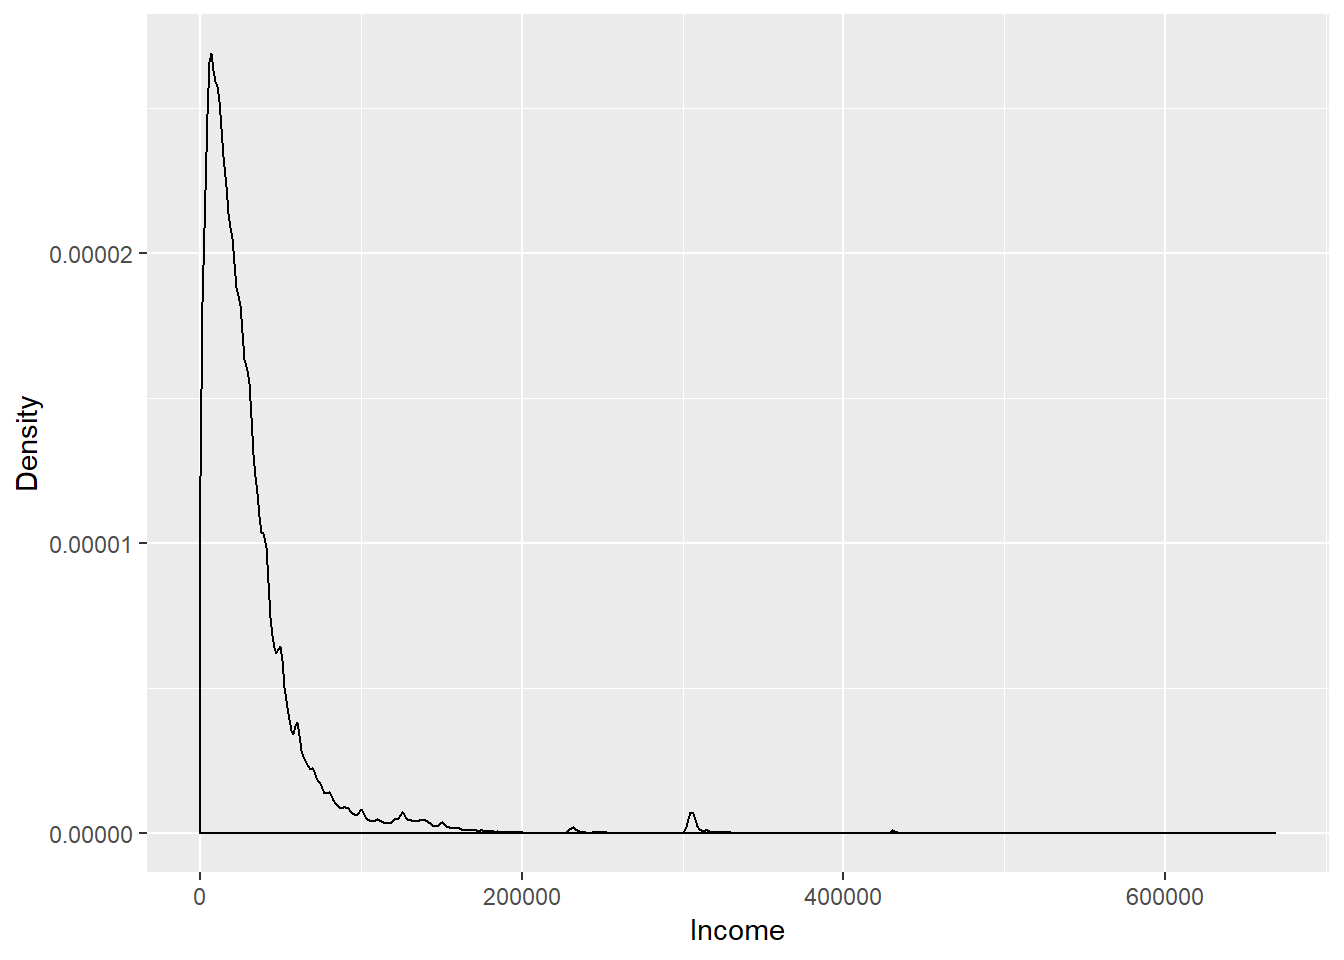
\includegraphics{05_Statistics_files/figure-latex/unnamed-chunk-3-1.pdf}

\begin{itemize}
\tightlist
\item
  The distribution has a long tail.
\item
  Let's plot the distribution in \emph{log} scale
\end{itemize}

\begin{Shaded}
\begin{Highlighting}[]
\CommentTok{# `log` option specifies which axis is represented in log scale.}
\KeywordTok{qplot}\NormalTok{(pop, }\DataTypeTok{geom =} \StringTok{"density"}\NormalTok{, }
      \DataTypeTok{xlab =} \StringTok{"Income"}\NormalTok{,}
      \DataTypeTok{ylab =} \StringTok{"Density"}\NormalTok{,}
      \DataTypeTok{log =} \StringTok{"x"}\NormalTok{)}
\end{Highlighting}
\end{Shaded}

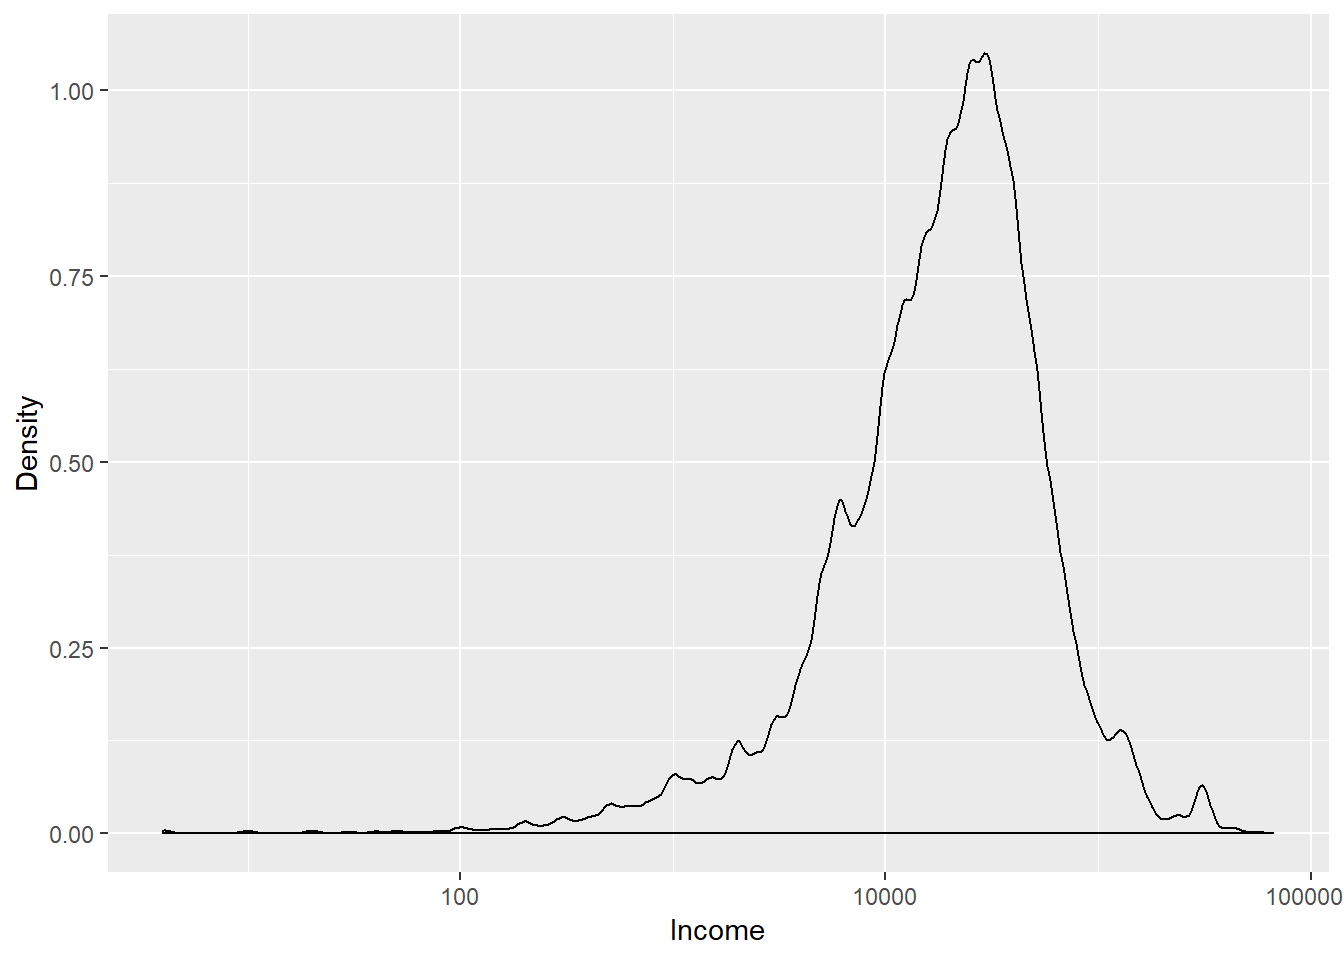
\includegraphics{05_Statistics_files/figure-latex/unnamed-chunk-4-1.pdf}

\begin{itemize}
\tightlist
\item
  Let's investigate how close the sample mean constucted from the random
  sample is to the true population mean.
\item
  Step 1: Draw random sample\emph{s} from this population and calculate
  \(\bar{Y}\) for each sample.

  \begin{itemize}
  \tightlist
  \item
    Set the sample size \(N\).
  \end{itemize}
\item
  Step 2: Repeat 2000 times. You now have 2000 sample means.
\end{itemize}

\begin{Shaded}
\begin{Highlighting}[]
\CommentTok{# Set the seed for the random number. This is needed to maintaine the reproducibility of the results.}
\KeywordTok{set.seed}\NormalTok{(}\DecValTok{123}\NormalTok{)}

\CommentTok{# draw random sample of 100 observations from the variable pop}
\NormalTok{test <-}\StringTok{ }\KeywordTok{sample}\NormalTok{(}\DataTypeTok{x =}\NormalTok{ pop, }\DataTypeTok{size =} \DecValTok{100}\NormalTok{)}

\CommentTok{# Use loop to repeat 2000 times. }
\NormalTok{Nsamples =}\StringTok{ }\DecValTok{2000}
\NormalTok{result1 <-}\StringTok{ }\KeywordTok{numeric}\NormalTok{(Nsamples)}

\ControlFlowTok{for}\NormalTok{ (i }\ControlFlowTok{in} \DecValTok{1}\OperatorTok{:}\NormalTok{Nsamples )\{}
  
\NormalTok{  test <-}\StringTok{ }\KeywordTok{sample}\NormalTok{(}\DataTypeTok{x =}\NormalTok{ pop, }\DataTypeTok{size =} \DecValTok{100}\NormalTok{)}
\NormalTok{  result1[i] <-}\StringTok{ }\KeywordTok{mean}\NormalTok{(test)}
  
\NormalTok{\}}

\CommentTok{# Simple approach}
\NormalTok{result1 <-}\StringTok{ }\KeywordTok{replicate}\NormalTok{(}\DataTypeTok{expr =} \KeywordTok{mean}\NormalTok{(}\KeywordTok{sample}\NormalTok{(}\DataTypeTok{x =}\NormalTok{ pop, }\DataTypeTok{size =} \DecValTok{10}\NormalTok{)), }\DataTypeTok{n =}\NormalTok{ Nsamples)}
\NormalTok{result2 <-}\StringTok{ }\KeywordTok{replicate}\NormalTok{(}\DataTypeTok{expr =} \KeywordTok{mean}\NormalTok{(}\KeywordTok{sample}\NormalTok{(}\DataTypeTok{x =}\NormalTok{ pop, }\DataTypeTok{size =} \DecValTok{100}\NormalTok{)), }\DataTypeTok{n =}\NormalTok{ Nsamples)}
\NormalTok{result3 <-}\StringTok{ }\KeywordTok{replicate}\NormalTok{(}\DataTypeTok{expr =} \KeywordTok{mean}\NormalTok{(}\KeywordTok{sample}\NormalTok{(}\DataTypeTok{x =}\NormalTok{ pop, }\DataTypeTok{size =} \DecValTok{500}\NormalTok{)), }\DataTypeTok{n =}\NormalTok{ Nsamples)}

\CommentTok{# Create dataframe}

\NormalTok{result_data <-}\StringTok{ }\KeywordTok{data.frame}\NormalTok{(  }\DataTypeTok{Ybar10 =}\NormalTok{ result1, }
                            \DataTypeTok{Ybar100 =}\NormalTok{ result2, }
                            \DataTypeTok{Ybar500 =}\NormalTok{ result3)}
\end{Highlighting}
\end{Shaded}

\begin{itemize}
\tightlist
\item
  Step 3: See the distribution of those 2000 sample means.
\end{itemize}

\begin{Shaded}
\begin{Highlighting}[]
\CommentTok{# Use reshape library}
\CommentTok{# install.packages("reshape")}
\KeywordTok{library}\NormalTok{(}\StringTok{"reshape"}\NormalTok{)}
\end{Highlighting}
\end{Shaded}

\begin{verbatim}
## Warning: パッケージ 'reshape' はバージョン 3.5.3 の R の下で造られました
\end{verbatim}

\begin{Shaded}
\begin{Highlighting}[]
\CommentTok{# Use "melt" to change the format of result_data}
\NormalTok{data_for_plot <-}\StringTok{ }\KeywordTok{melt}\NormalTok{(}\DataTypeTok{data =}\NormalTok{ result_data, }\DataTypeTok{variable.name =} \StringTok{"Variable"}\NormalTok{ )}
\end{Highlighting}
\end{Shaded}

\begin{verbatim}
## Using  as id variables
\end{verbatim}

\begin{Shaded}
\begin{Highlighting}[]
\CommentTok{# Use "ggplot2" to create the figure.}
\CommentTok{# The variable `fig` contains the information about the figure}
\NormalTok{fig <-}\StringTok{ }
\StringTok{  }\KeywordTok{ggplot}\NormalTok{(}\DataTypeTok{data =}\NormalTok{ data_for_plot) }\OperatorTok{+}
\StringTok{  }\KeywordTok{xlab}\NormalTok{(}\StringTok{"Sample mean"}\NormalTok{) }\OperatorTok{+}\StringTok{ }
\StringTok{  }\KeywordTok{geom_line}\NormalTok{(}\KeywordTok{aes}\NormalTok{(}\DataTypeTok{x =}\NormalTok{ value, }\DataTypeTok{colour =}\NormalTok{ variable ),   }\DataTypeTok{stat =} \StringTok{"density"}\NormalTok{ ) }\OperatorTok{+}\StringTok{ }
\StringTok{  }\KeywordTok{geom_vline}\NormalTok{(}\DataTypeTok{xintercept=}\NormalTok{pop_mean ,}\DataTypeTok{colour=}\StringTok{"black"}\NormalTok{)}

\CommentTok{# Display the figure }
\KeywordTok{plot}\NormalTok{(fig)}
\end{Highlighting}
\end{Shaded}

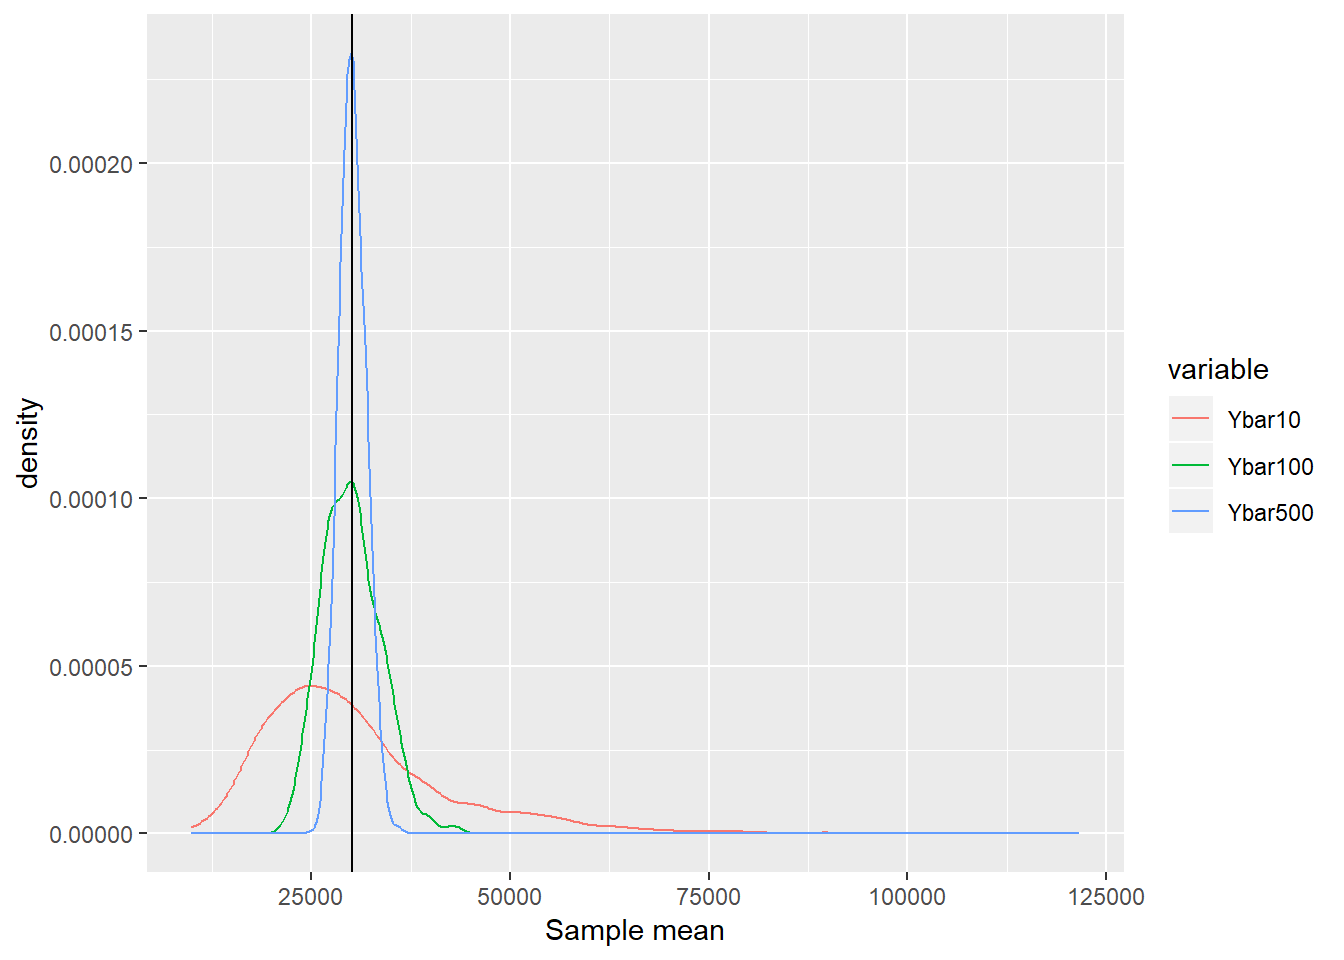
\includegraphics{05_Statistics_files/figure-latex/unnamed-chunk-6-1.pdf}

\begin{itemize}
\tightlist
\item
  Observation 1: Regardless of the sample size, the average of the
  sample means is close to the population mean. \textbf{Unbiasdeness}
\item
  Observation 2: As the sample size gets larger, the distribution is
  concentrated around the population mean. \textbf{Consistency (law of
  large numbers)}
\end{itemize}

\section{Hypothesis Testing}\label{hypothesis-testing}

\subsection{Central limit theorem}\label{central-limit-theorem}

\begin{itemize}
\item
  Cental limit theorem: Consider the i.i.d. sample of
  \(Y_1,\cdots, Y_N\) drawn from the random variable \(Y\) with mean
  \(\mu\) and variance \(\sigma^2\). The following \(Z\) converges in
  distribution to the normal distribution. \[
  Z = \frac{1}{\sqrt{N}} \sum_{i=1}^N \frac{Y_i - \mu}{\sigma } \overset{d}{\rightarrow}N(0,1)
  \] In other words, \[
  \lim_{N\rightarrow\infty}P\left(Z \leq z\right)=\Phi(z)
  \]
\item
  The central limit theorem implies that if \(N\) is large
  \textbf{enough}, we can \textbf{approximate} the distribution of
  \(\bar{Y}\) by the standard normal distribution with mean \(\mu\) and
  variance \(\sigma^2 / N\) \textbf{regardless of the underlying
  distribution of \(Y\).}
\item
  Let's examine this property through simulation!!
\item
  Use the same example as before. Remember that the underlying income
  distribution is clearly NOT normal.

  \begin{itemize}
  \tightlist
  \item
    Population mean \(\mu = 30165.4673315\) and standard deviation
    \(\sigma = 38306.1712336\). Use these numbers.
  \end{itemize}
\end{itemize}

\begin{Shaded}
\begin{Highlighting}[]
\CommentTok{# Set the seed for the random number}
\KeywordTok{set.seed}\NormalTok{(}\DecValTok{124}\NormalTok{)}

\CommentTok{# define function for simulation }
\NormalTok{f_simu_CLT =}\StringTok{ }\ControlFlowTok{function}\NormalTok{(Nsamples, samplesize, pop, pop_mean, pop_sd )\{}
  
\NormalTok{  output =}\StringTok{ }\KeywordTok{numeric}\NormalTok{(Nsamples)}
  \ControlFlowTok{for}\NormalTok{ (i }\ControlFlowTok{in} \DecValTok{1}\OperatorTok{:}\NormalTok{Nsamples )\{}
\NormalTok{    test <-}\StringTok{ }\KeywordTok{sample}\NormalTok{(}\DataTypeTok{x =}\NormalTok{ pop, }\DataTypeTok{size =}\NormalTok{ samplesize)}
\NormalTok{    output[i] <-}\StringTok{ }\NormalTok{( }\KeywordTok{mean}\NormalTok{(test) }\OperatorTok{-}\StringTok{ }\NormalTok{pop_mean ) }\OperatorTok{/}\StringTok{ }\NormalTok{(pop_sd }\OperatorTok{/}\StringTok{ }\KeywordTok{sqrt}\NormalTok{(samplesize))}
\NormalTok{  \}}
  
  \KeywordTok{return}\NormalTok{(output)}

\NormalTok{\}}

\CommentTok{# Comment: You can do better without using forloop. Let me know if you come with a good idea.}

\CommentTok{# Run simulation }
\NormalTok{Nsamples =}\StringTok{ }\DecValTok{2000}
\NormalTok{result_CLT1 <-}\StringTok{ }\KeywordTok{f_simu_CLT}\NormalTok{(Nsamples, }\DecValTok{10}\NormalTok{, pop, pop_mean, pop_sd )}
\NormalTok{result_CLT2 <-}\StringTok{ }\KeywordTok{f_simu_CLT}\NormalTok{(Nsamples, }\DecValTok{100}\NormalTok{, pop, pop_mean, pop_sd )}
\NormalTok{result_CLT3 <-}\StringTok{ }\KeywordTok{f_simu_CLT}\NormalTok{(Nsamples, }\DecValTok{1000}\NormalTok{, pop, pop_mean, pop_sd )}

\CommentTok{# Random draw from standard normal distribution as comparison}
\NormalTok{result_stdnorm =}\StringTok{ }\KeywordTok{rnorm}\NormalTok{(Nsamples)}

\CommentTok{# Create dataframe}
\NormalTok{result_CLT_data <-}\StringTok{ }\KeywordTok{data.frame}\NormalTok{(  }\DataTypeTok{Ybar_standardized_10 =}\NormalTok{ result_CLT1, }
                            \DataTypeTok{Ybar_standardized_100 =}\NormalTok{ result_CLT2, }
                            \DataTypeTok{Ybar_standardized_1000 =}\NormalTok{ result_CLT3, }
                            \DataTypeTok{Standard_Normal =}\NormalTok{ result_stdnorm)}

\CommentTok{# Note: If you wanna quicky plot the density, type `plot(density(result1))`. }
\end{Highlighting}
\end{Shaded}

\begin{itemize}
\tightlist
\item
  Now take a look at the distribution.
\end{itemize}

\begin{Shaded}
\begin{Highlighting}[]
\CommentTok{# Use "melt" to change the format of result_data}
\NormalTok{data_for_plot <-}\StringTok{ }\KeywordTok{melt}\NormalTok{(}\DataTypeTok{data =}\NormalTok{ result_CLT_data, }\DataTypeTok{variable.name =} \StringTok{"Variable"}\NormalTok{ )}
\end{Highlighting}
\end{Shaded}

\begin{verbatim}
## Using  as id variables
\end{verbatim}

\begin{Shaded}
\begin{Highlighting}[]
\CommentTok{# Use "ggplot2" to create the figure.}
\NormalTok{fig <-}\StringTok{ }
\StringTok{  }\KeywordTok{ggplot}\NormalTok{(}\DataTypeTok{data =}\NormalTok{ data_for_plot) }\OperatorTok{+}
\StringTok{  }\KeywordTok{xlab}\NormalTok{(}\StringTok{"Sample mean"}\NormalTok{) }\OperatorTok{+}\StringTok{ }
\StringTok{  }\KeywordTok{geom_line}\NormalTok{(}\KeywordTok{aes}\NormalTok{(}\DataTypeTok{x =}\NormalTok{ value, }\DataTypeTok{colour =}\NormalTok{ variable ),   }\DataTypeTok{stat =} \StringTok{"density"}\NormalTok{ ) }\OperatorTok{+}\StringTok{ }
\StringTok{  }\KeywordTok{geom_vline}\NormalTok{(}\DataTypeTok{xintercept=}\DecValTok{0}\NormalTok{ ,}\DataTypeTok{colour=}\StringTok{"black"}\NormalTok{)}

\KeywordTok{plot}\NormalTok{(fig)}
\end{Highlighting}
\end{Shaded}

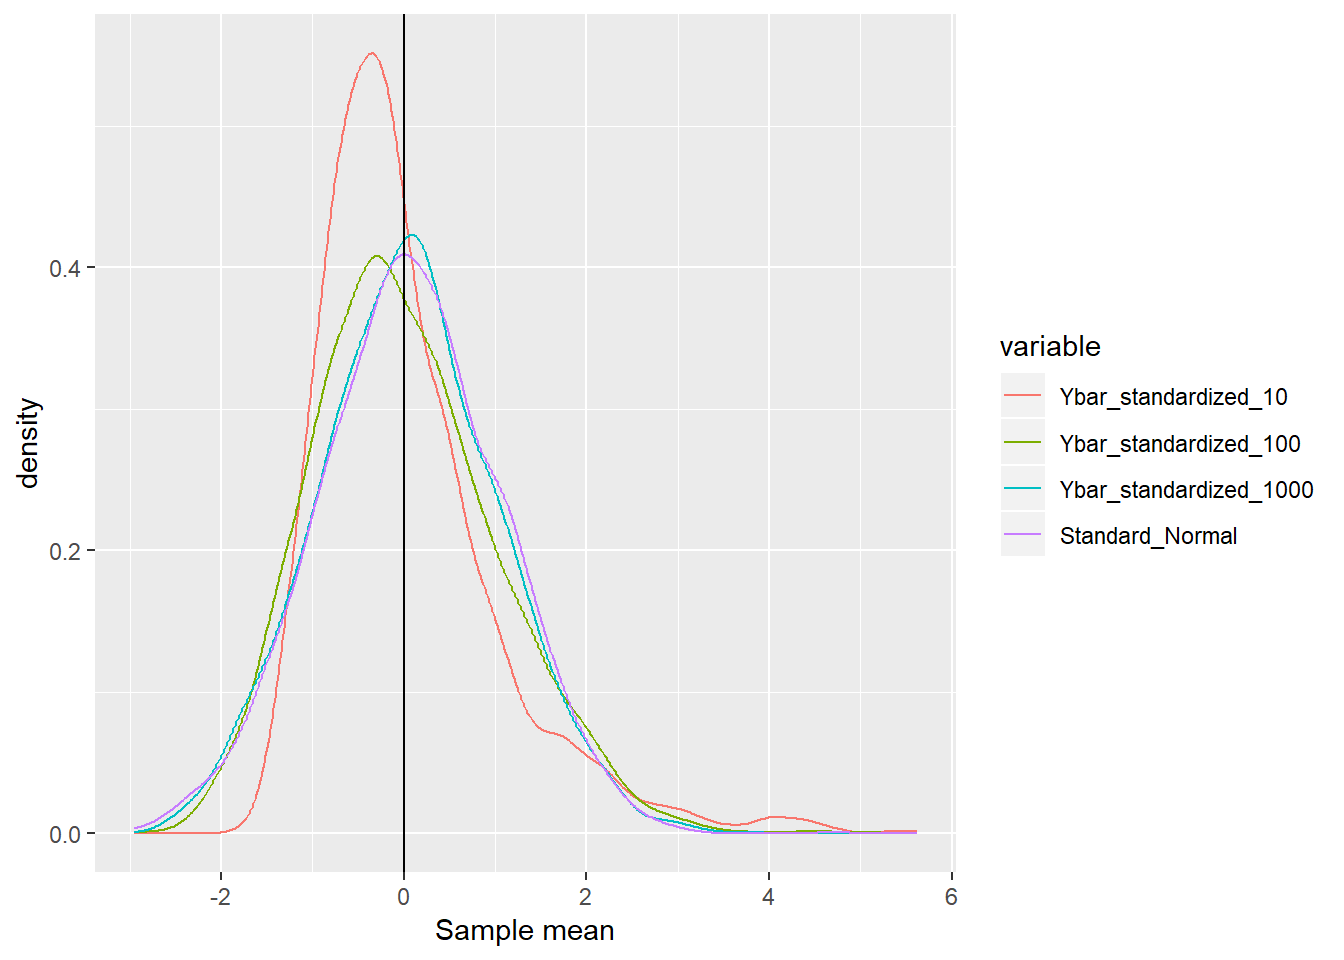
\includegraphics{05_Statistics_files/figure-latex/unnamed-chunk-8-1.pdf}

\begin{itemize}
\tightlist
\item
  As the sample size grows, the distribution of \(Z\) converges to the
  standard normal distribution.
\end{itemize}

\subsection{Hypothesis testing}\label{hypothesis-testing-1}

To be added.

\chapter{Linear Regression 1: Theory}\label{linear-regression-1-theory}

\section{Regression framework}\label{regression-framework}

\begin{itemize}
\tightlist
\item
  Let \(Y_i\) be the dependent variable and \(X_{ik}\) be k-th
  explanatory variable.

  \begin{itemize}
  \tightlist
  \item
    We have \(K\) explantory variables (along with constant term)
  \item
    \(i\) is an index for observations. \(i = 1,\cdots, N\).
  \item
    Data (sample): \(\{ Y_i , X_{i1}, \ldots, X_{iK} \}_{i=1}^N\)
  \end{itemize}
\item
  \textbf{Linear regression model} is defined as
  \[ Y_{i}=\beta_{0}+\beta_{1}X_{1i}+\cdots+\beta_{K}X_{Ki}+\epsilon_{i} \]

  \begin{itemize}
  \tightlist
  \item
    \(\epsilon_i\): error term (unobserved)
  \item
    \(\beta\): coefficients
  \end{itemize}
\item
  \textbf{Assumptions for Ordinaly Least Squares (OLS) estimation}

  \begin{enumerate}
  \def\labelenumi{\arabic{enumi}.}
  \tightlist
  \item
    Random sample: \(\{ Y_i , X_{i1}, \ldots, X_{iK} \}\) is i.i.d.
    drawn sample

    \begin{itemize}
    \tightlist
    \item
      i.i.d.: identically and independently distributed
    \end{itemize}
  \item
    \(\epsilon_i\) has zero conditional mean \[
      E[ \epsilon_i | X_{i1}, \ldots, X_{iK}] = 0
      \]
  \item
    Large outliers are unlikely: The random variable \(Y_i\) and
    \(X_{ik}\) have finite fourth moments.
  \item
    No perfect multicollinearity: There is no linear relationship betwen
    explanatory variables.
  \end{enumerate}
\item
  OLS estimators are the minimizers of the sum of squared residuals: \[
  \min_{\beta_0, \cdots, \beta_K} \frac{1}{N} \sum_{i=1}^N (Y_i - (\beta_0 + \beta_1 X_{i1} + \cdots + \beta_K X_{iK}))^2
  \]
\item
  Using matrix notation, we have the following analytical formula for
  the OLS estimator \[
  \hat{\beta} = (X'X)^{-1} X'Y
  \] where \[
  \underbrace{X}_{N\times (K+1)}=\left(\begin{array}{cccc}
  1 & X_{11} & \cdots & X_{1K}\\
  \vdots & \vdots &  & \vdots\\
  1 & X_{N1} & \cdots & X_{NK}
  \end{array}\right),\underbrace{Y}_{N\times 1}=\left(\begin{array}{c}
  Y_{1}\\
  \vdots\\
  Y_{N}
  \end{array}\right),\underbrace{\beta}_{(K+1)\times 1}=\left(\begin{array}{c}
  \beta_{0}\\
  \beta_{1}\\
  \vdots\\
  \beta_{K}
  \end{array}\right)            
  \]
\end{itemize}

\section{Theoretical Properties of OLS
estimator}\label{theoretical-properties-of-ols-estimator}

\begin{itemize}
\tightlist
\item
  We briefly review theoretical properties of OLS estimator.
\end{itemize}

\begin{enumerate}
\def\labelenumi{\arabic{enumi}.}
\tightlist
\item
  \textbf{Unbiasdness}: Conditional on the explantory variables \(X\),
  the expectation of the OLS estimator \(\hat{\beta}\) is equal to the
  true value \(\beta\). \[
  E[\hat{\beta} | X] = \beta
  \]
\item
  \textbf{Consistency}: As the sample size \(N\) goes to infinity, the
  OLS estimator \(\hat{\beta}\) converges to \(\beta\) in probability \[
  \hat{\beta}\overset{p}{\longrightarrow}\beta
  \]
\item
  \textbf{Asymptotic normality}: Will talk this
  \protect\hyperlink{Statistical-Inference}{later}
\end{enumerate}

\section{Interpretation and Specifications of Linear Regression
Model}\label{interpretation-and-specifications-of-linear-regression-model}

\begin{itemize}
\tightlist
\item
  Remember that \[ 
  Y_{i}=\beta_{0}+\beta_{1}X_{1i}+\cdots+\beta_{K}X_{Ki}+\epsilon_{i} 
  \]
\item
  The coefficient \(\beta_k\) captures the effect of \(X_k\) on \(Y\)
  \textbf{ceteris paribus (all things being equal)}
\item
  Equivalently, \[
  \frac{\partial Y}{\partial X_k} = \beta_k 
      \] if \(X_k\) is continuous random variable.
\item
  If we can estimate \(\beta_k\) without bias, we can obtain
  \textbf{causal effect} of \(X_k\) on \(Y\).

  \begin{itemize}
  \tightlist
  \item
    This is of course very difficult task. We will see this more later.
  \end{itemize}
\item
  We will see several specifications that are frequently used in
  empirical analysis. 1. Nonlinear term 1. log specification 2. dummy
  (categorical) variables 3. interaction terms
\end{itemize}

\subsection{Nonlinear term}\label{nonlinear-term}

\begin{itemize}
\tightlist
\item
  We can capture non-linear relationship between \(Y\) and \(X\) in a
  linearly additive form \[
  Y_i = \beta_0 + \beta_1 X_i + \beta_2 X_i^2 + \beta_3 X_i^3 + \epsilon_i
  \]
\item
  As long as the error term \(\epsilon_i\) appreas in a additively
  linear way, we can estimate the coefficients by OLS.

  \begin{itemize}
  \tightlist
  \item
    Multicollinarity could be an issue if we have many polynomials (see
    later).
  \item
    You can use other non-linear variables such as \(log(x)\) and
    \(\sqrt{x}\).
  \end{itemize}
\end{itemize}

\subsection{log specification}\label{log-specification}

\begin{itemize}
\tightlist
\item
  We often use \texttt{log} variables in both dependent and independent
  variables.
\item
  Using \texttt{log} changes the interpretation of the coefficient
  \(\beta\) in terms of scales.
\end{itemize}

\begin{longtable}[]{@{}lll@{}}
\toprule
Dependent variable & Explanatory variable &
interpretation\tabularnewline
\midrule
\endhead
\(Y\) & \(X\) & 1 unit increase in \(X\) causes \(\beta\) units change
in Y\tabularnewline
\(\log Y\) & \(X\) & 1 unit increase in \(X\) causes \(100 \beta \%\)
incchangerease in \(Y\)\tabularnewline
\(Y\) & \(\log X\) & \(1\%\) increase in \(X\) causes \(\beta / 100\)
unit change in \(Y\)\tabularnewline
\(\log Y\) & \(\log X\) & \(1\%\) increase in \(X\) causes \(\beta \%\)
change in \(Y\)\tabularnewline
\bottomrule
\end{longtable}

\subsection{Dummy variable}\label{dummy-variable}

\begin{itemize}
\tightlist
\item
  A dummy variable takes only 1 or 0. This is used to express
  qualititative information
\item
  Example: Dummy variable for race \[
  white_{i}=\begin{cases}
  1 & if\ white\\
  0 & otherwise
  \end{cases} 
     \]
\item
  The coefficient on a dummy variable captures the difference of the
  outcome \(Y\) between categories
\item
  Consider the linear regression \[
  Y_i = \beta_0 + \beta_1 white_i + \epsilon_i
  \] The coefficient \(\beta_1\) captures the difference of \(Y\)
  between white and non-white people.
\end{itemize}

\subsection{Interaction term}\label{interaction-term}

\begin{itemize}
\tightlist
\item
  You can add the interaction of two explanatory variables in the
  regression model.
\item
  For example: \[
  wage_i = \beta_0 + \beta_1 educ_i + \beta_2 white_i + \beta_3 educ_i \times white_i + \epsilon_i
  \] where \(wage_i\) is the earnings of person \(i\) and \(educ_i\) is
  the years of schooling for person \(i\).
\item
  The effect of \(educ_i\) is \[
  \frac{\partial wage_i}{\partial educ_i} = \beta_1 + \beta_3 white_i,
  \]
\item
  This allows for heterogenous effects of education across races.
\end{itemize}

\section{Measures of Fit}\label{measures-of-fit}

\begin{itemize}
\tightlist
\item
  We often use \(R^2\) as a measure of the model fit.
\item
  Denote \textbf{the fitted value} as \(\hat{y}_i\) \[
   \hat{y}_i = \hat{\beta}_0 + \hat{\beta}_1 X_{i1} + \cdots + \hat{\beta}_K X_{iK}
  \]

  \begin{itemize}
  \tightlist
  \item
    Also called prediction from the OLS regression.
  \end{itemize}
\item
  \(R^2\) is defined as \[
  R^2 = \frac{SSE}{TSS},
  \] where \[ 
   \  SSE = \sum_i (\hat{y}_i - \bar{y})^2, \ TSS = \sum_i (y_i - \bar{y})^2
  \]
\item
  \(R^2\) captures the fraction of the variation of \(Y\) explained by
  the regression model.
\item
  Adding variables always (weakly) increases \(R^2\).
\item
  In a regression model with multiple explanatory variables, we often
  use \textbf{adjusted} \(R^2\) that adjusts the number of explanatory
  variables \[
  \bar{R}^2 = 1 - \frac{N-1}{N-(K+1)} \frac{SSR}{TSS}
  \] where \[
  SSR = \sum_i (\hat{y}_i - y_i)^2 (= \sum_i \hat{u}_i^2 ),
  \]
\end{itemize}

\section{Statistical Inference}\label{statistical-inference}

\begin{itemize}
\tightlist
\item
  Notice that the OLS estimators are \textbf{random variables}. They
  depend on the data, which are random variables drawn from some
  population distribution.
\item
  We can conduct statistical inferences regarding those OLS estimators:
  1. Hypothesis testing 2. Constructing confidence interval
\item
  I first explain the sampling distribution of the OLS estimators.
\end{itemize}

\subsection{Distribution of the OLS estimators based on asymptotic
theory}\label{distribution-of-the-ols-estimators-based-on-asymptotic-theory}

\begin{itemize}
\tightlist
\item
  Deriving the exact (finite-sample) distribution of the OLS estimators
  is very hard.

  \begin{itemize}
  \tightlist
  \item
    The OLS estimators depend on the data \(Y_i, X_i\) in a complex way.
  \item
    We typically do not know the distribution of \(Y\) and \(X\).
  \end{itemize}
\item
  We rely on \textbf{asymptotic} argument. We approximate the sampling
  distribution of the OLS esimator based on the cental limit theorem.
\item
  Under the OLS assumption, the OLS estimator has \textbf{asymptotic
  normality} \[
  \sqrt{N}(\hat{\beta}-\beta)\overset{d}{\rightarrow}N\left(0,V \right)    
  \] where \[
  \underbrace{V}_{(K+1)\times(K+1)}
   = E[\mathbf{x}_{i}'\mathbf{x}_{i}]^{-1}E[\mathbf{x}_{i}'\mathbf{x}_{i}\epsilon_{i}^{2}]E[\mathbf{x}_{i}'\mathbf{x}_{i}]^{-1}
  \] and \[
  \underbrace{\mathbf{x}_{i}}_{(K+1)\times1}=\left(\begin{array}{c}
  1\\
  X_{i1}\\
  \vdots\\
  X_{iK}
  \end{array}\right)
  \]
\item
  We can \textbf{approximate} the distribution of \(\hat{\beta}\) by \[
  \hat{\beta} \sim N(\beta, V / N)
  \]
\item
  The above is joint distribution. Let \(V_{ij}\) be the \((i,j)\)
  element of the matrix \(V\).
\item
  The individual coefficient \(\beta_k\) follows \[
   \hat\beta_k \sim N(\beta_k, V_{kk} / N )
  \]
\end{itemize}

\subsubsection{Estimation of Asymptotic
Variance}\label{estimation-of-asymptotic-variance}

\begin{itemize}
\tightlist
\item
  \(V\) is an unknown object. Need to be estimated.
\item
  Consider the estimator \(\hat{V}\) for \(V\) using sample analogues \[
  \hat{V}=\left(\frac{1}{N}\sum_{i=1}^{N}\mathbf{x}_{i}'\mathbf{x}_{i}\right)^{-1}\left(\frac{1}{N}\sum_{i=1}^{N}\mathbf{x}_{i}'\mathbf{x}_{i}\hat{\epsilon}_{i}^{2}\right)\left(\frac{1}{N}\sum_{i=1}^{N}\mathbf{x}_{i}'\mathbf{x}_{i}\right)^{-1}
  \] where
  \(\hat{\epsilon}_i = y_i - (\hat{\beta}_0 + \cdots + \hat{\beta}_K X_{iK})\)
  is the residual.
\item
  Technically speaking, \(\hat{V}\) converges to \(V\) in probability.
  (Proof is out of the scope of this course)
\item
  We often use the (asymptotic) \textbf{standard error}
  \(SE(\hat{\beta_k}) = \sqrt{\hat{V}_{kk} / N }\).
\item
  The standard error is an estimator for the standard deviation of the
  OLS estimator \(\hat{\beta_k}\).
\end{itemize}

\subsection{Hypothesis testing}\label{hypothesis-testing-2}

\begin{itemize}
\item
  OLS estimator is the random variable.
\item
  You might want to test a particular hypothesis regarding those
  coefficients.

  \begin{itemize}
  \tightlist
  \item
    Does x really affects y?
  \item
    Is the production technology the constant returns to scale?
  \end{itemize}
\item
  Here I explain how to conduct hypothesis testing.
\item
  Step 1: Consider the null hypothesis \(H_{0}\) and the alternative
  hypothesis \(H_{1}\) \[
  H_{0}:\beta_{1}=k,H_{1}:\beta_{1}\neq k
  \] where \(k\) is the known number you set by yourself.
\item
  Step 2: Define \textbf{t-statistic} by \[
  t_{n}=\frac{\hat{\beta_1}-k}{SE(\hat{\beta_1})}
  \]
\item
  Step 3: We reject \(H_{0}\) is at \(\alpha\)-percent significance
  level if \[|t_{n}|>C_{\alpha/2} 
  \] where \(C_{\alpha/2}\) is the \(\alpha/2\) percentile of the
  standard normal distribution.

  \begin{itemize}
  \tightlist
  \item
    We say we \textbf{fail to reject} \(H_0\) if the above does not
    hold.
  \end{itemize}
\end{itemize}

\subsubsection{Caveats on Hypothesis
Testing}\label{caveats-on-hypothesis-testing}

\begin{itemize}
\tightlist
\item
  We often say \(\hat{\beta}\) is \textbf{statistically significant} at
  \(5\%\) level if \(|t_{n}|>1.96\) when we set \(k=0\).
\item
  Arguing the statistical significance alone is not enough for argument
  in empirical analysis.
\item
  Magnitude of the coefficient is also important.
\item
  Case 1: Small but statistically significant coefficient.

  \begin{itemize}
  \tightlist
  \item
    As the sample size \(N\) gets large, the \(SE\) decreases.
  \end{itemize}
\item
  Case 2: Large but statistically insignificant coefficient.

  \begin{itemize}
  \tightlist
  \item
    The variable might have an important (economically meaningful)
    effect.
  \item
    But you may not be able to estimate the effect precisely with the
    sample at your hand.
  \end{itemize}
\end{itemize}

\subsubsection{F test}\label{f-test}

\begin{itemize}
\tightlist
\item
  We often test a composite hypothesis that involves multiple parameters
  such as \[
   H_{0}:\beta_{1} + \beta_2 = 0,\ H_{1}:\beta_{1} + \beta_2 \neq 0
  \]
\item
  We use \textbf{F test} in such a case (to be added).
\end{itemize}

\subsection{Confidence interval}\label{confidence-interval}

\begin{itemize}
\tightlist
\item
  95\% confidence interval \[
  CI_{n}  =\left\{ k:|\frac{\hat{\beta}_{1}-k}{SE(\hat{\beta}_{1})}|\leq1.96\right\} 
  =\left[\hat{\beta}_{1}-1.96\times SE(\hat{\beta}_{1}),\hat{\beta_{1}}+1.96\times SE(\hat{\beta}_{1})\right]
  \]
\item
  Interpretation: If you draw many samples (dataset) and construct the
  95\% CI for each sample, 95\% of those CIs will include the true
  parameter.
\end{itemize}

\subsection{Homoskedasticity vs
Heteroskedasticity}\label{homoskedasticity-vs-heteroskedasticity}

\begin{itemize}
\tightlist
\item
  So far, we did not put any assumption on the variance of the error
  term \(\epsilon_i\).
\item
  The error term \(\epsilon_{i}\) has \textbf{heteroskedasticity} if
  \(Var(u_{i}|X_{i})\) depends on \(X_{i}\).
\item
  If not, we call \(\epsilon_{i}\) has \textbf{homoskedasticity}.
\item
  This has an important implication on the asymptotic variance.
\item
  Remember the asymptotic variance \[
  \underbrace{V}_{(K+1)\times(K+1)}
   = E[\mathbf{x}_{i}'\mathbf{x}_{i}]^{-1}E[\mathbf{x}_{i}'\mathbf{x}_{i}\epsilon_{i}^{2}]E[\mathbf{x}_{i}'\mathbf{x}_{i}]^{-1}
  \] Standard errors based on this is called \textbf{heteroskedasticity
  robust standard errors}/
\item
  If homoskedasticity holds, then \[
  V = E[\mathbf{x}_{i}'\mathbf{x}_{i}]^{-1}\sigma^{2}
  \] where \(\sigma^2 = V(\epsilon_i)\).
\item
  In many statistical packages (including R and Stata), the standard
  errors for the OLS estimators are calcualted under homoskedasticity
  assumption as a default.
\item
  However, if the error has heteroskedasticity, the standard error under
  homoskedasticity assumption will be \textbf{underestimated}.
\item
  In OLS, \textbf{we should always use heteroskedasticity robust
  standard error.}

  \begin{itemize}
  \tightlist
  \item
    We will see how to fix this in R.
  \end{itemize}
\end{itemize}

\chapter{Linear Regression 2: Implementation in
R}\label{linear-regression-2-implementation-in-r}

\section{Implementation in R}\label{implementation-in-r}

\subsection{Preliminary: packages}\label{preliminary-packages}

\begin{itemize}
\tightlist
\item
  We use the following packages:

  \begin{itemize}
  \tightlist
  \item
    \texttt{AER} :
  \item
    \texttt{dplyr} : data manipulation
  \item
    \texttt{stargazer} : output of regression results
  \end{itemize}
\end{itemize}

\begin{Shaded}
\begin{Highlighting}[]
\CommentTok{# Install package if you have not done so }
\CommentTok{# install.packages("AER")}
\CommentTok{# install.packages("dplyr")}
\CommentTok{# install.packages("stargazer")}
\CommentTok{# install.packages("lmtest")}

\CommentTok{# load packages}
\KeywordTok{library}\NormalTok{(}\StringTok{"AER"}\NormalTok{)}
\end{Highlighting}
\end{Shaded}

\begin{verbatim}
##  要求されたパッケージ car をロード中です
\end{verbatim}

\begin{verbatim}
##  要求されたパッケージ carData をロード中です
\end{verbatim}

\begin{verbatim}
##  要求されたパッケージ lmtest をロード中です
\end{verbatim}

\begin{verbatim}
##  要求されたパッケージ zoo をロード中です
\end{verbatim}

\begin{verbatim}
## 
##  次のパッケージを付け加えます: 'zoo'
\end{verbatim}

\begin{verbatim}
##  以下のオブジェクトは 'package:base' からマスクされています: 
## 
##      as.Date, as.Date.numeric
\end{verbatim}

\begin{verbatim}
##  要求されたパッケージ sandwich をロード中です
\end{verbatim}

\begin{verbatim}
##  要求されたパッケージ survival をロード中です
\end{verbatim}

\begin{Shaded}
\begin{Highlighting}[]
\KeywordTok{library}\NormalTok{(}\StringTok{"dplyr"}\NormalTok{)}
\end{Highlighting}
\end{Shaded}

\begin{verbatim}
## 
##  次のパッケージを付け加えます: 'dplyr'
\end{verbatim}

\begin{verbatim}
##  以下のオブジェクトは 'package:car' からマスクされています: 
## 
##      recode
\end{verbatim}

\begin{verbatim}
##  以下のオブジェクトは 'package:stats' からマスクされています: 
## 
##      filter, lag
\end{verbatim}

\begin{verbatim}
##  以下のオブジェクトは 'package:base' からマスクされています: 
## 
##      intersect, setdiff, setequal, union
\end{verbatim}

\begin{Shaded}
\begin{Highlighting}[]
\KeywordTok{library}\NormalTok{(}\StringTok{"stargazer"}\NormalTok{)}
\end{Highlighting}
\end{Shaded}

\begin{verbatim}
## 
## Please cite as:
\end{verbatim}

\begin{verbatim}
##  Hlavac, Marek (2018). stargazer: Well-Formatted Regression and Summary Statistics Tables.
\end{verbatim}

\begin{verbatim}
##  R package version 5.2.2. https://CRAN.R-project.org/package=stargazer
\end{verbatim}

\begin{Shaded}
\begin{Highlighting}[]
\KeywordTok{library}\NormalTok{(}\StringTok{"lmtest"}\NormalTok{)}
\end{Highlighting}
\end{Shaded}

\subsection{Empirical setting: Data from California
School}\label{empirical-setting-data-from-california-school}

\begin{itemize}
\tightlist
\item
  Question: How does the student-teacher ratio affects test scores?
\item
  We use data from California school, which is included in \texttt{AER}
  package.

  \begin{itemize}
  \tightlist
  \item
    See here for the details:
    \url{https://www.rdocumentation.org/packages/AER/versions/1.2-6/topics/CASchools}
  \end{itemize}
\end{itemize}

\begin{Shaded}
\begin{Highlighting}[]
\CommentTok{# load the the data set in the workspace}
\KeywordTok{data}\NormalTok{(CASchools)}
\end{Highlighting}
\end{Shaded}

\begin{itemize}
\tightlist
\item
  Use \texttt{class()} function to see \texttt{CASchools} is
  \texttt{data.frame} object.
\end{itemize}

\begin{Shaded}
\begin{Highlighting}[]
\KeywordTok{class}\NormalTok{(CASchools)}
\end{Highlighting}
\end{Shaded}

\begin{verbatim}
## [1] "data.frame"
\end{verbatim}

\begin{itemize}
\tightlist
\item
  We take 2 steps for the analysis.

  \begin{itemize}
  \tightlist
  \item
    Step 1: Look at data (descriptive analysis)
  \item
    Step 2: Run regression
  \end{itemize}
\end{itemize}

\subsection{Step 1: Descriptive
analysis}\label{step-1-descriptive-analysis}

\begin{itemize}
\tightlist
\item
  It is always important to grasp your data before running regression.
\item
  \texttt{head()} function give you a first overview of the data.
\end{itemize}

\begin{Shaded}
\begin{Highlighting}[]
\KeywordTok{head}\NormalTok{(CASchools)}
\end{Highlighting}
\end{Shaded}

\begin{verbatim}
##   district                          school  county grades students
## 1    75119              Sunol Glen Unified Alameda  KK-08      195
## 2    61499            Manzanita Elementary   Butte  KK-08      240
## 3    61549     Thermalito Union Elementary   Butte  KK-08     1550
## 4    61457 Golden Feather Union Elementary   Butte  KK-08      243
## 5    61523        Palermo Union Elementary   Butte  KK-08     1335
## 6    62042         Burrel Union Elementary  Fresno  KK-08      137
##   teachers calworks   lunch computer expenditure    income   english  read
## 1    10.90   0.5102  2.0408       67    6384.911 22.690001  0.000000 691.6
## 2    11.15  15.4167 47.9167      101    5099.381  9.824000  4.583333 660.5
## 3    82.90  55.0323 76.3226      169    5501.955  8.978000 30.000002 636.3
## 4    14.00  36.4754 77.0492       85    7101.831  8.978000  0.000000 651.9
## 5    71.50  33.1086 78.4270      171    5235.988  9.080333 13.857677 641.8
## 6     6.40  12.3188 86.9565       25    5580.147 10.415000 12.408759 605.7
##    math
## 1 690.0
## 2 661.9
## 3 650.9
## 4 643.5
## 5 639.9
## 6 605.4
\end{verbatim}

\begin{itemize}
\tightlist
\item
  Alternatively, you can use \texttt{browse()} to see the entire dataset
  in browser window.
\end{itemize}

\subsubsection{Create variables}\label{create-variables}

\begin{itemize}
\tightlist
\item
  Create several variables that are needed for the analysis.
\item
  We use \texttt{dplyr} for this purpose.
\end{itemize}

\begin{Shaded}
\begin{Highlighting}[]
\NormalTok{CASchools }\OperatorTok\StringTok{ }
\StringTok{  }\KeywordTok{mutate}\NormalTok{( }\DataTypeTok{STR =}\NormalTok{ students }\OperatorTok{/}\StringTok{ }\NormalTok{teachers ) }\OperatorTok\StringTok{ }
\StringTok{  }\KeywordTok{mutate}\NormalTok{( }\DataTypeTok{score =}\NormalTok{ (read }\OperatorTok{+}\StringTok{ }\NormalTok{math) }\OperatorTok{/}\StringTok{ }\DecValTok{2}\NormalTok{ ) ->}\StringTok{ }\NormalTok{CASchools }
\end{Highlighting}
\end{Shaded}

\subsubsection{Descriptive statistics}\label{descriptive-statistics}

\begin{itemize}
\tightlist
\item
  There are several ways to show descriptive statistics
\item
  The standard one is to use \texttt{summary()} function
\end{itemize}

\begin{Shaded}
\begin{Highlighting}[]
\KeywordTok{summary}\NormalTok{(CASchools)}
\end{Highlighting}
\end{Shaded}

\begin{verbatim}
##    district            school                  county      grades   
##  Length:420         Length:420         Sonoma     : 29   KK-06: 61  
##  Class :character   Class :character   Kern       : 27   KK-08:359  
##  Mode  :character   Mode  :character   Los Angeles: 27              
##                                        Tulare     : 24              
##                                        San Diego  : 21              
##                                        Santa Clara: 20              
##                                        (Other)    :272              
##     students          teachers          calworks          lunch       
##  Min.   :   81.0   Min.   :   4.85   Min.   : 0.000   Min.   :  0.00  
##  1st Qu.:  379.0   1st Qu.:  19.66   1st Qu.: 4.395   1st Qu.: 23.28  
##  Median :  950.5   Median :  48.56   Median :10.520   Median : 41.75  
##  Mean   : 2628.8   Mean   : 129.07   Mean   :13.246   Mean   : 44.71  
##  3rd Qu.: 3008.0   3rd Qu.: 146.35   3rd Qu.:18.981   3rd Qu.: 66.86  
##  Max.   :27176.0   Max.   :1429.00   Max.   :78.994   Max.   :100.00  
##                                                                       
##     computer       expenditure       income          english      
##  Min.   :   0.0   Min.   :3926   Min.   : 5.335   Min.   : 0.000  
##  1st Qu.:  46.0   1st Qu.:4906   1st Qu.:10.639   1st Qu.: 1.941  
##  Median : 117.5   Median :5215   Median :13.728   Median : 8.778  
##  Mean   : 303.4   Mean   :5312   Mean   :15.317   Mean   :15.768  
##  3rd Qu.: 375.2   3rd Qu.:5601   3rd Qu.:17.629   3rd Qu.:22.970  
##  Max.   :3324.0   Max.   :7712   Max.   :55.328   Max.   :85.540  
##                                                                   
##       read            math            STR            score      
##  Min.   :604.5   Min.   :605.4   Min.   :14.00   Min.   :605.5  
##  1st Qu.:640.4   1st Qu.:639.4   1st Qu.:18.58   1st Qu.:640.0  
##  Median :655.8   Median :652.5   Median :19.72   Median :654.5  
##  Mean   :655.0   Mean   :653.3   Mean   :19.64   Mean   :654.2  
##  3rd Qu.:668.7   3rd Qu.:665.9   3rd Qu.:20.87   3rd Qu.:666.7  
##  Max.   :704.0   Max.   :709.5   Max.   :25.80   Max.   :706.8  
## 
\end{verbatim}

\begin{itemize}
\tightlist
\item
  This returns the desriptive statistics for all the variables in
  dataframe.
\item
  You can combine this with \texttt{dplyr::select}
\end{itemize}

\begin{Shaded}
\begin{Highlighting}[]
\NormalTok{CASchools }\OperatorTok\StringTok{ }
\StringTok{  }\KeywordTok{select}\NormalTok{(STR, score) }\OperatorTok
\StringTok{  }\KeywordTok{summary}\NormalTok{()}
\end{Highlighting}
\end{Shaded}

\begin{verbatim}
##       STR            score      
##  Min.   :14.00   Min.   :605.5  
##  1st Qu.:18.58   1st Qu.:640.0  
##  Median :19.72   Median :654.5  
##  Mean   :19.64   Mean   :654.2  
##  3rd Qu.:20.87   3rd Qu.:666.7  
##  Max.   :25.80   Max.   :706.8
\end{verbatim}

\begin{itemize}
\tightlist
\item
  You can do a bit lengthly thing manually like this.
\end{itemize}

\begin{Shaded}
\begin{Highlighting}[]
\CommentTok{# compute sample averages of STR and score}
\NormalTok{avg_STR <-}\StringTok{ }\KeywordTok{mean}\NormalTok{(CASchools}\OperatorTok{$}\NormalTok{STR) }
\NormalTok{avg_score <-}\StringTok{ }\KeywordTok{mean}\NormalTok{(CASchools}\OperatorTok{$}\NormalTok{score)}

\CommentTok{# compute sample standard deviations of STR and score}
\NormalTok{sd_STR <-}\StringTok{ }\KeywordTok{sd}\NormalTok{(CASchools}\OperatorTok{$}\NormalTok{STR) }
\NormalTok{sd_score <-}\StringTok{ }\KeywordTok{sd}\NormalTok{(CASchools}\OperatorTok{$}\NormalTok{score)}

\CommentTok{# set up a vector of percentiles and compute the quantiles }
\NormalTok{quantiles <-}\StringTok{ }\KeywordTok{c}\NormalTok{(}\FloatTok{0.10}\NormalTok{, }\FloatTok{0.25}\NormalTok{, }\FloatTok{0.4}\NormalTok{, }\FloatTok{0.5}\NormalTok{, }\FloatTok{0.6}\NormalTok{, }\FloatTok{0.75}\NormalTok{, }\FloatTok{0.9}\NormalTok{)}
\NormalTok{quant_STR <-}\StringTok{ }\KeywordTok{quantile}\NormalTok{(CASchools}\OperatorTok{$}\NormalTok{STR, quantiles)}
\NormalTok{quant_score <-}\StringTok{ }\KeywordTok{quantile}\NormalTok{(CASchools}\OperatorTok{$}\NormalTok{score, quantiles)}

\CommentTok{# gather everything in a data.frame }
\NormalTok{DistributionSummary <-}\StringTok{ }\KeywordTok{data.frame}\NormalTok{(}\DataTypeTok{Average =} \KeywordTok{c}\NormalTok{(avg_STR, avg_score), }
                                  \DataTypeTok{StandardDeviation =} \KeywordTok{c}\NormalTok{(sd_STR, sd_score), }
                                  \DataTypeTok{quantile =} \KeywordTok{rbind}\NormalTok{(quant_STR, quant_score))}

\CommentTok{# print the summary to the console}
\NormalTok{DistributionSummary}
\end{Highlighting}
\end{Shaded}

\begin{verbatim}
##               Average StandardDeviation quantile.10. quantile.25.
## quant_STR    19.64043          1.891812      17.3486     18.58236
## quant_score 654.15655         19.053347     630.3950    640.05000
##             quantile.40. quantile.50. quantile.60. quantile.75.
## quant_STR       19.26618     19.72321      20.0783     20.87181
## quant_score    649.06999    654.45000     659.4000    666.66249
##             quantile.90.
## quant_STR       21.86741
## quant_score    678.85999
\end{verbatim}

\begin{itemize}
\tightlist
\item
  My personal favorite is to use \texttt{stargazer} function.
\end{itemize}

\begin{Shaded}
\begin{Highlighting}[]
\KeywordTok{stargazer}\NormalTok{(CASchools, }\DataTypeTok{type =} \StringTok{"text"}\NormalTok{)}
\end{Highlighting}
\end{Shaded}

\begin{verbatim}
## 
## ===========================================================================
## Statistic    N    Mean    St. Dev.     Min    Pctl(25)  Pctl(75)     Max   
## ---------------------------------------------------------------------------
## students    420 2,628.793 3,913.105    81        379      3,008    27,176  
## teachers    420  129.067   187.913    4.850    19.662    146.350  1,429.000
## calworks    420  13.246    11.455     0.000     4.395    18.981    78.994  
## lunch       420  44.705    27.123     0.000    23.282    66.865    100.000 
## computer    420  303.383   441.341      0        46       375.2     3,324  
## expenditure 420 5,312.408  633.937  3,926.070 4,906.180 5,601.401 7,711.507
## income      420  15.317     7.226     5.335    10.639    17.629    55.328  
## english     420  15.768    18.286       0        1.9      23.0       86    
## read        420  654.970   20.108    604.500   640.400   668.725   704.000 
## math        420  653.343   18.754      605      639.4     665.8      710   
## STR         420  19.640     1.892    14.000    18.582    20.872    25.800  
## score       420  654.157   19.053    605.550   640.050   666.662   706.750 
## ---------------------------------------------------------------------------
\end{verbatim}

\begin{itemize}
\tightlist
\item
  You can choose summary statistics you want to report.
\end{itemize}

\begin{Shaded}
\begin{Highlighting}[]
\NormalTok{CASchools }\OperatorTok\StringTok{ }
\StringTok{  }\KeywordTok{stargazer}\NormalTok{( }\DataTypeTok{type =} \StringTok{"text"}\NormalTok{, }\DataTypeTok{summary.stat =} \KeywordTok{c}\NormalTok{(}\StringTok{"n"}\NormalTok{, }\StringTok{"p75"}\NormalTok{, }\StringTok{"sd"}\NormalTok{) ) }
\end{Highlighting}
\end{Shaded}

\begin{verbatim}
## 
## ===================================
## Statistic    N  Pctl(75)  St. Dev. 
## -----------------------------------
## students    420   3,008   3,913.105
## teachers    420  146.350   187.913 
## calworks    420  18.981    11.455  
## lunch       420  66.865    27.123  
## computer    420   375.2    441.341 
## expenditure 420 5,601.401  633.937 
## income      420  17.629     7.226  
## english     420   23.0     18.286  
## read        420  668.725   20.108  
## math        420   665.8    18.754  
## STR         420  20.872     1.892  
## score       420  666.662   19.053  
## -----------------------------------
\end{verbatim}

\begin{itemize}
\tightlist
\item
  See
  \url{https://www.jakeruss.com/cheatsheets/stargazer/\#the-default-summary-statistics-table}
  for the details.
\item
  We will use \texttt{stargazer} to report regression results.
\end{itemize}

\subsubsection{Scatter plot}\label{scatter-plot}

\begin{itemize}
\tightlist
\item
  Let's see how test score and student-teacher-ratio is correlated.
\end{itemize}

\begin{Shaded}
\begin{Highlighting}[]
\KeywordTok{plot}\NormalTok{(score }\OperatorTok{~}\StringTok{ }\NormalTok{STR, }
     \DataTypeTok{data =}\NormalTok{ CASchools,}
     \DataTypeTok{main =} \StringTok{"Scatterplot of TestScore and STR"}\NormalTok{, }
     \DataTypeTok{xlab =} \StringTok{"STR (X)"}\NormalTok{,}
     \DataTypeTok{ylab =} \StringTok{"Test Score (Y)"}\NormalTok{)}
\end{Highlighting}
\end{Shaded}

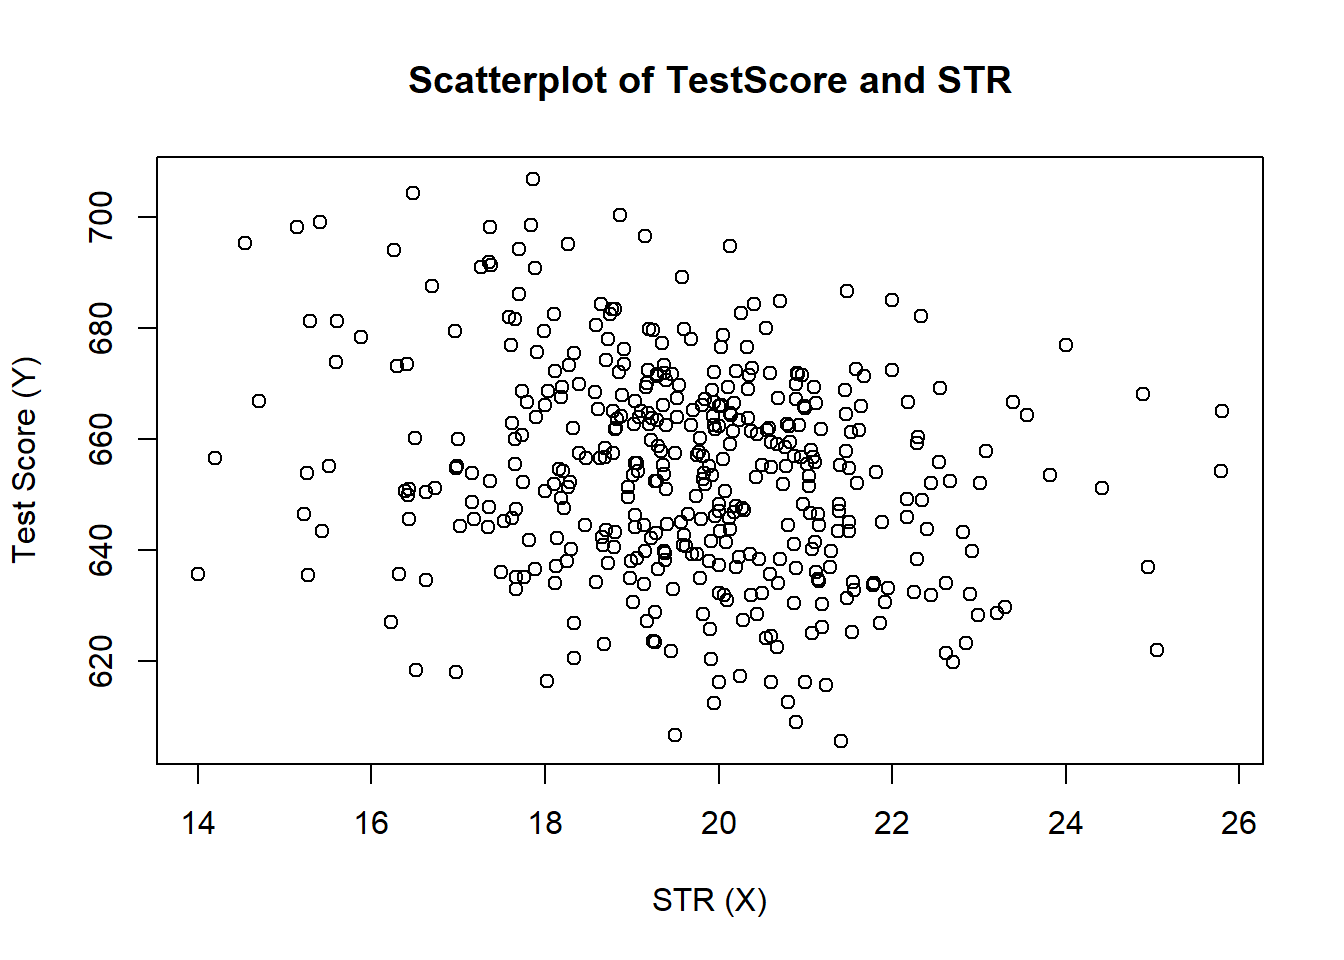
\includegraphics{07_Regression2_files/figure-latex/unnamed-chunk-11-1.pdf}

\begin{itemize}
\tightlist
\item
  Use \texttt{cor()} to compute the correlation between two numeric
  vectors.
\end{itemize}

\begin{Shaded}
\begin{Highlighting}[]
\KeywordTok{cor}\NormalTok{(CASchools}\OperatorTok{$}\NormalTok{STR, CASchools}\OperatorTok{$}\NormalTok{score)}
\end{Highlighting}
\end{Shaded}

\begin{verbatim}
## [1] -0.2263627
\end{verbatim}

\subsection{Step 2: Run regression}\label{step-2-run-regression}

\subsubsection{Simple linear regression}\label{simple-linear-regression}

\begin{itemize}
\tightlist
\item
  We use \texttt{lm()} function to run linear regression
\item
  First, consider the simple linear regression \[
  score_i = \beta_0 + \beta_1 size_i + \epsilon_i
  \] where \(size_i\) is the class size (student-teacher-ratio).

  \begin{itemize}
  \tightlist
  \item
    From now on we call student-teacher-ratio (STR) class size.
  \end{itemize}
\item
  To run this regression, we use \texttt{lm}
\end{itemize}

\begin{Shaded}
\begin{Highlighting}[]
\CommentTok{# First, we rename the variable `STR`}
\NormalTok{CASchools }\OperatorTok\StringTok{ }
\StringTok{  }\NormalTok{dplyr}\OperatorTok{::}\KeywordTok{rename}\NormalTok{( }\DataTypeTok{size =}\NormalTok{ STR) ->}\StringTok{ }\NormalTok{CASchools}

\CommentTok{# Run regression and save results in the varaiable `model1_summary`}
\NormalTok{model1_summary <-}\StringTok{ }\KeywordTok{lm}\NormalTok{( score }\OperatorTok{~}\StringTok{ }\NormalTok{size, }\DataTypeTok{data =}\NormalTok{ CASchools)}

\CommentTok{# See the results}
\KeywordTok{summary}\NormalTok{(model1_summary)}
\end{Highlighting}
\end{Shaded}

\begin{verbatim}
## 
## Call:
## lm(formula = score ~ size, data = CASchools)
## 
## Residuals:
##     Min      1Q  Median      3Q     Max 
## -47.727 -14.251   0.483  12.822  48.540 
## 
## Coefficients:
##             Estimate Std. Error t value             Pr(>|t|)    
## (Intercept) 698.9329     9.4675  73.825 < 0.0000000000000002 ***
## size         -2.2798     0.4798  -4.751           0.00000278 ***
## ---
## Signif. codes:  0 '***' 0.001 '**' 0.01 '*' 0.05 '.' 0.1 ' ' 1
## 
## Residual standard error: 18.58 on 418 degrees of freedom
## Multiple R-squared:  0.05124,    Adjusted R-squared:  0.04897 
## F-statistic: 22.58 on 1 and 418 DF,  p-value: 0.000002783
\end{verbatim}

\begin{itemize}
\tightlist
\item
  Interpretations

  \begin{itemize}
  \tightlist
  \item
    An increase of one student per teacher leads to 2.2 point decrease
    in test scores.
  \item
    p value is very small. The effect of the class size on test score is
    significant. Note: Be careful. These standard errors are NOT
    heteroskedasiticity robust. We will come back to this point soon.
  \item
    \(R^2 = 0.051\), implying that 5.1\% of the variance of the
    dependent variable is explained by the model.
  \end{itemize}
\item
  You can add more variable in the regression (will see this soon)
\end{itemize}

\subsubsection{Correction of Robust standard
error}\label{correction-of-robust-standard-error}

\begin{itemize}
\tightlist
\item
  We use \texttt{vcovHC()} function, a partof the package
  \texttt{sandwich}, to obtain the robust standard errors.

  \begin{itemize}
  \tightlist
  \item
    The package \texttt{sandwich} is automatically loaded if you load
    \texttt{AER} package.
  \end{itemize}
\end{itemize}

\begin{Shaded}
\begin{Highlighting}[]
\CommentTok{# compute heteroskedasticity-robust standard errors}
\NormalTok{vcov <-}\StringTok{ }\KeywordTok{vcovHC}\NormalTok{(model1_summary, }\DataTypeTok{type =} \StringTok{"HC1"}\NormalTok{)}

\CommentTok{# get standard error: the square root of the diagonal element in vcov}
\NormalTok{robust_se <-}\StringTok{ }\KeywordTok{sqrt}\NormalTok{(}\KeywordTok{diag}\NormalTok{(vcov))}
\NormalTok{robust_se}
\end{Highlighting}
\end{Shaded}

\begin{verbatim}
## (Intercept)        size 
##  10.3643617   0.5194893
\end{verbatim}

\begin{itemize}
\tightlist
\item
  Notice that robust standard errors are larger than the one we obtained
  from \texttt{lm}!
\item
  How to combine the robust standard errors with the original summary?
  Use \texttt{coeftest()} from the package \texttt{lmtest}
\end{itemize}

\begin{Shaded}
\begin{Highlighting}[]
\CommentTok{# load `lmtest`}
\KeywordTok{library}\NormalTok{(lmtest)}

\CommentTok{# Combine robust standard errors}
\KeywordTok{coeftest}\NormalTok{(model1_summary, }\DataTypeTok{vcov. =}\NormalTok{ vcov)}
\end{Highlighting}
\end{Shaded}

\begin{verbatim}
## 
## t test of coefficients:
## 
##              Estimate Std. Error t value              Pr(>|t|)    
## (Intercept) 698.93295   10.36436 67.4362 < 0.00000000000000022 ***
## size         -2.27981    0.51949 -4.3886            0.00001447 ***
## ---
## Signif. codes:  0 '***' 0.001 '**' 0.01 '*' 0.05 '.' 0.1 ' ' 1
\end{verbatim}

\subsubsection{Report by Stargazer}\label{report-by-stargazer}

\begin{itemize}
\tightlist
\item
  \texttt{stargazer} is useful to show the regression result.
\end{itemize}

\begin{Shaded}
\begin{Highlighting}[]
\CommentTok{# load}
\KeywordTok{library}\NormalTok{(stargazer)}

\CommentTok{# Create output by stargazer}
\NormalTok{stargazer}\OperatorTok{::}\KeywordTok{stargazer}\NormalTok{(model1_summary, }\DataTypeTok{type =}\StringTok{"text"}\NormalTok{)}
\end{Highlighting}
\end{Shaded}

\begin{verbatim}
## 
## ===============================================
##                         Dependent variable:    
##                     ---------------------------
##                                score           
## -----------------------------------------------
## size                         -2.280***         
##                               (0.480)          
##                                                
## Constant                    698.933***         
##                               (9.467)          
##                                                
## -----------------------------------------------
## Observations                    420            
## R2                             0.051           
## Adjusted R2                    0.049           
## Residual Std. Error      18.581 (df = 418)     
## F Statistic           22.575*** (df = 1; 418)  
## ===============================================
## Note:               *p<0.1; **p<0.05; ***p<0.01
\end{verbatim}

\begin{itemize}
\tightlist
\item
  Use robust standard errors in stargazer output
\end{itemize}

\begin{Shaded}
\begin{Highlighting}[]
\CommentTok{# Prepare robust standard errors in list}
\NormalTok{rob_se <-}\StringTok{ }\KeywordTok{list}\NormalTok{( }\KeywordTok{sqrt}\NormalTok{(}\KeywordTok{diag}\NormalTok{(}\KeywordTok{vcovHC}\NormalTok{(model1_summary, }\DataTypeTok{type =} \StringTok{"HC1"}\NormalTok{) ) ) ) }

\CommentTok{# generate regression table. }

\KeywordTok{stargazer}\NormalTok{( model1_summary, }
           \DataTypeTok{se =}\NormalTok{ rob_se, }
           \DataTypeTok{type =} \StringTok{"text"}\NormalTok{)}
\end{Highlighting}
\end{Shaded}

\begin{verbatim}
## 
## ===============================================
##                         Dependent variable:    
##                     ---------------------------
##                                score           
## -----------------------------------------------
## size                         -2.280***         
##                               (0.519)          
##                                                
## Constant                    698.933***         
##                              (10.364)          
##                                                
## -----------------------------------------------
## Observations                    420            
## R2                             0.051           
## Adjusted R2                    0.049           
## Residual Std. Error      18.581 (df = 418)     
## F Statistic           22.575*** (df = 1; 418)  
## ===============================================
## Note:               *p<0.1; **p<0.05; ***p<0.01
\end{verbatim}

\subsubsection{Full results}\label{full-results}

Taken from
\url{https://www.econometrics-with-r.org/7-6-analysis-of-the-test-score-data-set.html}

\begin{Shaded}
\begin{Highlighting}[]
\CommentTok{# load the stargazer library}

\CommentTok{# estimate different model specifications}
\NormalTok{spec1 <-}\StringTok{ }\KeywordTok{lm}\NormalTok{(score }\OperatorTok{~}\StringTok{ }\NormalTok{size, }\DataTypeTok{data =}\NormalTok{ CASchools)}
\NormalTok{spec2 <-}\StringTok{ }\KeywordTok{lm}\NormalTok{(score }\OperatorTok{~}\StringTok{ }\NormalTok{size }\OperatorTok{+}\StringTok{ }\NormalTok{english, }\DataTypeTok{data =}\NormalTok{ CASchools)}
\NormalTok{spec3 <-}\StringTok{ }\KeywordTok{lm}\NormalTok{(score }\OperatorTok{~}\StringTok{ }\NormalTok{size }\OperatorTok{+}\StringTok{ }\NormalTok{english }\OperatorTok{+}\StringTok{ }\NormalTok{lunch, }\DataTypeTok{data =}\NormalTok{ CASchools)}
\NormalTok{spec4 <-}\StringTok{ }\KeywordTok{lm}\NormalTok{(score }\OperatorTok{~}\StringTok{ }\NormalTok{size }\OperatorTok{+}\StringTok{ }\NormalTok{english }\OperatorTok{+}\StringTok{ }\NormalTok{calworks, }\DataTypeTok{data =}\NormalTok{ CASchools)}
\NormalTok{spec5 <-}\StringTok{ }\KeywordTok{lm}\NormalTok{(score }\OperatorTok{~}\StringTok{ }\NormalTok{size }\OperatorTok{+}\StringTok{ }\NormalTok{english }\OperatorTok{+}\StringTok{ }\NormalTok{lunch }\OperatorTok{+}\StringTok{ }\NormalTok{calworks, }\DataTypeTok{data =}\NormalTok{ CASchools)}

\CommentTok{# gather robust standard errors in a listh}
\NormalTok{rob_se <-}\StringTok{ }\KeywordTok{list}\NormalTok{(}\KeywordTok{sqrt}\NormalTok{(}\KeywordTok{diag}\NormalTok{(}\KeywordTok{vcovHC}\NormalTok{(spec1, }\DataTypeTok{type =} \StringTok{"HC1"}\NormalTok{))),}
               \KeywordTok{sqrt}\NormalTok{(}\KeywordTok{diag}\NormalTok{(}\KeywordTok{vcovHC}\NormalTok{(spec2, }\DataTypeTok{type =} \StringTok{"HC1"}\NormalTok{))),}
               \KeywordTok{sqrt}\NormalTok{(}\KeywordTok{diag}\NormalTok{(}\KeywordTok{vcovHC}\NormalTok{(spec3, }\DataTypeTok{type =} \StringTok{"HC1"}\NormalTok{))),}
               \KeywordTok{sqrt}\NormalTok{(}\KeywordTok{diag}\NormalTok{(}\KeywordTok{vcovHC}\NormalTok{(spec4, }\DataTypeTok{type =} \StringTok{"HC1"}\NormalTok{))),}
               \KeywordTok{sqrt}\NormalTok{(}\KeywordTok{diag}\NormalTok{(}\KeywordTok{vcovHC}\NormalTok{(spec5, }\DataTypeTok{type =} \StringTok{"HC1"}\NormalTok{))))}

\CommentTok{# generate a LaTeX table using stargazer}
\KeywordTok{stargazer}\NormalTok{(spec1, spec2, spec3, spec4, spec5,}
          \DataTypeTok{se =}\NormalTok{ rob_se,}
          \DataTypeTok{digits =} \DecValTok{3}\NormalTok{,}
          \DataTypeTok{header =}\NormalTok{ F,}
          \DataTypeTok{column.labels =} \KeywordTok{c}\NormalTok{(}\StringTok{"(I)"}\NormalTok{, }\StringTok{"(II)"}\NormalTok{, }\StringTok{"(III)"}\NormalTok{, }\StringTok{"(IV)"}\NormalTok{, }\StringTok{"(V)"}\NormalTok{),}
          \DataTypeTok{type =}\StringTok{"text"}\NormalTok{, }
          \DataTypeTok{keep.stat =} \KeywordTok{c}\NormalTok{(}\StringTok{"N"}\NormalTok{, }\StringTok{"adj.rsq"}\NormalTok{))}
\end{Highlighting}
\end{Shaded}

\begin{verbatim}
## 
## ===================================================================
##                               Dependent variable:                  
##              ------------------------------------------------------
##                                      score                         
##                 (I)        (II)      (III)       (IV)       (V)    
##                 (1)        (2)        (3)        (4)        (5)    
## -------------------------------------------------------------------
## size         -2.280***   -1.101**  -0.998***  -1.308***  -1.014*** 
##               (0.519)    (0.433)    (0.270)    (0.339)    (0.269)  
##                                                                    
## english                 -0.650***  -0.122***  -0.488***  -0.130*** 
##                          (0.031)    (0.033)    (0.030)    (0.036)  
##                                                                    
## lunch                              -0.547***             -0.529*** 
##                                     (0.024)               (0.038)  
##                                                                    
## calworks                                      -0.790***    -0.048  
##                                                (0.068)    (0.059)  
##                                                                    
## Constant     698.933*** 686.032*** 700.150*** 697.999*** 700.392***
##               (10.364)   (8.728)    (5.568)    (6.920)    (5.537)  
##                                                                    
## -------------------------------------------------------------------
## Observations    420        420        420        420        420    
## Adjusted R2    0.049      0.424      0.773      0.626      0.773   
## ===================================================================
## Note:                                   *p<0.1; **p<0.05; ***p<0.01
\end{verbatim}

\begin{itemize}
\tightlist
\item
  The coefficient on the class size decreases as we add more explantory
  variables. Can you explain why? (Hint: omitted variable bias)
\end{itemize}

\chapter{Linear Regression 3: Discussions on OLS
Assumptions}\label{linear-regression-3-discussions-on-ols-assumptions}

\section{Introduction}\label{introduction-1}

\begin{itemize}
\tightlist
\item
  Remember that we have four assumptions in OLS estimation
\end{itemize}

\begin{enumerate}
\def\labelenumi{\arabic{enumi}.}
\tightlist
\item
  Random sample: \(\{ Y_i , X_{i1}, \ldots, X_{iK} \}\) is i.i.d. drawn
  sample - i.i.d.: identically and independently distributed
\item
  \(\epsilon_i\) has zero conditional mean \[
    E[ \epsilon_i | X_{i1}, \ldots, X_{iK}] = 0
    \]

  \begin{itemize}
  \tightlist
  \item
    This implies \(Cov(X_{ik}, \epsilon_i) = 0\) for all \(k\). (or
    \(E[\epsilon_i X_{ik}] = 0\))
  \item
    \textbf{No correlation between error term and explanatory
    variables.}
  \end{itemize}
\item
  Large outliers are unlikely:

  \begin{itemize}
  \tightlist
  \item
    The random variable \(Y_i\) and \(X_{ik}\) have finite fourth
    moments.
  \end{itemize}
\item
  No perfect multicollinearity:

  \begin{itemize}
  \tightlist
  \item
    There is no linear relationship betwen explanatory variables.
  \end{itemize}
\end{enumerate}

\begin{itemize}
\tightlist
\item
  The OLS estimator has ideal properties (consistency, asymptotic
  normality, unbiasdness) under these assumptions.
\item
  In this chapter, we study the role of these assumptions.
\item
  In particular, we focus on the following two assumptions

  \begin{enumerate}
  \def\labelenumi{\arabic{enumi}.}
  \tightlist
  \item
    No correlation between \(\epsilon_{it}\) and \(X_{ik}\)
  \item
    No perfect multicollinearity
  \end{enumerate}
\end{itemize}

\section{Endogeneity problem}\label{endogeneity-problem}

\begin{itemize}
\tightlist
\item
  When \(Cov(x_k, \epsilon)=0\) does not hold, we have
  \textbf{endogeneity problem}

  \begin{itemize}
  \tightlist
  \item
    We call such \(x_k\) an \textbf{endogenous variable}.
  \end{itemize}
\item
  There are several cases in which we have endogeneity problem

  \begin{enumerate}
  \def\labelenumi{\arabic{enumi}.}
  \tightlist
  \item
    Omitted variable bias
  \item
    Measurement error
  \item
    Simultaneity
  \item
    Sample selection
  \end{enumerate}
\item
  Here, I focus on the omitted variable bias.
\end{itemize}

\subsection{Omitted variable bias}\label{omitted-variable-bias}

\begin{itemize}
\item
  Consider the wage regression equation (true model) \[
  \begin{aligned}
  \log W_{i}  &=&  & \beta_{0}+\beta_{1}S_{i}+\beta_{2}A_{i}+u_{i} \\
  E[u_{i}|S_{i},A_{i}]    &=& & 0
  \end{aligned}
  \] where \(W_{i}\) is wage, \(S_{i}\) is the years of schooling, and
  \(A_{i}\) is the ability.
\item
  What we want to know is \(\beta_1\), the effect of the schooling on
  the wage \textbf{holding other things fixed}. Also called the returns
  from education.
\item
  An issue is that we do not often observe the ability of a person
  directly.
\item
  Suppose that you omit \(A_i\) and run the following regression
  instead. \[
  \log W_{i}  =   \alpha_{0}+\alpha_{1} S_{i} + v_i 
  \] - Notice that \(v_i = \beta_2 A_i + u_i\), so that \(S_i\) and
  \(v_i\) is likely to be correlated.
\item
  The OLS estimator \(\hat\alpha_1\) will have the bias: \[ 
  E[\hat\alpha_1] = \beta_1 + \beta_2\frac{Cov(S_i, A_i)}{Var(S_i)} \]

  \begin{itemize}
  \tightlist
  \item
    You can also say \(\hat\alpha_1\) is not consistent for \(\beta_1\),
    i.e., \[
    \hat{\alpha}_{1}\overset{p}{\longrightarrow}\beta_{1}+\beta_{2}\frac{Cov(S_{i},A_{i})}{Var(S_{i})}
    \]
  \end{itemize}
\item
  This is known as \textbf{omitted variable bias formula}.
\item
  Omitted variable bias depends on 1. The effect of the omitted variable
  (\(A_i\) here) on the dependent variable: \(\beta_2\) 2. Correlation
  between the omitted variable and the explanatory variable.
\item
  This is super-important: You can make a guess regarding the direction
  and the magnitude of the bias!!
\item
  This is crucial when you read an empirical paper and do am empirical
  exercise.
\item
  Here is the summary table - \(x_1\): included, \(x_2\) omitted.
  \(\beta_2\) is the coefficient on \(x_2\).

  \begin{longtable}[]{@{}ccc@{}}
  \toprule
  & \(Cov(x_1, x_2) > 0\) & \(Cov(x_1, x_2) < 0\)\tabularnewline
  \midrule
  \endhead
  \(\beta_2 > 0\) & Positive bias & Negative bias\tabularnewline
  \(\beta_2 < 0\) & Negative bias & Positive bias\tabularnewline
  \bottomrule
  \end{longtable}
\end{itemize}

\subsection{Correlation v.s.
Causality}\label{correlation-v.s.-causality}

\begin{itemize}
\tightlist
\item
  Omitted variable bias is related to a well-known argument of
  ``Correlation or Causality''.
\item
  Example: Does the education indeed affect your wage, or the unobserved
  ability affects both the ducation and the wage, leading to correlation
  between education and wage?
\item
  See \href{Note_IntermediateSeminar_2018_Lecture1_Intro.pdf}{my lecture
  note from Intermediate Seminar (Fall 2018)} for the details.
\end{itemize}

\section{Multicollinearity issue}\label{multicollinearity-issue}

\subsection{Perfect Multicollinearity}\label{perfect-multicollinearity}

\begin{itemize}
\tightlist
\item
  If one of the explanatory variables is a linear combination of other
  variables, we have perfect multicolinearity.
\item
  In this case, you cannot estimate all the coefficients.
\item
  For example, \[
  y_i = \beta_0 + \beta_1 x_1 + \beta_2\cdot x_2 + \epsilon_i
  \] and \(x_2 = 2x_1\).
\item
  These explanatory variables are collinear. You are not able to
  estimate both \(\beta_1\) and \(\beta_2\).
\item
  To see this, the above model can be written as \[
  y_i = \beta_0 + \beta_1 x_1 + \beta_2\cdot2x_1 + \epsilon_i \\
  \] and this is the same as \[
  y_i =  \beta_0 + (\beta_1 + 2 \beta_2 ) x_1 + \epsilon_i \\
  \]
\item
  You can estimate the composite term \(\beta_1 + 2 \beta_2\) as a
  coefficient on \(x_1\), but not \(\beta_1\) and \(\beta_2\)
  separately.
\end{itemize}

\subsubsection{Some Intuition}\label{some-intuition}

\begin{itemize}
\tightlist
\item
  Intuitively speaking, the regression coefficients are estimated by
  capturing how the variation of the explanatory variable \(x\) affects
  the variation of the dependent variable \(y\)
\item
  Since \(x_1\) and \(x_2\) are moving together completely, we cannot
  say how much the variation of \(y\) is due to \(x_1\) or \(x_2\), so
  that \(\beta_1\) and \(\beta_2\).
\end{itemize}

\subsubsection{Dummy variable}\label{dummy-variable-1}

\begin{itemize}
\tightlist
\item
  Consider the dummy variables that indicate male and famale. \[
  male_{i}=\begin{cases}
  1 & if\ male\\
  0 & if\ female
  \end{cases},\  
  female_{i}=\begin{cases}
  1 & if\ female\\
  0 & if\ male
  \end{cases}
  \]
\item
  If you put both male and female dummies into the regression, \[
  y_i = \beta_0 + \beta_1 famale_i + \beta_2 male_i + \epsilon_i
  \]
\item
  Since \(male_i + famale_i = 1\) for all \(i\), we have perfect
  multicolinarity.
\item
  You should always omit the dummy variable of one of the groups in the
  linear regression.
\item
  For example, \[
  y_i = \beta_0 + \beta_1 famale_i +  \epsilon_i
  \]
\item
  In this case, \(\beta_1\) is interpreted as the effect of being famale
  \textbf{in comparison with male}.

  \begin{itemize}
  \tightlist
  \item
    The omitted group is the basis for the comparison.
  \end{itemize}
\item
  You should the same thing when you deal with multiple groups such as
  \[
  \begin{aligned}
  freshman_{i}&=&\begin{cases}
  1 & if\ freshman\\
  0 & otherwise
  \end{cases} \\
  sophomore_{i}&=&\begin{cases}
  1 & if\ sophomore\\
  0 & otherwise
  \end{cases} \\
  junior_{i}&=&\begin{cases}
  1 & if\ junior\\
  0 & otherwise
  \end{cases} \\
  senior_{i}&=&\begin{cases}
  1 & if\ senior\\
  0 & otherwise
  \end{cases} 
  \end{aligned}
  \] and \[
  y_i = \beta_0 + \beta_1 freshman_i + \beta_2 sophomore_i + \beta_3 junior_i +  \epsilon_i
  \]
\end{itemize}

\subsection{Imperfect
multicollinearity.}\label{imperfect-multicollinearity.}

\begin{itemize}
\tightlist
\item
  Though not perfectly co-linear, the correlation between explanatory
  variables might be very high, which we call imperfect
  multicollinearity.
\item
  How does this affect the OLS estimator?
\item
  To see this, we consider the following simple model (with
  homoskedasticity) \[
  y_i = \beta_0 + \beta_1 x_{1i} + \beta_2 x_{2i} + \epsilon_i, V(\epsilon_i) = \sigma_2
  \]
\item
  You can show that the conditional variance (not asymptotic variance)
  is given by \[
  V(\hat\beta_1 | X) = \frac{\sigma^{2}}{N\cdot\hat{V}(x_{1i})\cdot(1-R_{1}^{2})}
  \] where \(\hat V(x_{1i})\) is the sample variance \[
  \hat V(x_{1i})  =\frac{1}{N}\sum(x_{1i}-\bar{x_{1}})^{2}
  \] and \(R_{1}^{2}\) is the R-squared in the following regression of
  \(x_2\) on \(x_1\). \[
  x_{1i} = \pi_0 + \pi_1 x_{2i} + u_i 
  \]
\item
  You can see that the variance of the OLS estimator \(\hat{\beta}_{1}\)
  is small if

  \begin{enumerate}
  \def\labelenumi{\arabic{enumi}.}
  \tightlist
  \item
    \(N\) is large (i.e., more observations!)
  \item
    \(\hat V(x_{1i})\) is large (more variation in \(x_{1i}\)!)
  \item
    \(R_{1}^{2}\) is small.
  \end{enumerate}
\item
  Here, high \(R_{1}^{2}\) means that \(x_{1i}\) is explained well by
  other variables in a linear way. -- The extreme case is
  \(R_{1}^{2}=1\), that is \(x_{1i}\) is the linear combination of other
  variables, implying perfect multicolinearity!!
\end{itemize}

\section{Lesson for an empirical
analysis}\label{lesson-for-an-empirical-analysis}

\begin{itemize}
\item
  We often say \textbf{the variation of the variable of interest is
  important in an empirical analysis}.
\item
  This has two meanings:

  \begin{enumerate}
  \def\labelenumi{\arabic{enumi}.}
  \tightlist
  \item
    \textbf{exogenous} variation (i.e., uncorrelated with error term)
  \item
    large variance
  \end{enumerate}
\item
  The former is a key for mean independence assumption.
\item
  The latter is a key for precise estimation (smaller standard error).
\item
  If we have more variation, the standard error of the OLS estimator is
  small, meaning that we can precisely estimate the coefficient.
\item
  The variation of the variable \textbf{after controlling for other
  factors that affects \(y\)} is also crucial (corresponding to
  \(1-R_1^2\) above).

  \begin{itemize}
  \tightlist
  \item
    If you do not include other variables (say \(x_2\) above), you will
    have omitted variable bias.
  \end{itemize}
\item
  To address research questions using data, it is important to find a
  good variation of the explanatory variable that you want to focus on.
  This is often called \textbf{identification strategy}.

  \begin{itemize}
  \tightlist
  \item
    Identification strategy is context-specific. To have a good
    identification strategy, you should be familiar with the background
    knowledge of your study.
  \end{itemize}
\end{itemize}

\chapter{Exercise 2 (Problem Set 3)}\label{exercise-2-problem-set-3}

\begin{itemize}
\tightlist
\item
  Due date: June 4th (Tue) 11pm.
\end{itemize}

\section{Rules}\label{rules}

\begin{itemize}
\tightlist
\item
  If you are enrolled in Japanese class (i.e., Wednesday 2nd), you can
  use both Japanese and English to write your answer.
\item
  Submit your solution through \texttt{CourseN@vi}.
\item
  \textbf{Important:} Submission format
\item
  If you use Rmarkdown, please compile your Rmarkdown file into either
  ``html'' or ``PDF'' file and submit \textbf{both} the compiled file
  and a Rmarkdown file.
\item
  If you do not use Rmarkdown, please submit the document file that
  contains your answer and R script file (.R file) \textbf{separately},
  that is, you submit \textbf{two files}.
\end{itemize}

\section{Question 1: Omitted Variable
Bias}\label{question-1-omitted-variable-bias}

The goal of this question is to investigate the omitted variable bias
through Monte Carlo simulations. Consider the following model

\[
y_i = \beta_0 + \beta_1 x_{i1} + \beta_2 x_{i2} + \epsilon_i
\]

You compare the sampling distribution of OLS estimates for \(\beta_1\)
with and without \(x_2\) included in the regression. Here is the
suggested procedure for this excercise.

\begin{enumerate}
\def\labelenumi{\arabic{enumi}.}
\tightlist
\item
  Set the data generating process.

  \begin{itemize}
  \tightlist
  \item
    Set the parameters \(\beta_0 = 1, \beta_1 = 2, \beta_2 = 1\)
  \item
    The explanatory variables \((x_1, x_2)\) are i.i.d. drawn from the
    multivariate normal distribution \[
    \left(\begin{array}{c}
    x_{1}\\
    x_{2}
    \end{array}\right)\sim N\left(\left(\begin{array}{c}
    3\\
    4
    \end{array}\right),\left(\begin{array}{cc}
    2 & 1\\
    1 & 2
    \end{array}\right)\right)
    \]
  \item
    The error term \(\epsilon_it\) is i.i.d. drawn from \(N(0, 1)\)
  \end{itemize}
\item
  Draw the dataset \(\{y_i, x_{i1}, x_{i2} \}_{i=1}^N\) with
  \(N = 200\).

  \begin{itemize}
  \tightlist
  \item
    To draw the random numbers from the joint normal distribution, use
    \texttt{mvrnorm} function from \texttt{MASS} package.
  \end{itemize}
\item
  Using the drawn dataset, regress \(y\) on \(x_1\) and \(x_2\) with
  constant term. Obtain the OLS estimate for \(\beta_1\). Let's call
  this \(\hat\beta_1^{long}\)
\item
  Regress \(y\) on \(x_1\) with constant term \textbf{by omitting
  \(x_2\)} and obtain the OLS estimate for \(\beta_1\). Let's call this
  \(\hat\beta_1^{short}\)\\
\item
  Repeat step 2 to 4 for \(500\) times and obtain \(\hat\beta_1^{long}\)
  and \(\hat\beta_1^{short}\) for each drawn sample.
\item
  Plot the distribution of \(\hat\beta_1^{long}\) and
  \(\hat\beta_1^{short}\) across samples.
\end{enumerate}

Please answer the following questions using your simulation results.

\begin{itemize}
\item
  \begin{enumerate}
  \def\labelenumi{(\arabic{enumi})}
  \tightlist
  \item
    Show the sampling distribution for \(\hat\beta_1^{long}\) and
    \(\hat\beta_1^{short}\).
  \end{enumerate}
\item
  \begin{enumerate}
  \def\labelenumi{(\arabic{enumi})}
  \setcounter{enumi}{1}
  \tightlist
  \item
    Are these estimates biased? If biased, is the magnitude of bias
    consistent with theory?
  \end{enumerate}
\item
  \begin{enumerate}
  \def\labelenumi{(\arabic{enumi})}
  \setcounter{enumi}{2}
  \tightlist
  \item
    We set \(Cov(x_1, x_2)=1\) above. Repeat the same simulation with
    \(Cov(x_1, x_2)=0\). How does the result would change?
  \end{enumerate}
\end{itemize}

\section{Question 2: Empirical Analysis using Data from Washington(2008,
AER)}\label{question-2-empirical-analysis-using-data-from-washington2008-aer}

\emph{Acknowledgement: This exercise is based on the material from Econ
281 ``Introductory Applied Econometrics'' in Winter 2017 taught by Daley
Kutzman at Northwestern University}

This exercise uses the data from Ebonya Washington's paper, ``Female
Socialization: How Daughters Affect Their Legislator Father's Voting on
Women's Issues,'' published in \emph{American Economic Review} in 2008.
This paper studies whether having a daughter affects legislator's voting
on women's issues.

\subsection{Preliminary: data cleaning}\label{preliminary-data-cleaning}

You can find the file
\href{data_PS3_basic.dta}{``data\_PS3\_basic.dta''} that is available at
the journal
\href{https://www.aeaweb.org/articles?id=10.1257/aer.98.1.311}{website}.
This file is in Stata format. You can use \texttt{read.dta} function
included in \texttt{foreign} packages.

\begin{Shaded}
\begin{Highlighting}[]
\CommentTok{# Example: }
\KeywordTok{library}\NormalTok{(foreign)}
\NormalTok{mydata <-}\StringTok{ }\KeywordTok{read.dta}\NormalTok{(}\StringTok{"c:/mydata.dta"}\NormalTok{)}
\end{Highlighting}
\end{Shaded}

The original dataset contains data from the 105th to 108th U.S.
Congress. We only use the observation from the 105th congress. The
variable \texttt{congress} indicates this information. Use
\texttt{filter} function in \texttt{dplyr} to subtract observations from
the 105th.

The dataset contains many variables, some of which are not used in this
exercise. Keep the following variables in the final dataset (Hint: use
\texttt{select} function in \texttt{dplyr}).

\begin{longtable}[]{@{}ll@{}}
\toprule
\begin{minipage}[b]{0.17\columnwidth}\raggedright\strut
Name\strut
\end{minipage} & \begin{minipage}[b]{0.67\columnwidth}\raggedright\strut
Description\strut
\end{minipage}\tabularnewline
\midrule
\endhead
\begin{minipage}[t]{0.17\columnwidth}\raggedright\strut
aauw\strut
\end{minipage} & \begin{minipage}[t]{0.67\columnwidth}\raggedright\strut
AAUW score\strut
\end{minipage}\tabularnewline
\begin{minipage}[t]{0.17\columnwidth}\raggedright\strut
totchi\strut
\end{minipage} & \begin{minipage}[t]{0.67\columnwidth}\raggedright\strut
Total number of children\strut
\end{minipage}\tabularnewline
\begin{minipage}[t]{0.17\columnwidth}\raggedright\strut
ngirls\strut
\end{minipage} & \begin{minipage}[t]{0.67\columnwidth}\raggedright\strut
Number of daughters\strut
\end{minipage}\tabularnewline
\begin{minipage}[t]{0.17\columnwidth}\raggedright\strut
party\strut
\end{minipage} & \begin{minipage}[t]{0.67\columnwidth}\raggedright\strut
Political party. Democrats if 1, Republicans if 2, and Independent if
3.\strut
\end{minipage}\tabularnewline
\begin{minipage}[t]{0.17\columnwidth}\raggedright\strut
famale\strut
\end{minipage} & \begin{minipage}[t]{0.67\columnwidth}\raggedright\strut
Female dummy variable\strut
\end{minipage}\tabularnewline
\begin{minipage}[t]{0.17\columnwidth}\raggedright\strut
white\strut
\end{minipage} & \begin{minipage}[t]{0.67\columnwidth}\raggedright\strut
White dummy variable\strut
\end{minipage}\tabularnewline
\begin{minipage}[t]{0.17\columnwidth}\raggedright\strut
srvlng\strut
\end{minipage} & \begin{minipage}[t]{0.67\columnwidth}\raggedright\strut
Years of service\strut
\end{minipage}\tabularnewline
\begin{minipage}[t]{0.17\columnwidth}\raggedright\strut
age\strut
\end{minipage} & \begin{minipage}[t]{0.67\columnwidth}\raggedright\strut
Age\strut
\end{minipage}\tabularnewline
\begin{minipage}[t]{0.17\columnwidth}\raggedright\strut
demvote\strut
\end{minipage} & \begin{minipage}[t]{0.67\columnwidth}\raggedright\strut
State democratic vote share in most recent presidential election\strut
\end{minipage}\tabularnewline
\begin{minipage}[t]{0.17\columnwidth}\raggedright\strut
medinc\strut
\end{minipage} & \begin{minipage}[t]{0.67\columnwidth}\raggedright\strut
District median income\strut
\end{minipage}\tabularnewline
\begin{minipage}[t]{0.17\columnwidth}\raggedright\strut
perf\strut
\end{minipage} & \begin{minipage}[t]{0.67\columnwidth}\raggedright\strut
Female proportion of district voting age population\strut
\end{minipage}\tabularnewline
\begin{minipage}[t]{0.17\columnwidth}\raggedright\strut
perw\strut
\end{minipage} & \begin{minipage}[t]{0.67\columnwidth}\raggedright\strut
White proportion of total district population\strut
\end{minipage}\tabularnewline
\begin{minipage}[t]{0.17\columnwidth}\raggedright\strut
perhs\strut
\end{minipage} & \begin{minipage}[t]{0.67\columnwidth}\raggedright\strut
High school graduate proportion of district population age 25\strut
\end{minipage}\tabularnewline
\begin{minipage}[t]{0.17\columnwidth}\raggedright\strut
percol\strut
\end{minipage} & \begin{minipage}[t]{0.67\columnwidth}\raggedright\strut
College graduate proportion of district population age 25\strut
\end{minipage}\tabularnewline
\begin{minipage}[t]{0.17\columnwidth}\raggedright\strut
perur\strut
\end{minipage} & \begin{minipage}[t]{0.67\columnwidth}\raggedright\strut
Urban proportion of total district population\strut
\end{minipage}\tabularnewline
\begin{minipage}[t]{0.17\columnwidth}\raggedright\strut
moredef\strut
\end{minipage} & \begin{minipage}[t]{0.67\columnwidth}\raggedright\strut
State proportion who favor more defense spending\strut
\end{minipage}\tabularnewline
\begin{minipage}[t]{0.17\columnwidth}\raggedright\strut
stateabb\strut
\end{minipage} & \begin{minipage}[t]{0.67\columnwidth}\raggedright\strut
State abbreviation\strut
\end{minipage}\tabularnewline
\begin{minipage}[t]{0.17\columnwidth}\raggedright\strut
district\strut
\end{minipage} & \begin{minipage}[t]{0.67\columnwidth}\raggedright\strut
id for electoral district\strut
\end{minipage}\tabularnewline
\bottomrule
\end{longtable}

You can find the detailed description of each variable in the original
paper. The main variable in this analysis is \texttt{AAUW}, a score
created by the American Association of University Women (AAUW). For each
congress, AAUW selects pieces of legislation in the areas of education,
equality, and reproductive rights. The AAUW keeps track of how each
legislator voted on these pieces of legislation and whether their vote
aligned with the AAUW's position. The legislator's score is equal to the
proportion of these votes made in agreement with the AAUW.

\subsection{Questions}\label{questions}

\begin{enumerate}
\def\labelenumi{\arabic{enumi}.}
\tightlist
\item
  Report summary statistics of the following variables in the dataset:
  political party, age, race, gender, AAUW score, the number of
  children, and the number of daughters.
\item
  Estimate the following linear regression models using \texttt{lm}
  command. Do not forget to correct the standard errors! Report your
  regression results in a table. \[
  \begin{aligned}
  aauw_i = \ & \beta_0 + \beta_1 ngirls_i + \epsilon_i \\
  aauw_i = \ & \beta_0 + \beta_1 ngirls_i + \beta_2 totchi + \epsilon_i \\
  aauw_i = \ & \beta_0 + \beta_1 ngirls_i + \beta_2 totchi + \beta_3 famale_i + \beta_4 repub_i + \epsilon_i 
  \end{aligned}
  \]

  \begin{itemize}
  \tightlist
  \item
    All the variables used in the above specifications are in the
    dataset except for \(repub_i\). \(repub_i\) takes 1 if the
    legislator \(i\) is affiliated with the Republican party.
  \item
    \textbf{Important} Never put the raw output from \texttt{lm} command
    shown in R console into your answer! Please prepare a table for
    regression results as if you write a report or a paper. \textbf{If
    you copy and paste the raw output from \texttt{lm} command, you will
    get 0 points for the empirical exercise part of this problem set.}
  \end{itemize}
\item
  Compare the OLS estimates of \(\beta_1\) across the above three
  specifications. Discuss what explains the difference (if any) of the
  estimate across three specifications?
\item
  Consider the third specification (with 3 controls in addition to
  \(ngirls_i\)). Conditional on the number of children and other
  variables, do you think \(ngrils_i\) is plausibly exogenous (i.e.,
  uncorrelated with the error term)? Discuss.
\item
  It is possible that the effects of having daughters might be different
  for female and male legislators. Estimate a regression model that
  allow for heterogenous effects of daughters for male and female.
  Discuss whether this story is true or not.
\end{enumerate}

\chapter{Instrumental Variable 1:
Framework}\label{instrumental-variable-1-framework}

\section{Introduction: Endogeneity Problem and its
Solution}\label{introduction-endogeneity-problem-and-its-solution}

\begin{itemize}
\tightlist
\item
  When \(Cov(x_k, \epsilon)=0\) does not hold, we have
  \textbf{endogeneity problem}

  \begin{itemize}
  \tightlist
  \item
    We call such \(x_k\) an \textbf{endogenous variable}.
  \end{itemize}
\item
  In this chapter, I introduce an \textbf{instrumental variable}
  estimation method, a solution to this issue.
\item
  The lecture plan

  \begin{enumerate}
  \def\labelenumi{\arabic{enumi}.}
  \tightlist
  \item
    More on endogeneity issues
  \item
    Framework
  \item
    Implementation in R
  \item
    Examples
  \end{enumerate}
\end{itemize}

\section{Examples of Endogeneity
Problem}\label{examples-of-endogeneity-problem}

\begin{itemize}
\tightlist
\item
  Here, I explain a bit more about endogeneity problems.

  \begin{enumerate}
  \def\labelenumi{\arabic{enumi}.}
  \tightlist
  \item
    Omitted variable bias
  \item
    Measurement error
  \item
    Simultaneity
  \end{enumerate}
\end{itemize}

\subsection{More on Omitted Variable
Bias}\label{more-on-omitted-variable-bias}

\begin{itemize}
\tightlist
\item
  Remember the wage regression equation (true model) \[
  \begin{aligned}
  \log W_{i}  &=&  & \beta_{0}+\beta_{1}S_{i}+\beta_{2}A_{i}+u_{i} \\
  E[u_{i}|S_{i},A_{i}]    &=& & 0
  \end{aligned}
  \] where \(W_{i}\) is wage, \(S_{i}\) is the years of schooling, and
  \(A_{i}\) is the ability.
\item
  Suppose that you omit \(A_i\) and run the following regression
  instead. \[
  \log W_{i}  =   \alpha_{0}+\alpha_{1} S_{i} + v_i 
  \] Notice that \(v_i = \beta_2 A_i + u_i\), so that \(S_i\) and
  \(v_i\) is likely to be correlated.
\item
  You might want to add more and more additional variables to capture
  the effect of ability.

  \begin{itemize}
  \tightlist
  \item
    Test scores, GPA, SAT scores, etc\ldots{}
  \end{itemize}
\item
  However, can you make sure that \(S_i\) is indeed exogenous after
  adding many control variables?
\item
  Multivariate regression cannot deal with the presence of
  \textbf{unobserved heterogeneity} that matters both in wage and years
  of schooling.
\end{itemize}

\subsection{Measurement error}\label{measurement-error}

\begin{itemize}
\tightlist
\item
  Measurement error in variables

  \begin{itemize}
  \tightlist
  \item
    Reporting error, respondent does not understand the question,
    etc\ldots{}
  \end{itemize}
\item
  Consider the regression \[
  y_{i}=\beta_{0}+\beta_{1}x_{i}^{*}+\epsilon_{i}
  \]
\item
  Here, we only observe \(x_{i}\) with error: \[
  x_{i}=x_{i}^{*}+e_{i}\] where \(e_{i}\) is measurement error.

  \begin{itemize}
  \tightlist
  \item
    \(e_{i}\) is independent from \(\epsilon_i\) and \(x_i^*\) (called
    classical measurement error)
  \item
    You can think \(e_i\) as a noise added to the data.
  \end{itemize}
\item
  The regression equation is \[
  \begin{aligned}
  y_{i} = & \  \beta_{0}+\beta_{1}(x_{i}-e_{i})+\epsilon_{i} \\
  = & \ \beta_{0}+\beta_{1}x_{i}+(\epsilon_{i}-\beta_{1}e_{i})
  \end{aligned}
  \]
\item
  Then we have correlation between \(x_{i}\) and the error
  \(\epsilon_{i}-\beta_{1}e_{i}\), violating the mean independence
  assumption
\end{itemize}

\subsection{Simultaneity (or reverse
causality)}\label{simultaneity-or-reverse-causality}

\begin{itemize}
\item
  Dependent variable and explanatory variable (endogenous variable) are
  determined simultaneously.
\item
  Consider the demand and supply curve \[
  \begin{aligned}
  q^{d}   =\beta_{0}^{d}+\beta_{1}^{d}p+\beta_{2}^{d}x+u^{d} \\
  q^{s}   =\beta_{0}^{s}+\beta_{1}^{s}p+\beta_{2}^{s}z+u^{s}
  \end{aligned}
  \]
\item
  The equilibrium price and quantity are determined by \(q^{d}=q^{s}\).
\item
  In this case, \[
  p=\frac{(\beta_{2}^{s}z-\beta_{2}^{d}z)+(\beta_{0}^{s}-\beta_{0}^{d})+(u^{s}-u^{d})}{\beta_{1}^{d}-\beta_{1}^{s}}
  \] implying the correlation between the price and the error term.
\item
  Putting this differently, the data points we observed is the
  intersection of these supply and demand curves.
\item
  How can we distinguish demand and supply?
  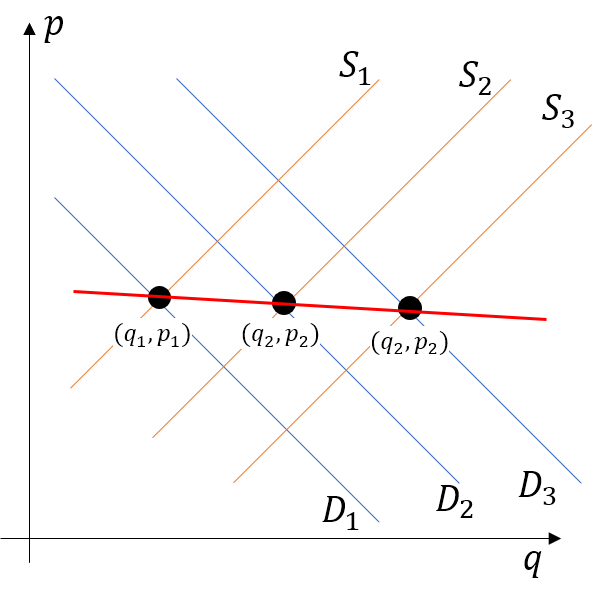
\includegraphics{fig_Demand_Supply.png}
\end{itemize}

\section{Idea of IV Regression}\label{idea-of-iv-regression}

\begin{itemize}
\item
  Let's start with a simple case. \[
  y_i = \beta_0 + \beta_1 x_i + \epsilon_i, 
  \] and \(Cov(x_i, \epsilon_i) \neq 0\).
\item
  Now, we consider another variable \(z_i\), which we call
  \textbf{instrumental variable (IV)}.
\item
  Instrumental variable \(z_i\) should satisfies the following two
  conditions:

  \begin{enumerate}
  \def\labelenumi{\arabic{enumi}.}
  \tightlist
  \item
    \textbf{Independence}: \(Cov(z_i, \epsilon_i) = 0\). No correlation
    between IV and error.
  \item
    \textbf{Relevance}: \(Cov(z_i, x_i) \neq 0\). There should be
    correlation between IV and endogenous variable \(x_i\).
  \end{enumerate}
\item
  Idea: Use the variation of \(x_i\) \textbf{induced by instrument
  \(z_i\)} to estimate the direct (causal) effect of \(x_i\) on \(y_i\),
  that is \(\beta_1\)!.
\item
  More on this:

  \begin{enumerate}
  \def\labelenumi{\arabic{enumi}.}
  \tightlist
  \item
    Intuitively, the OLS estimator captures the correlation between
    \(x\) and \(y\).
  \item
    If there is no correlation between \(x\) and \(\epsilon\), it
    captures the causal effect \(\beta_1\).
  \item
    If not, the OLS estimator captures both direct and indirect effect,
    the latter of which is bias.
  \item
    Now, let's capture the variation of \(x\) due to instrument \(z\),

    \begin{itemize}
    \tightlist
    \item
      Such a variation should exist under \textbf{relevance} assumption.
    \item
      Such a variation should not be correlated with the error under
      \textbf{independence assumption}
    \end{itemize}
  \item
    By looking at the correlation between such variation and \(y\), you
    can get the causal effect \(\beta_1\).
  \end{enumerate}
\end{itemize}

\begin{figure}
\centering
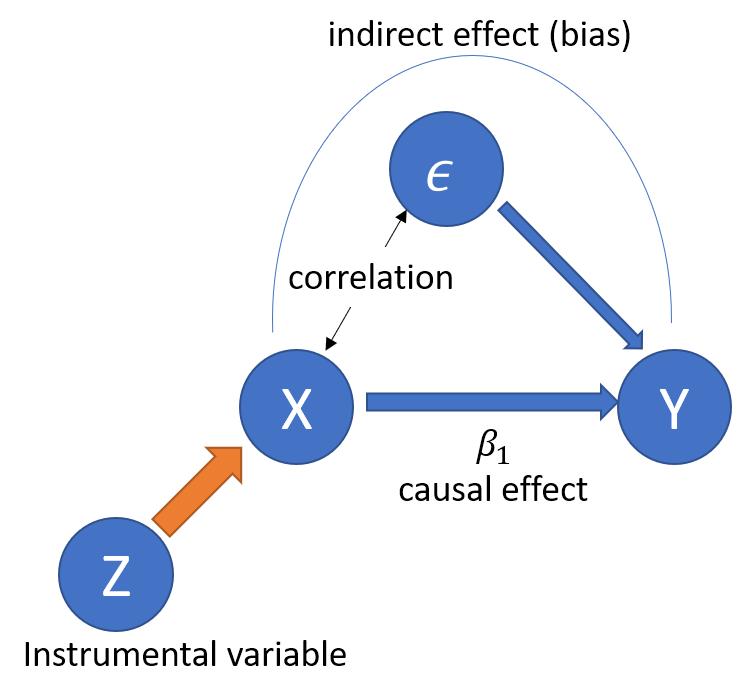
\includegraphics{fig_IV_idea.png}
\caption{Idea IV}
\end{figure}

\section{Formal Framework and
Estimation}\label{formal-framework-and-estimation}

\subsection{Model}\label{model}

\begin{itemize}
\tightlist
\item
  We now introduce a general framework with multiple endogenous
  variables and multiple instruments.
\item
  Consider the model \[
  \begin{aligned}
    Y_i = \beta_0 + \beta_1 X_{1i} + \dots + \beta_K X_{Ki} + \beta_{K+1} W_{1i} + \dots + \beta_{K+R} W_{Ri} + u_i, 
  \end{aligned}
  \] with \(i=1,\dots,n\) is the general instrumental variables
  regression model where

  \begin{itemize}
  \tightlist
  \item
    \(Y_i\) is the dependent variable
  \item
    \(\beta_0,\dots,\beta_{K+R}\) are \(1+K+R\) unknown regression
    coefficients
  \item
    \(X_{1i},\dots,X_{Ki}\) are \(K\) endogenous regressors:
    \(Cov(X_{ki}, u_i) \neq 0\) for all \(k\).
  \item
    \(W_{1i},\dots,W_{Ri}\) are \(R\) exogenous regressors which are
    uncorrelated with \(u_i\). \(Cov(W_{ri}, u_i) = 0\) for all \(r\).
  \item
    \(u_i\) is the error term
  \item
    \(Z_{1i},\dots,Z_{Mi}\) are \(M\) instrumental variables
  \end{itemize}
\item
  I will discuss conditions for valid instruments later.
\end{itemize}

\subsection{Estimation by Two Stage Least Squares
(2SLS)}\label{estimation-by-two-stage-least-squares-2sls}

\begin{itemize}
\tightlist
\item
  We can estimate the above model by \textbf{Two Stage Least Squares
  (2SLS)}
\item
  Step 1: \textbf{First-stage regression(s)}

  \begin{itemize}
  \tightlist
  \item
    Run an OLS regression for each of the endogenous variables
    (\(X_{1i},\dots,X_{ki}\)) on all instrumental variables
    (\(Z_{1i},\dots,Z_{mi}\)), all exogenous variables
    (\(W_{1i},\dots,W_{ri}\)) and an intercept.
  \item
    Compute the fitted values
    (\(\widehat{X}_{1i},\dots,\widehat{X}_{ki}\)).
  \end{itemize}
\item
  Step 2: \textbf{Second-stage regression}

  \begin{itemize}
  \tightlist
  \item
    Regress the dependent variable \(Y_i\) on \textbf{the predicted
    values} of all endogenous regressors
    (\(\widehat{X}_{1i},\dots,\widehat{X}_{ki}\)), all exogenous
    variables (\(W_{1i},\dots,W_{ri}\)) and an intercept using OLS.
  \item
    This gives
    \(\widehat{\beta}_{0}^{TSLS},\dots,\widehat{\beta}_{k+r}^{TSLS}\),
    the 2SLS estimates of the model coefficients.
  \end{itemize}
\end{itemize}

\subsubsection{Intuition}\label{intuition}

\begin{itemize}
\tightlist
\item
  Why does this work? Let's go back to the simple example with 1
  endogenous variable and 1 IV.
\item
  In the first stage, we estimate\\
  \[
  x_i = \pi_0 + \pi_1 z_i + v_i
  \] by OLS and obtain the fitted value
  \(\widehat{x}_i = \widehat{\pi}_0 + \widehat{\pi}_1 z_i\).
\item
  In the second stage, we estimate \[
  y_i = \beta_0 + \beta_1 \widehat{x}_i + u_i
  \]
\item
  Since \(\widehat{x}_i\) depends only on \(z_i\), which is uncorrelated
  with \(u_i\), the second stage can estimate \(\beta_1\) without bias.
\item
  Can you see the importance of both independence and relevance
  asssumption here? (More formal discussion later)
\end{itemize}

\subsection{Conditions for Valid IVs in a general
framework}\label{conditions-for-valid-ivs-in-a-general-framework}

\subsubsection{Necessary condition}\label{necessary-condition}

\begin{itemize}
\tightlist
\item
  Depending on the number of IVs, we have three cases

  \begin{enumerate}
  \def\labelenumi{\arabic{enumi}.}
  \tightlist
  \item
    Over-identification: \(M > K\)
  \item
    Just identification{]} \(M=K\)
  \item
    Under-identification \(M < K\)
  \end{enumerate}
\item
  The necessary condition is \(M \geq K\).

  \begin{itemize}
  \tightlist
  \item
    We should have more IVs than endogenous variables!!
  \end{itemize}
\end{itemize}

\subsubsection{Sufficient condition}\label{sufficient-condition}

\begin{itemize}
\tightlist
\item
  How about sufficiency?
\item
  In a general framework, the sufficient condition for valid instruments
  is given as follows.

  \begin{enumerate}
  \def\labelenumi{\arabic{enumi}.}
  \tightlist
  \item
    \textbf{Independence}: \(Cov( Z_{mi}, \epsilon_i) = 0\) for all
    \(m\).
  \item
    \textbf{Relevance}: In the second stage regression, the variables \[
    \left( \widehat{X}_{1i},\dots,\widehat{X}_{ki}, W_{1i},\dots,W_{ri}, 1 \right)
    \] are not perfectly multicollinear.
  \end{enumerate}
\item
  What does the relevance condition mean?
\item
  In the simple example above, The first stage is\\
  \[
  x_i = \pi_0 + \pi_1 z_i + v_i
  \] and the second stage is \[
  y_i = \beta_0 + \beta_1 \widehat{x}_i + u_i
  \]
\item
  The second stage would have perfect multicollinarity if \(\pi_1 = 0\)
  (i.e., \(\widehat{x}_i = \pi_0\)).
\item
  Back to the general case, the first stage for \(X_k\) can be written
  as \[
  X_{ki} = \pi_0 + \pi_1 Z_{1i} + \cdots + \pi_M Z_{Mi} + \pi_{M+1} W_{1i} + \cdots + \pi_{M+R} W_{Ri}
  \] and one of \(\pi_1 , \cdots, \pi_M\) should be non-zero.
\item
  Intuitively speaking, \textbf{the instruments should be correlated
  with endogenous variables after controlling for exogenous variables}
\end{itemize}

\section{Check Instrument Validity}\label{check-instrument-validity}

\subsection{Relevance}\label{relevance}

\begin{itemize}
\item
  Instruments are \textbf{weak} if those instruments explain little
  variation in the endogenous variables.
\item
  Weak instruments lead to

  \begin{enumerate}
  \def\labelenumi{\arabic{enumi}.}
  \tightlist
  \item
    imprecise estimates (higher standard errors)
  \item
    The asymptotic distribution would deviate from a normal distribution
    even if we have a large sample.
  \end{enumerate}
\item
  Here is a rule of thumb to check the relevance conditions.
\item
  Consider the case with one endogenous variable \(X_{1i}\).
\item
  The first stage regression\\
  \[
  X_k = \pi_0 + \pi_1 Z_{1i} + \cdots + \pi_M Z_{Mi} + \pi_{M+1} W_{1i} + \cdots + \pi_{M+R} W_{Ri}
  \]
\item
  And test the null hypothesis \[
  \begin{aligned}
  H_0 & : \pi_1 = \cdots = \pi_M = 0 \\ 
  H_1 & : otherwise
  \end{aligned}
  \]

  \begin{itemize}
  \tightlist
  \item
    This is F test (test of joint hypothesis)
  \end{itemize}
\item
  If we can reject this, we can say no concern for weak instruments.
\item
  A rule of thumbs is that the F statistic should be larger than 10.
\item ~
  \subsection{Independence (Instrument
  exogeneity)}\label{independence-instrument-exogeneity}
\item
  Arguing for independence is hard and a key in empirical analysis.
\item
  Justification of this assumption depends on a context, institutional
  features, etc\ldots{}
\item
  We will see this through examples in the next chapter.
\end{itemize}

\chapter{Instrumental Variable 2: Implementation in
R}\label{instrumental-variable-2-implementation-in-r}

\section{Example 1: Wage regression}\label{example-1-wage-regression}

\begin{itemize}
\tightlist
\item
  Use dataset ``Mroz'', cross-sectional labor force participation data
  that accompany ``Introductory Econometrics'' by Wooldridge.

  \begin{itemize}
  \tightlist
  \item
    Original data from \emph{``The Sensitivity of an Empirical Model of
    Married Women's Hours of Work to Economic and Statistical
    Assumptions''} by Thomas Mroz published in \emph{Econometrica} in
    1987.
  \item
    Detailed description of data:
    \url{https://www.rdocumentation.org/packages/npsf/versions/0.4.2/topics/mroz}
  \end{itemize}
\end{itemize}

\begin{Shaded}
\begin{Highlighting}[]
\KeywordTok{library}\NormalTok{(}\StringTok{"foreign"}\NormalTok{)}

\CommentTok{# You might get a message "cannot read factor labels from Stata 5 files", but you do not have to worry about it. }
\NormalTok{data <-}\StringTok{ }\KeywordTok{read.dta}\NormalTok{(}\StringTok{"MROZ.DTA"}\NormalTok{)}
\end{Highlighting}
\end{Shaded}

\begin{verbatim}
## Warning in read.dta("MROZ.DTA"): cannot read factor labels from Stata 5
## files
\end{verbatim}

\begin{itemize}
\tightlist
\item
  Describe data
\end{itemize}

\begin{Shaded}
\begin{Highlighting}[]
\KeywordTok{library}\NormalTok{(stargazer)}
\end{Highlighting}
\end{Shaded}

\begin{verbatim}
## 
## Please cite as:
\end{verbatim}

\begin{verbatim}
##  Hlavac, Marek (2018). stargazer: Well-Formatted Regression and Summary Statistics Tables.
\end{verbatim}

\begin{verbatim}
##  R package version 5.2.2. https://CRAN.R-project.org/package=stargazer
\end{verbatim}

\begin{Shaded}
\begin{Highlighting}[]
\KeywordTok{stargazer}\NormalTok{(data, }\DataTypeTok{type =} \StringTok{"text"}\NormalTok{)}
\end{Highlighting}
\end{Shaded}

\begin{verbatim}
## 
## ===================================================================
## Statistic  N     Mean     St. Dev.   Min   Pctl(25) Pctl(75)  Max  
## -------------------------------------------------------------------
## inlf      753   0.568      0.496      0       0        1       1   
## hours     753  740.576    871.314     0       0      1,516   4,950 
## kidslt6   753   0.238      0.524      0       0        0       3   
## kidsge6   753   1.353      1.320      0       0        2       8   
## age       753   42.538     8.073      30      36       49      60  
## educ      753   12.287     2.280      5       12       13      17  
## wage      428   4.178      3.310    0.128   2.263    4.971   25.000
## repwage   753   1.850      2.420    0.000   0.000    3.580   9.980 
## hushrs    753 2,267.271   595.567    175    1,928    2,553   5,010 
## husage    753   45.121     8.059      30      38       52      60  
## huseduc   753   12.491     3.021      3       11       15      17  
## huswage   753   7.482      4.231    0.412   4.788    9.167   40.509
## faminc    753 23,080.600 12,190.200 1,500   15,428   28,200  96,000
## mtr       753   0.679      0.083    0.442   0.622    0.721   0.942 
## motheduc  753   9.251      3.367      0       7        12      17  
## fatheduc  753   8.809      3.572      0       7        12      17  
## unem      753   8.624      3.115      3      7.5       11      14  
## city      753   0.643      0.480      0       0        1       1   
## exper     753   10.631     8.069      0       4        15      45  
## nwifeinc  753   20.129     11.635   -0.029  13.025   24.466  96.000
## lwage     428   1.190      0.723    -2.054  0.817    1.604   3.219 
## expersq   753  178.039    249.631     0       16      225    2,025 
## -------------------------------------------------------------------
\end{verbatim}

\begin{itemize}
\tightlist
\item
  Consider the wage regression \[
  \log(w_i) = \beta_0 + \beta_1 educ_i + \beta_2 exper_i + \beta_3 exper_i^2 + \epsilon_i
  \]
\item
  We assume that \(exper_i\) is exogenous but \(educ_i\) is endogenous.
\item
  As an instrument for \(educ_i\), we use the years of schooling for his
  or her father and mother, which we call \(fathereduc_i\) and
  \(mothereduc_i\).
\item
  Discussion on these IVs will be later.
\end{itemize}

\begin{Shaded}
\begin{Highlighting}[]
\KeywordTok{library}\NormalTok{(}\StringTok{"AER"}\NormalTok{)}
\end{Highlighting}
\end{Shaded}

\begin{verbatim}
##  要求されたパッケージ car をロード中です
\end{verbatim}

\begin{verbatim}
##  要求されたパッケージ carData をロード中です
\end{verbatim}

\begin{verbatim}
##  要求されたパッケージ lmtest をロード中です
\end{verbatim}

\begin{verbatim}
##  要求されたパッケージ zoo をロード中です
\end{verbatim}

\begin{verbatim}
## 
##  次のパッケージを付け加えます: 'zoo'
\end{verbatim}

\begin{verbatim}
##  以下のオブジェクトは 'package:base' からマスクされています: 
## 
##      as.Date, as.Date.numeric
\end{verbatim}

\begin{verbatim}
##  要求されたパッケージ sandwich をロード中です
\end{verbatim}

\begin{verbatim}
##  要求されたパッケージ survival をロード中です
\end{verbatim}

\begin{Shaded}
\begin{Highlighting}[]
\KeywordTok{library}\NormalTok{(}\StringTok{"dplyr"}\NormalTok{)}
\end{Highlighting}
\end{Shaded}

\begin{verbatim}
## 
##  次のパッケージを付け加えます: 'dplyr'
\end{verbatim}

\begin{verbatim}
##  以下のオブジェクトは 'package:car' からマスクされています: 
## 
##      recode
\end{verbatim}

\begin{verbatim}
##  以下のオブジェクトは 'package:stats' からマスクされています: 
## 
##      filter, lag
\end{verbatim}

\begin{verbatim}
##  以下のオブジェクトは 'package:base' からマスクされています: 
## 
##      intersect, setdiff, setequal, union
\end{verbatim}

\begin{Shaded}
\begin{Highlighting}[]
\CommentTok{# data cleaning}
\NormalTok{data }\OperatorTok\StringTok{ }
\StringTok{  }\KeywordTok{select}\NormalTok{(lwage, educ, exper, expersq, motheduc, fatheduc) }\OperatorTok
\StringTok{  }\KeywordTok{filter}\NormalTok{( }\KeywordTok{is.na}\NormalTok{(lwage) }\OperatorTok{==}\StringTok{ }\DecValTok{0}\NormalTok{ ) ->}\StringTok{ }\NormalTok{data}

\CommentTok{# OLS regression}
\NormalTok{result_OLS <-}\StringTok{ }\KeywordTok{lm}\NormalTok{( lwage }\OperatorTok{~}\StringTok{ }\NormalTok{educ }\OperatorTok{+}\StringTok{ }\NormalTok{exper }\OperatorTok{+}\StringTok{ }\NormalTok{expersq, }\DataTypeTok{data =}\NormalTok{ data)}

\CommentTok{# IV regression using fathereduc and mothereduc}
\NormalTok{result_IV <-}\StringTok{ }\KeywordTok{ivreg}\NormalTok{(lwage }\OperatorTok{~}\StringTok{ }\NormalTok{educ }\OperatorTok{+}\StringTok{ }\NormalTok{exper }\OperatorTok{+}\StringTok{ }\NormalTok{expersq }\OperatorTok{|}\StringTok{ }\NormalTok{fatheduc }\OperatorTok{+}\StringTok{ }\NormalTok{motheduc }\OperatorTok{+}\StringTok{ }\NormalTok{exper }\OperatorTok{+}\StringTok{ }\NormalTok{expersq, }\DataTypeTok{data =}\NormalTok{ data)}

\CommentTok{# Robust standard errors }
\CommentTok{# gather robust standard errors in a list}
\NormalTok{rob_se <-}\StringTok{ }\KeywordTok{list}\NormalTok{(}\KeywordTok{sqrt}\NormalTok{(}\KeywordTok{diag}\NormalTok{(}\KeywordTok{vcovHC}\NormalTok{(result_OLS, }\DataTypeTok{type =} \StringTok{"HC1"}\NormalTok{))),}
               \KeywordTok{sqrt}\NormalTok{(}\KeywordTok{diag}\NormalTok{(}\KeywordTok{vcovHC}\NormalTok{(result_IV, }\DataTypeTok{type =} \StringTok{"HC1"}\NormalTok{))))}

\CommentTok{# Show result}
\KeywordTok{stargazer}\NormalTok{(result_OLS, result_IV, }\DataTypeTok{type =}\StringTok{"text"}\NormalTok{, }\DataTypeTok{se =}\NormalTok{ rob_se)}
\end{Highlighting}
\end{Shaded}

\begin{verbatim}
## 
## ===================================================================
##                                        Dependent variable:         
##                                ------------------------------------
##                                               lwage                
##                                          OLS           instrumental
##                                                          variable  
##                                          (1)               (2)     
## -------------------------------------------------------------------
## educ                                  0.107***            0.061*   
##                                        (0.013)           (0.033)   
##                                                                    
## exper                                 0.042***           0.044***  
##                                        (0.015)           (0.016)   
##                                                                    
## expersq                                -0.001*           -0.001**  
##                                       (0.0004)           (0.0004)  
##                                                                    
## Constant                              -0.522***           0.048    
##                                        (0.202)           (0.430)   
##                                                                    
## -------------------------------------------------------------------
## Observations                             428               428     
## R2                                      0.157             0.136    
## Adjusted R2                             0.151             0.130    
## Residual Std. Error (df = 424)          0.666             0.675    
## F Statistic                    26.286*** (df = 3; 424)             
## ===================================================================
## Note:                                   *p<0.1; **p<0.05; ***p<0.01
\end{verbatim}

\begin{itemize}
\tightlist
\item
  How about the first stage? You should always check this!!
\end{itemize}

\begin{Shaded}
\begin{Highlighting}[]
\CommentTok{# First stage regression }

\NormalTok{result_1st <-}\StringTok{ }\KeywordTok{lm}\NormalTok{(educ }\OperatorTok{~}\StringTok{ }\NormalTok{motheduc }\OperatorTok{+}\StringTok{ }\NormalTok{fatheduc }\OperatorTok{+}\StringTok{ }\NormalTok{exper }\OperatorTok{+}\StringTok{ }\NormalTok{expersq, }\DataTypeTok{data =}\NormalTok{ data)}

\CommentTok{# F test}
\KeywordTok{linearHypothesis}\NormalTok{(result_1st, }
                 \KeywordTok{c}\NormalTok{(}\StringTok{"fatheduc = 0"}\NormalTok{, }\StringTok{"motheduc = 0"}\NormalTok{ ), }
                 \DataTypeTok{vcov =}\NormalTok{ vcovHC, }\DataTypeTok{type =} \StringTok{"HC1"}\NormalTok{)}
\end{Highlighting}
\end{Shaded}

\begin{verbatim}
## Linear hypothesis test
## 
## Hypothesis:
## fatheduc = 0
## motheduc = 0
## 
## Model 1: restricted model
## Model 2: educ ~ motheduc + fatheduc + exper + expersq
## 
## Note: Coefficient covariance matrix supplied.
## 
##   Res.Df Df      F                Pr(>F)    
## 1    425                                    
## 2    423  2 48.644 < 0.00000000000000022 ***
## ---
## Signif. codes:  0 '***' 0.001 '**' 0.01 '*' 0.05 '.' 0.1 ' ' 1
\end{verbatim}

\subsection{Discussion on IV}\label{discussion-on-iv}

\begin{itemize}
\tightlist
\item
  Labor economists have used family background variables as IVs for
  education.
\item
  Relevance: OK from the first stage regression.
\item
  Independence: A bit suspicious. Parents' education would be correlated
  with child's ability through quality of nurturing at an early age.
\item
  Still, we can see that these IVs can mitigate (though may not
  eliminate completely) the omitted variable bias.
\item
  Discussion on the validity of instruments is crucial in empirical
  research.
\end{itemize}

\section{Example 2: Estimation of the Demand for
Cigaretts}\label{example-2-estimation-of-the-demand-for-cigaretts}

\begin{itemize}
\item
  Demand model is a building block in many branches of Economics.
\item
  For example, health economics is concerned with the study of how
  health-affecting behavior of individuals is influenced by the
  health-care system and regulation policy.
\item
  Smoking is a prominent example as it is related to many illnesses and
  negative externalities.
\item
  It is plausible that cigarette consumption can be reduced by taxing
  cigarettes more heavily.
\item
  Question: how much taxes must be increased to reach a certain
  reduction in cigarette consumption? -\textgreater{} Need to know
  \textbf{price elasticity of demand} for cigaretts.
\item
  Use \texttt{CigarrettesSW} in the package \texttt{AER}.
\item
  a panel data set that contains observations on cigarette consumption
  and several economic indicators for all 48 continental federal states
  of the U.S. from 1985 to 1995.
\item
  What is \textbf{panel data}? The data involves both time series and
  cross-sectional information.

  \begin{itemize}
  \tightlist
  \item
    The variable is denoted as \(y_{it}\), which indexed by individual
    \(i\) and time \(t\).
  \item
    Cross section data \(y_i\): information for a particular individual
    \(i\) (e.g., income for person \(i\)).
  \item
    Time series data \(y_t\): information for a particular time period
    (e.g., GDP in year \(y\))
  \item
    Panel data \(y_{it}\): income of person \(i\) in year \(t\).
  \end{itemize}
\item
  We will see more on panel data later in this course. For now, we use
  the panel data as just cross-sectional data (\textbf{pooled
  cross-sections})
\end{itemize}

\begin{Shaded}
\begin{Highlighting}[]
\CommentTok{# load the data set and get an overview}
\KeywordTok{library}\NormalTok{(AER)}
\KeywordTok{data}\NormalTok{(}\StringTok{"CigarettesSW"}\NormalTok{)}
\KeywordTok{summary}\NormalTok{(CigarettesSW)}
\end{Highlighting}
\end{Shaded}

\begin{verbatim}
##      state      year         cpi          population      
##  AL     : 2   1985:48   Min.   :1.076   Min.   :  478447  
##  AR     : 2   1995:48   1st Qu.:1.076   1st Qu.: 1622606  
##  AZ     : 2             Median :1.300   Median : 3697472  
##  CA     : 2             Mean   :1.300   Mean   : 5168866  
##  CO     : 2             3rd Qu.:1.524   3rd Qu.: 5901500  
##  CT     : 2             Max.   :1.524   Max.   :31493524  
##  (Other):84                                               
##      packs            income               tax            price       
##  Min.   : 49.27   Min.   :  6887097   Min.   :18.00   Min.   : 84.97  
##  1st Qu.: 92.45   1st Qu.: 25520384   1st Qu.:31.00   1st Qu.:102.71  
##  Median :110.16   Median : 61661644   Median :37.00   Median :137.72  
##  Mean   :109.18   Mean   : 99878736   Mean   :42.68   Mean   :143.45  
##  3rd Qu.:123.52   3rd Qu.:127313964   3rd Qu.:50.88   3rd Qu.:176.15  
##  Max.   :197.99   Max.   :771470144   Max.   :99.00   Max.   :240.85  
##                                                                       
##       taxs       
##  Min.   : 21.27  
##  1st Qu.: 34.77  
##  Median : 41.05  
##  Mean   : 48.33  
##  3rd Qu.: 59.48  
##  Max.   :112.63  
## 
\end{verbatim}

\begin{itemize}
\tightlist
\item
  Consider the following model \[
  \log (Q_{it}) = \beta_0 + \beta_1 \log (P_{it}) + \beta_2 \log(income_{it}) + u_{it}
  \] where

  \begin{itemize}
  \tightlist
  \item
    \(Q_{it}\) is the number of packs per capita in state \(i\) in year
    \(t\),
  \item
    \(P_{it}\) is the after-tax average real price per pack of
    cigarettes, and
  \item
    \(income_{it}\) is the real income per capita. This is demand
    shifter.
  \end{itemize}
\item
  As an IV for the price, we use the followings:

  \begin{itemize}
  \tightlist
  \item
    \(SalesTax_{it}\): the proportion of taxes on cigarettes arising
    from the general sales tax.

    \begin{itemize}
    \tightlist
    \item
      Relevant as it is included in the after-tax price
    \item
      Exogenous(indepndent) since the sales tax does not influence
      demand directly, but indirectly through the price.
    \end{itemize}
  \item
    \(CigTax_{it}\): the cigarett-specific taxes
  \end{itemize}
\end{itemize}

\begin{Shaded}
\begin{Highlighting}[]
\KeywordTok{library}\NormalTok{(dplyr)}
\NormalTok{CigarettesSW }\OperatorTok\StringTok{ }
\StringTok{  }\KeywordTok{mutate}\NormalTok{( }\DataTypeTok{rincome =}\NormalTok{ (income }\OperatorTok{/}\StringTok{ }\NormalTok{population) }\OperatorTok{/}\StringTok{ }\NormalTok{cpi) }\OperatorTok\StringTok{ }
\StringTok{  }\KeywordTok{mutate}\NormalTok{( }\DataTypeTok{rprice  =}\NormalTok{ price }\OperatorTok{/}\StringTok{ }\NormalTok{cpi ) }\OperatorTok\StringTok{ }
\StringTok{  }\KeywordTok{mutate}\NormalTok{( }\DataTypeTok{salestax =}\NormalTok{ (taxs }\OperatorTok{-}\StringTok{ }\NormalTok{tax) }\OperatorTok{/}\StringTok{ }\NormalTok{cpi ) }\OperatorTok\StringTok{ }
\StringTok{  }\KeywordTok{mutate}\NormalTok{( }\DataTypeTok{cigtax =}\NormalTok{ tax}\OperatorTok{/}\NormalTok{cpi ) ->}\StringTok{ }\NormalTok{Cigdata}
\end{Highlighting}
\end{Shaded}

\begin{itemize}
\tightlist
\item
  Let's run the regressions
\end{itemize}

\begin{Shaded}
\begin{Highlighting}[]
\NormalTok{cig_ols <-}\StringTok{ }\KeywordTok{lm}\NormalTok{(}\KeywordTok{log}\NormalTok{(packs) }\OperatorTok{~}\StringTok{ }\KeywordTok{log}\NormalTok{(rprice) }\OperatorTok{+}\StringTok{ }\KeywordTok{log}\NormalTok{(rincome) ,  }\DataTypeTok{data =}\NormalTok{ Cigdata)}
\CommentTok{#coeftest(cig_ols, vcov = vcovHC, type = "HC1")}


\NormalTok{cig_ivreg <-}\StringTok{ }\KeywordTok{ivreg}\NormalTok{(}\KeywordTok{log}\NormalTok{(packs) }\OperatorTok{~}\StringTok{ }\KeywordTok{log}\NormalTok{(rprice) }\OperatorTok{+}\StringTok{ }\KeywordTok{log}\NormalTok{(rincome)  }\OperatorTok{|}\StringTok{ }
\StringTok{                    }\KeywordTok{log}\NormalTok{(rincome) }\OperatorTok{+}\StringTok{  }\NormalTok{salestax }\OperatorTok{+}\StringTok{  }\NormalTok{cigtax, }\DataTypeTok{data =}\NormalTok{ Cigdata)}
\CommentTok{#coeftest(cig_ivreg, vcov = vcovHC, type = "HC1")}

\CommentTok{# Robust standard errors }
\NormalTok{rob_se <-}\StringTok{ }\KeywordTok{list}\NormalTok{(}\KeywordTok{sqrt}\NormalTok{(}\KeywordTok{diag}\NormalTok{(}\KeywordTok{vcovHC}\NormalTok{(cig_ols, }\DataTypeTok{type =} \StringTok{"HC1"}\NormalTok{))),}
               \KeywordTok{sqrt}\NormalTok{(}\KeywordTok{diag}\NormalTok{(}\KeywordTok{vcovHC}\NormalTok{(cig_ivreg, }\DataTypeTok{type =} \StringTok{"HC1"}\NormalTok{))))}

\CommentTok{# Show result}
\KeywordTok{stargazer}\NormalTok{(cig_ols, cig_ivreg, }\DataTypeTok{type =}\StringTok{"text"}\NormalTok{, }\DataTypeTok{se =}\NormalTok{ rob_se)}
\end{Highlighting}
\end{Shaded}

\begin{verbatim}
## 
## =================================================================
##                                       Dependent variable:        
##                               -----------------------------------
##                                           log(packs)             
##                                        OLS           instrumental
##                                                        variable  
##                                        (1)               (2)     
## -----------------------------------------------------------------
## log(rprice)                         -1.334***         -1.229***  
##                                      (0.154)           (0.155)   
##                                                                  
## log(rincome)                         0.318**            0.257*   
##                                      (0.154)           (0.153)   
##                                                                  
## Constant                            10.067***          9.736***  
##                                      (0.502)           (0.514)   
##                                                                  
## -----------------------------------------------------------------
## Observations                            96                96     
## R2                                    0.552             0.549    
## Adjusted R2                           0.542             0.539    
## Residual Std. Error (df = 93)         0.165             0.165    
## F Statistic                   57.185*** (df = 2; 93)             
## =================================================================
## Note:                                 *p<0.1; **p<0.05; ***p<0.01
\end{verbatim}

\begin{itemize}
\tightlist
\item
  The first stage regression
\end{itemize}

\begin{Shaded}
\begin{Highlighting}[]
\CommentTok{# First stage regression }

\NormalTok{result_1st <-}\StringTok{ }\KeywordTok{lm}\NormalTok{(}\KeywordTok{log}\NormalTok{(rprice) }\OperatorTok{~}\StringTok{ }\KeywordTok{log}\NormalTok{(rincome) }\OperatorTok{+}\StringTok{ }\KeywordTok{log}\NormalTok{(rincome) }\OperatorTok{+}\StringTok{ }\NormalTok{salestax }\OperatorTok{+}\StringTok{ }\NormalTok{cigtax , }\DataTypeTok{data=}\NormalTok{ Cigdata)}

\CommentTok{# F test}
\KeywordTok{linearHypothesis}\NormalTok{(result_1st, }
                 \KeywordTok{c}\NormalTok{(}\StringTok{"salestax = 0"}\NormalTok{, }\StringTok{"cigtax = 0"}\NormalTok{ ), }
                 \DataTypeTok{vcov =}\NormalTok{ vcovHC, }\DataTypeTok{type =} \StringTok{"HC1"}\NormalTok{)}
\end{Highlighting}
\end{Shaded}

\begin{verbatim}
## Linear hypothesis test
## 
## Hypothesis:
## salestax = 0
## cigtax = 0
## 
## Model 1: restricted model
## Model 2: log(rprice) ~ log(rincome) + log(rincome) + salestax + cigtax
## 
## Note: Coefficient covariance matrix supplied.
## 
##   Res.Df Df      F                Pr(>F)    
## 1     94                                    
## 2     92  2 127.77 < 0.00000000000000022 ***
## ---
## Signif. codes:  0 '***' 0.001 '**' 0.01 '*' 0.05 '.' 0.1 ' ' 1
\end{verbatim}

\section{Example 3: Effects of Turnout on Partisan
Voting}\label{example-3-effects-of-turnout-on-partisan-voting}

\begin{itemize}
\tightlist
\item
  THOMAS G. HANSFORD and BRAD T. GOMEZ ``Estimating the Electoral
  Effects of Voter Turnout'' The American Political Science Review Vol.
  104, No. 2 (May 2010), pp.~268-288

  \begin{itemize}
  \tightlist
  \item
    Link:
    \url{https://www.cambridge.org/core/journals/american-political-science-review/article/estimating-the-electoral-effects-of-voter-turnout/8A880C28E79BE770A5CA1A9BB6CF933C}
  \end{itemize}
\item
  Here, we will see a simplified version of their analysis.
\item
  The dataset is \href{HansfordGomez_Data.csv}{here}
\end{itemize}

\begin{Shaded}
\begin{Highlighting}[]
\KeywordTok{library}\NormalTok{(readr)}
\end{Highlighting}
\end{Shaded}

\begin{verbatim}
## Warning: パッケージ 'readr' はバージョン 3.5.3 の R の下で造られました
\end{verbatim}

\begin{Shaded}
\begin{Highlighting}[]
\NormalTok{HGdata <-}\StringTok{ }\KeywordTok{read_csv}\NormalTok{(}\StringTok{"HansfordGomez_Data.csv"}\NormalTok{)}
\end{Highlighting}
\end{Shaded}

\begin{verbatim}
## Parsed with column specification:
## cols(
##   .default = col_double()
## )
\end{verbatim}

\begin{verbatim}
## See spec(...) for full column specifications.
\end{verbatim}

\begin{Shaded}
\begin{Highlighting}[]
\NormalTok{stargazer}\OperatorTok{::}\KeywordTok{stargazer}\NormalTok{(}\KeywordTok{as.data.frame}\NormalTok{(HGdata), }\DataTypeTok{type=}\StringTok{"text"}\NormalTok{)}
\end{Highlighting}
\end{Shaded}

\begin{verbatim}
## 
## =========================================================================================
## Statistic           N       Mean       St. Dev.      Min   Pctl(25)  Pctl(75)     Max    
## -----------------------------------------------------------------------------------------
## Year              27,401  1,973.972     16.111      1,948    1,960     1,988     2,000   
## FIPS_County       27,401 29,985.500   13,081.250    4,001   20,013    39,157     56,045  
## Turnout           27,401   65.562       10.514     20.366   58.477    72.613    100.000  
## Closing2          27,401   23.053       13.042        0       11        30        125    
## Literacy          27,401    0.058        0.234        0        0         0         1     
## PollTax           27,401    0.001        0.023        0        0         0         1     
## Motor             27,401    0.211        0.408        0        0         0         1     
## GubElection       27,401    0.434        0.496        0        0         1         1     
## SenElection       27,401    0.680        0.467        0        0         1         1     
## GOP_Inc           27,401    0.501        0.500        0        0         1         1     
## Yr52              27,401    0.071        0.258        0        0         0         1     
## Yr56              27,401    0.071        0.258        0        0         0         1     
## Yr60              27,401    0.071        0.258        0        0         0         1     
## Yr64              27,401    0.071        0.258        0        0         0         1     
## Yr68              27,401    0.071        0.258        0        0         0         1     
## Yr72              27,401    0.071        0.258        0        0         0         1     
## Yr76              27,401    0.071        0.258        0        0         0         1     
## Yr80              27,401    0.071        0.258        0        0         0         1     
## Yr84              27,401    0.072        0.258        0        0         0         1     
## Yr88              27,401    0.072        0.258        0        0         0         1     
## Yr92              27,401    0.072        0.258        0        0         0         1     
## Yr96              27,401    0.072        0.258        0        0         0         1     
## Yr2000            27,401    0.070        0.256        0        0         0         1     
## DNormPrcp_KRIG    27,401    0.005        0.208     -0.419   -0.093     0.001     2.627   
## GOPIT             27,401   33.282       34.066        0        0       66.3       100    
## DemVoteShare2_3MA 27,401   44.250       10.606     10.145   37.006    50.996     88.982  
## DemVoteShare2     27,401   43.622       12.415      6.420   34.954    51.858     97.669  
## RainGOPI          27,401    0.007        0.142       -0      -0.03       0         2     
## TO_DVS23MA        27,401  2,886.877     792.530    473.161 2,321.025 3,384.772 8,526.616 
## Rain_DVS23MA      27,401    0.355       10.188     -25.054  -4.019     0.028    144.257  
## dph               27,401    0.021        0.145        0        0         0         1     
## dvph              27,401    0.018        0.133        0        0         0         1     
## rph               27,401    0.025        0.155        0        0         0         1     
## rvph              27,401    0.025        0.155        0        0         0         1     
## state_del         27,401    0.037        0.187     -0.821   -0.090     0.172     0.619   
## dph_StateVAP      27,401 77,525.150   597,474.000     0        0         0     6,150,988 
## dvph_StateVAP     27,401 63,138.400   663,707.600     0        0         0     12,700,000
## rph_StateVAP      27,401 243,707.900 1,720,659.000    0        0         0     18,300,000
## rvph_StateVAP     27,401 142,166.500 1,071,445.000    0        0         0     12,800,000
## State_DVS_lag     27,401   46.896        8.317     22.035   40.767    52.197     80.872  
## State_DVS_lag2    27,401  2,268.381     786.199    485.533 1,661.934 2,724.515 6,540.244 
## -----------------------------------------------------------------------------------------
\end{verbatim}

\begin{itemize}
\tightlist
\item
  Data description:
\end{itemize}

\begin{longtable}[]{@{}ll@{}}
\toprule
\begin{minipage}[b]{0.05\columnwidth}\raggedright\strut
Name\strut
\end{minipage} & \begin{minipage}[b]{0.89\columnwidth}\raggedright\strut
Description\strut
\end{minipage}\tabularnewline
\midrule
\endhead
\begin{minipage}[t]{0.05\columnwidth}\raggedright\strut
Year\strut
\end{minipage} & \begin{minipage}[t]{0.89\columnwidth}\raggedright\strut
Election Year\strut
\end{minipage}\tabularnewline
\begin{minipage}[t]{0.05\columnwidth}\raggedright\strut
FIPS\_County\strut
\end{minipage} & \begin{minipage}[t]{0.89\columnwidth}\raggedright\strut
FIPS County Code\strut
\end{minipage}\tabularnewline
\begin{minipage}[t]{0.05\columnwidth}\raggedright\strut
Turnout\strut
\end{minipage} & \begin{minipage}[t]{0.89\columnwidth}\raggedright\strut
Turnout as Pcnt VAP\strut
\end{minipage}\tabularnewline
\begin{minipage}[t]{0.05\columnwidth}\raggedright\strut
Closing2\strut
\end{minipage} & \begin{minipage}[t]{0.89\columnwidth}\raggedright\strut
Days between registration closing date and election\strut
\end{minipage}\tabularnewline
\begin{minipage}[t]{0.05\columnwidth}\raggedright\strut
Literacy\strut
\end{minipage} & \begin{minipage}[t]{0.89\columnwidth}\raggedright\strut
Literacy Test\strut
\end{minipage}\tabularnewline
\begin{minipage}[t]{0.05\columnwidth}\raggedright\strut
PollTax\strut
\end{minipage} & \begin{minipage}[t]{0.89\columnwidth}\raggedright\strut
Poll Tax\strut
\end{minipage}\tabularnewline
\begin{minipage}[t]{0.05\columnwidth}\raggedright\strut
Motor\strut
\end{minipage} & \begin{minipage}[t]{0.89\columnwidth}\raggedright\strut
Motor Voter\strut
\end{minipage}\tabularnewline
\begin{minipage}[t]{0.05\columnwidth}\raggedright\strut
GubElection\strut
\end{minipage} & \begin{minipage}[t]{0.89\columnwidth}\raggedright\strut
Gubernatorial Election in State\strut
\end{minipage}\tabularnewline
\begin{minipage}[t]{0.05\columnwidth}\raggedright\strut
SenElection\strut
\end{minipage} & \begin{minipage}[t]{0.89\columnwidth}\raggedright\strut
U.S. Senate Election in State\strut
\end{minipage}\tabularnewline
\begin{minipage}[t]{0.05\columnwidth}\raggedright\strut
GOP\_Inc\strut
\end{minipage} & \begin{minipage}[t]{0.89\columnwidth}\raggedright\strut
Republican Incumbent\strut
\end{minipage}\tabularnewline
\begin{minipage}[t]{0.05\columnwidth}\raggedright\strut
Yr52\strut
\end{minipage} & \begin{minipage}[t]{0.89\columnwidth}\raggedright\strut
1952 Dummy\strut
\end{minipage}\tabularnewline
\begin{minipage}[t]{0.05\columnwidth}\raggedright\strut
Yr56\strut
\end{minipage} & \begin{minipage}[t]{0.89\columnwidth}\raggedright\strut
1956 Dummy\strut
\end{minipage}\tabularnewline
\begin{minipage}[t]{0.05\columnwidth}\raggedright\strut
Yr60\strut
\end{minipage} & \begin{minipage}[t]{0.89\columnwidth}\raggedright\strut
1960 Dummy\strut
\end{minipage}\tabularnewline
\begin{minipage}[t]{0.05\columnwidth}\raggedright\strut
Yr64\strut
\end{minipage} & \begin{minipage}[t]{0.89\columnwidth}\raggedright\strut
1964 Dummy\strut
\end{minipage}\tabularnewline
\begin{minipage}[t]{0.05\columnwidth}\raggedright\strut
Yr68\strut
\end{minipage} & \begin{minipage}[t]{0.89\columnwidth}\raggedright\strut
1968 Dummy\strut
\end{minipage}\tabularnewline
\begin{minipage}[t]{0.05\columnwidth}\raggedright\strut
Yr72\strut
\end{minipage} & \begin{minipage}[t]{0.89\columnwidth}\raggedright\strut
1972 Dummy\strut
\end{minipage}\tabularnewline
\begin{minipage}[t]{0.05\columnwidth}\raggedright\strut
Yr76\strut
\end{minipage} & \begin{minipage}[t]{0.89\columnwidth}\raggedright\strut
1976 Dummy\strut
\end{minipage}\tabularnewline
\begin{minipage}[t]{0.05\columnwidth}\raggedright\strut
Yr80\strut
\end{minipage} & \begin{minipage}[t]{0.89\columnwidth}\raggedright\strut
1980 Dummy\strut
\end{minipage}\tabularnewline
\begin{minipage}[t]{0.05\columnwidth}\raggedright\strut
Yr84\strut
\end{minipage} & \begin{minipage}[t]{0.89\columnwidth}\raggedright\strut
1984 Dummy\strut
\end{minipage}\tabularnewline
\begin{minipage}[t]{0.05\columnwidth}\raggedright\strut
Yr88\strut
\end{minipage} & \begin{minipage}[t]{0.89\columnwidth}\raggedright\strut
1988 Dummy\strut
\end{minipage}\tabularnewline
\begin{minipage}[t]{0.05\columnwidth}\raggedright\strut
Yr92\strut
\end{minipage} & \begin{minipage}[t]{0.89\columnwidth}\raggedright\strut
1992 Dummy\strut
\end{minipage}\tabularnewline
\begin{minipage}[t]{0.05\columnwidth}\raggedright\strut
Yr96\strut
\end{minipage} & \begin{minipage}[t]{0.89\columnwidth}\raggedright\strut
1996 Dummy\strut
\end{minipage}\tabularnewline
\begin{minipage}[t]{0.05\columnwidth}\raggedright\strut
Yr2000\strut
\end{minipage} & \begin{minipage}[t]{0.89\columnwidth}\raggedright\strut
2000 Dummy\strut
\end{minipage}\tabularnewline
\begin{minipage}[t]{0.05\columnwidth}\raggedright\strut
DNormPrcp\_KRIG\strut
\end{minipage} & \begin{minipage}[t]{0.89\columnwidth}\raggedright\strut
Election day rainfall - differenced from normal rain for the day\strut
\end{minipage}\tabularnewline
\begin{minipage}[t]{0.05\columnwidth}\raggedright\strut
GOPIT\strut
\end{minipage} & \begin{minipage}[t]{0.89\columnwidth}\raggedright\strut
Turnout x Republican Incumbent\strut
\end{minipage}\tabularnewline
\begin{minipage}[t]{0.05\columnwidth}\raggedright\strut
DemVoteShare2\textasciitilde{}A\strut
\end{minipage} & \begin{minipage}[t]{0.89\columnwidth}\raggedright\strut
Partisan composition measure = 3 election moving avg. of Dem Vote
Share\strut
\end{minipage}\tabularnewline
\begin{minipage}[t]{0.05\columnwidth}\raggedright\strut
DemVoteShare2\strut
\end{minipage} & \begin{minipage}[t]{0.89\columnwidth}\raggedright\strut
Democratic Pres Candidate's Vote Share\strut
\end{minipage}\tabularnewline
\begin{minipage}[t]{0.05\columnwidth}\raggedright\strut
RainGOPI\strut
\end{minipage} & \begin{minipage}[t]{0.89\columnwidth}\raggedright\strut
Rainfall measure x Republican Incumbent\strut
\end{minipage}\tabularnewline
\begin{minipage}[t]{0.05\columnwidth}\raggedright\strut
TO\_DVS23MA\strut
\end{minipage} & \begin{minipage}[t]{0.89\columnwidth}\raggedright\strut
Turnout x Partisan Composition measure\strut
\end{minipage}\tabularnewline
\begin{minipage}[t]{0.05\columnwidth}\raggedright\strut
Rain\_DVS23MA\strut
\end{minipage} & \begin{minipage}[t]{0.89\columnwidth}\raggedright\strut
Rainfall measure x Partisan composition measure\strut
\end{minipage}\tabularnewline
\begin{minipage}[t]{0.05\columnwidth}\raggedright\strut
dph\strut
\end{minipage} & \begin{minipage}[t]{0.89\columnwidth}\raggedright\strut
=1 if home state of Dem pres candidate\strut
\end{minipage}\tabularnewline
\begin{minipage}[t]{0.05\columnwidth}\raggedright\strut
dvph\strut
\end{minipage} & \begin{minipage}[t]{0.89\columnwidth}\raggedright\strut
=1 if home state of Dem vice pres candidate\strut
\end{minipage}\tabularnewline
\begin{minipage}[t]{0.05\columnwidth}\raggedright\strut
rph\strut
\end{minipage} & \begin{minipage}[t]{0.89\columnwidth}\raggedright\strut
=1 if home state of Rep pres candidate\strut
\end{minipage}\tabularnewline
\begin{minipage}[t]{0.05\columnwidth}\raggedright\strut
rvph\strut
\end{minipage} & \begin{minipage}[t]{0.89\columnwidth}\raggedright\strut
=1 if home state of Rep vice pres candidate\strut
\end{minipage}\tabularnewline
\begin{minipage}[t]{0.05\columnwidth}\raggedright\strut
state\_del\strut
\end{minipage} & \begin{minipage}[t]{0.89\columnwidth}\raggedright\strut
avg common space score for the House delegation\strut
\end{minipage}\tabularnewline
\begin{minipage}[t]{0.05\columnwidth}\raggedright\strut
dph\_StateVAP\strut
\end{minipage} & \begin{minipage}[t]{0.89\columnwidth}\raggedright\strut
= dph*State voting age population\strut
\end{minipage}\tabularnewline
\begin{minipage}[t]{0.05\columnwidth}\raggedright\strut
dvph\_StateVAP\strut
\end{minipage} & \begin{minipage}[t]{0.89\columnwidth}\raggedright\strut
= dvph*State voting age population\strut
\end{minipage}\tabularnewline
\begin{minipage}[t]{0.05\columnwidth}\raggedright\strut
rph\_StateVAP\strut
\end{minipage} & \begin{minipage}[t]{0.89\columnwidth}\raggedright\strut
= rph*State voting age population\strut
\end{minipage}\tabularnewline
\begin{minipage}[t]{0.05\columnwidth}\raggedright\strut
rvph\_StateVAP\strut
\end{minipage} & \begin{minipage}[t]{0.89\columnwidth}\raggedright\strut
= rvph*State voting age population\strut
\end{minipage}\tabularnewline
\begin{minipage}[t]{0.05\columnwidth}\raggedright\strut
State\_DVS\_lag\strut
\end{minipage} & \begin{minipage}[t]{0.89\columnwidth}\raggedright\strut
State-wide Dem vote share, lagged one election\strut
\end{minipage}\tabularnewline
\begin{minipage}[t]{0.05\columnwidth}\raggedright\strut
State\_DVS\_lag2\strut
\end{minipage} & \begin{minipage}[t]{0.89\columnwidth}\raggedright\strut
State\_DVS\_lag squared\strut
\end{minipage}\tabularnewline
\bottomrule
\end{longtable}

\begin{itemize}
\tightlist
\item
  Consider the following regression \[
  DemoShare_{it} = \beta_0 + \beta_1 Turnout_{it} + u_t + u_{it}
   \] where

  \begin{itemize}
  \tightlist
  \item
    \(Demoshare_{it}\): Two-party vote share for Democrat candidate in
    county \(i\) in the presidential election in year \(t\)
  \item
    \(Turnout_{it}\): Turnout rate in county \(i\) in the presidential
    election in year \(t\)
  \item
    \(u_t\): \textbf{Year fixed effects}. Time dummies for each
    presidential election year
  \end{itemize}
\item
  As an IV, we use the rainfall measure denoted by
  \texttt{DNormPrcp\_KRIG}
\end{itemize}

\begin{Shaded}
\begin{Highlighting}[]
\CommentTok{# You can do this, but it is tedious.}
\NormalTok{hg_ols <-}\StringTok{ }\KeywordTok{lm}\NormalTok{( DemVoteShare2 }\OperatorTok{~}\StringTok{ }\NormalTok{Turnout }\OperatorTok{+}\StringTok{ }\NormalTok{Yr52 }\OperatorTok{+}\StringTok{ }\NormalTok{Yr56 }\OperatorTok{+}\StringTok{ }\NormalTok{Yr60 }\OperatorTok{+}\StringTok{ }\NormalTok{Yr64 }\OperatorTok{+}\StringTok{ }\NormalTok{Yr68 }\OperatorTok{+}\StringTok{ }
\StringTok{                }\NormalTok{Yr72 }\OperatorTok{+}\StringTok{ }\NormalTok{Yr76 }\OperatorTok{+}\StringTok{ }\NormalTok{Yr80 }\OperatorTok{+}\StringTok{ }\NormalTok{Yr84 }\OperatorTok{+}\StringTok{ }\NormalTok{Yr88 }\OperatorTok{+}\StringTok{ }\NormalTok{Yr92 }\OperatorTok{+}\StringTok{ }\NormalTok{Yr96 }\OperatorTok{+}\StringTok{ }\NormalTok{Yr2000,  }\DataTypeTok{data =}\NormalTok{ HGdata)}
\CommentTok{#coeftest(hg_ols, vcov = vcovHC, type = "HC1")}

\CommentTok{# By using "factor(Year)" as an explanatory variable, the regression automatically incorporates the dummies for each value.}
\NormalTok{hg_ols <-}\StringTok{ }\KeywordTok{lm}\NormalTok{( DemVoteShare2 }\OperatorTok{~}\StringTok{ }\NormalTok{Turnout }\OperatorTok{+}\StringTok{ }\KeywordTok{factor}\NormalTok{(Year)   ,  }\DataTypeTok{data =}\NormalTok{ HGdata)}
\CommentTok{#coeftest(hg_ols, vcov = vcovHC, type = "HC1")}

\CommentTok{# Iv regression}
\NormalTok{hg_ivreg <-}\StringTok{ }\KeywordTok{ivreg}\NormalTok{( DemVoteShare2 }\OperatorTok{~}\StringTok{ }\NormalTok{Turnout }\OperatorTok{+}\StringTok{ }\KeywordTok{factor}\NormalTok{(Year) }\OperatorTok{|}\StringTok{ }
\StringTok{                    }\KeywordTok{factor}\NormalTok{(Year) }\OperatorTok{+}\StringTok{ }\NormalTok{DNormPrcp_KRIG, }\DataTypeTok{data =}\NormalTok{ HGdata)}
\CommentTok{#coeftest(hg_ivreg, vcov = vcovHC, type = "HC1")}

\CommentTok{# Robust standard errors }
\NormalTok{rob_se <-}\StringTok{ }\KeywordTok{list}\NormalTok{(}\KeywordTok{sqrt}\NormalTok{(}\KeywordTok{diag}\NormalTok{(}\KeywordTok{vcovHC}\NormalTok{(hg_ols, }\DataTypeTok{type =} \StringTok{"HC1"}\NormalTok{))),}
               \KeywordTok{sqrt}\NormalTok{(}\KeywordTok{diag}\NormalTok{(}\KeywordTok{vcovHC}\NormalTok{(hg_ivreg, }\DataTypeTok{type =} \StringTok{"HC1"}\NormalTok{))))}

\CommentTok{# Show result}
\KeywordTok{stargazer}\NormalTok{(hg_ols, hg_ivreg, }\DataTypeTok{type =}\StringTok{"text"}\NormalTok{, }\DataTypeTok{se =}\NormalTok{ rob_se)}
\end{Highlighting}
\end{Shaded}

\begin{verbatim}
## 
## =========================================================================
##                                            Dependent variable:           
##                                  ----------------------------------------
##                                               DemVoteShare2              
##                                              OLS             instrumental
##                                                                variable  
##                                              (1)                 (2)     
## -------------------------------------------------------------------------
## Turnout                                   -0.157***            0.363**   
##                                            (0.008)             (0.178)   
##                                                                          
## factor(Year)1952                         -10.215***           -15.832*** 
##                                            (0.374)             (1.987)   
##                                                                          
## factor(Year)1956                          -8.756***           -13.656*** 
##                                            (0.357)             (1.746)   
##                                                                          
## factor(Year)1960                          -3.862***           -11.094*** 
##                                            (0.351)             (2.531)   
##                                                                          
## factor(Year)1964                          10.851***            6.837***  
##                                            (0.337)             (1.441)   
##                                                                          
## factor(Year)1968                          -6.477***           -8.514***  
##                                            (0.356)             (0.811)   
##                                                                          
## factor(Year)1972                         -13.749***           -16.473*** 
##                                            (0.335)             (1.022)   
##                                                                          
## factor(Year)1976                           -0.367             -2.111***  
##                                            (0.337)             (0.715)   
##                                                                          
## factor(Year)1980                         -10.346***           -11.696*** 
##                                            (0.356)             (0.620)   
##                                                                          
## factor(Year)1984                         -13.134***           -13.515*** 
##                                            (0.352)             (0.404)   
##                                                                          
## factor(Year)1988                          -5.712***           -4.951***  
##                                            (0.349)             (0.447)   
##                                                                          
## factor(Year)1992                           -0.327              -1.008**  
##                                            (0.362)             (0.469)   
##                                                                          
## factor(Year)1996                          -1.193***             0.811    
##                                            (0.377)             (0.782)   
##                                                                          
## factor(Year)2000                          -9.013***           -8.130***  
##                                            (0.386)             (0.465)   
##                                                                          
## Constant                                  59.085***            26.910**  
##                                            (0.560)             (11.024)  
##                                                                          
## -------------------------------------------------------------------------
## Observations                               27,401               27,401   
## R2                                          0.281               0.130    
## Adjusted R2                                 0.280               0.130    
## Residual Std. Error (df = 27386)           10.533               11.582   
## F Statistic                      763.153*** (df = 14; 27386)             
## =========================================================================
## Note:                                         *p<0.1; **p<0.05; ***p<0.01
\end{verbatim}

\begin{Shaded}
\begin{Highlighting}[]
\CommentTok{# First stage regression }
\NormalTok{hg_1st <-}\StringTok{ }\KeywordTok{lm}\NormalTok{(Turnout }\OperatorTok{~}\StringTok{  }\KeywordTok{factor}\NormalTok{(Year) }\OperatorTok{+}\StringTok{ }\NormalTok{DNormPrcp_KRIG, }\DataTypeTok{data=}\NormalTok{ HGdata)}

\CommentTok{# F test}
\KeywordTok{linearHypothesis}\NormalTok{(hg_1st, }
                 \KeywordTok{c}\NormalTok{(}\StringTok{"DNormPrcp_KRIG = 0"}\NormalTok{ ), }
                 \DataTypeTok{vcov =}\NormalTok{ vcovHC, }\DataTypeTok{type =} \StringTok{"HC1"}\NormalTok{)}
\end{Highlighting}
\end{Shaded}

\begin{verbatim}
## Linear hypothesis test
## 
## Hypothesis:
## DNormPrcp_KRIG = 0
## 
## Model 1: restricted model
## Model 2: Turnout ~ factor(Year) + DNormPrcp_KRIG
## 
## Note: Coefficient covariance matrix supplied.
## 
##   Res.Df Df      F           Pr(>F)    
## 1  27387                               
## 2  27386  1 44.029 0.00000000003296 ***
## ---
## Signif. codes:  0 '***' 0.001 '**' 0.01 '*' 0.05 '.' 0.1 ' ' 1
\end{verbatim}

\begin{itemize}
\tightlist
\item
  We will see this paper more in excercise 4 (due on July 9th).
\end{itemize}

\chapter{Exercise 3 (Problem Set 4)}\label{exercise-3-problem-set-4}

\begin{itemize}
\tightlist
\item
  Due date: June 18th (Tue) 11pm.
\end{itemize}

\section{Rules}\label{rules-1}

\begin{itemize}
\tightlist
\item
  If you are enrolled in Japanese class (i.e., Wednesday 2nd), you can
  use both Japanese and English to write your answer.
\item
  Submit your solution through \texttt{CourseN@vi}.
\item
  \textbf{Important:} Submission format
\item
  If you use Rmarkdown, please compile your Rmarkdown file into either
  ``html'' or ``PDF'' file and submit \textbf{both} the compiled file
  and a Rmarkdown file.
\item
  If you do not use Rmarkdown, please submit the document file that
  contains your answer and R script file (.R file) \textbf{separately},
  that is, you submit \textbf{two files}.
\end{itemize}

\section{Question: Demand Estimation}\label{question-demand-estimation}

\begin{itemize}
\item
  You might want to refer \href{IV_Examples_190524.pdf}{the lecture
  note} in my other class where I covered the same topic.
\item
  We use the dataset from Stephen Ryan (2012) ``The Costs of
  Environmental Regulation in a Concentrated Industry'', Econometrica,
  Issue 3, 1019-1061, 2012
\item
  This is the data for Portland cement in the US. The data is panel for
  22 regions (roughly corresponding to the US state) from 1981 to 1999.
\item
  Ryan (2012) studies the effects of environmental regulation on dynamic
  competition among cement producers.
\item
  Graduate-level knowledge about econometrics and industrial
  organization is needed to understand the whole paper. Rather we focus
  on a part of his analysis, that is demand estimation.
\item
  The dataset is \href{cementDec2009.csv}{here}.
\item
  The original dataset contains many variable. Here, we pick a subset of
  the variable we use in the analysis.
\end{itemize}

\begin{Shaded}
\begin{Highlighting}[]
\KeywordTok{library}\NormalTok{(readr)}
\end{Highlighting}
\end{Shaded}

\begin{verbatim}
## Warning: パッケージ 'readr' はバージョン 3.5.3 の R の下で造られました
\end{verbatim}

\begin{Shaded}
\begin{Highlighting}[]
\KeywordTok{library}\NormalTok{(dplyr)}
\end{Highlighting}
\end{Shaded}

\begin{verbatim}
## 
##  次のパッケージを付け加えます: 'dplyr'
\end{verbatim}

\begin{verbatim}
##  以下のオブジェクトは 'package:stats' からマスクされています: 
## 
##      filter, lag
\end{verbatim}

\begin{verbatim}
##  以下のオブジェクトは 'package:base' からマスクされています: 
## 
##      intersect, setdiff, setequal, union
\end{verbatim}

\begin{Shaded}
\begin{Highlighting}[]
\KeywordTok{library}\NormalTok{(stargazer)}
\end{Highlighting}
\end{Shaded}

\begin{verbatim}
## 
## Please cite as:
\end{verbatim}

\begin{verbatim}
##  Hlavac, Marek (2018). stargazer: Well-Formatted Regression and Summary Statistics Tables.
\end{verbatim}

\begin{verbatim}
##  R package version 5.2.2. https://CRAN.R-project.org/package=stargazer
\end{verbatim}

\begin{Shaded}
\begin{Highlighting}[]
\NormalTok{RyanData <-}\StringTok{ }\NormalTok{readr}\OperatorTok{::}\KeywordTok{read_csv}\NormalTok{(}\StringTok{"cementDec2009.csv"}\NormalTok{)}
\end{Highlighting}
\end{Shaded}

\begin{verbatim}
## Parsed with column specification:
## cols(
##   .default = col_double(),
##   region = col_character()
## )
\end{verbatim}

\begin{verbatim}
## See spec(...) for full column specifications.
\end{verbatim}

\begin{Shaded}
\begin{Highlighting}[]
\NormalTok{RyanData }\OperatorTok\StringTok{ }
\StringTok{  }\NormalTok{dplyr}\OperatorTok{::}\KeywordTok{select}\NormalTok{(year, shipped, price, wage96, coal96, elec96, population, gas96) ->}\StringTok{ }\NormalTok{RyanData}

\NormalTok{stargazer}\OperatorTok{::}\KeywordTok{stargazer}\NormalTok{(}\KeywordTok{as.data.frame}\NormalTok{(RyanData), }\DataTypeTok{type =} \StringTok{"text"}\NormalTok{)}
\end{Highlighting}
\end{Shaded}

\begin{verbatim}
## 
## =====================================================================================
## Statistic   N       Mean        St. Dev.      Min    Pctl(25)    Pctl(75)     Max    
## -------------------------------------------------------------------------------------
## year       483   1,989.907        5.537      1,981     1,985      1,995      1,999   
## shipped    483   2,850.592      1,575.068     186     1,717.5    3,689.5     10,262  
## price      483     67.935        13.731     39.351    58.644      74.892    138.992  
## wage96     483     31.679         4.377     20.139    28.695      34.475     44.338  
## coal96     483     26.904         8.243     15.880    19.190      34.200     42.330  
## elec96     483     5.706          1.023      4.230     4.750      6.740      7.600   
## population 483 10,297,214.000 7,410,527.000 689,584 4,692,603.0 12,000,000 33,100,000
## gas96      483     6.263          2.266      3.701     5.041      6.810      24.304  
## -------------------------------------------------------------------------------------
\end{verbatim}

\begin{itemize}
\tightlist
\item
  The data description
\end{itemize}

\begin{longtable}[]{@{}ll@{}}
\toprule
\begin{minipage}[b]{0.05\columnwidth}\raggedright\strut
Name\strut
\end{minipage} & \begin{minipage}[b]{0.89\columnwidth}\raggedright\strut
Description\strut
\end{minipage}\tabularnewline
\midrule
\endhead
\begin{minipage}[t]{0.05\columnwidth}\raggedright\strut
shipped\strut
\end{minipage} & \begin{minipage}[t]{0.89\columnwidth}\raggedright\strut
Quantity of cement shipped (measured in thousands of tons per
year)\strut
\end{minipage}\tabularnewline
\begin{minipage}[t]{0.05\columnwidth}\raggedright\strut
price\strut
\end{minipage} & \begin{minipage}[t]{0.89\columnwidth}\raggedright\strut
Price (measured in dollars per ton).\strut
\end{minipage}\tabularnewline
\begin{minipage}[t]{0.05\columnwidth}\raggedright\strut
wage96\strut
\end{minipage} & \begin{minipage}[t]{0.89\columnwidth}\raggedright\strut
wage in dollars per hour for skilled manufacturing workers, and taken
from County Business Patterns\strut
\end{minipage}\tabularnewline
\begin{minipage}[t]{0.05\columnwidth}\raggedright\strut
coal96\strut
\end{minipage} & \begin{minipage}[t]{0.89\columnwidth}\raggedright\strut
Coal price (dollars per ton)\strut
\end{minipage}\tabularnewline
\begin{minipage}[t]{0.05\columnwidth}\raggedright\strut
elec96\strut
\end{minipage} & \begin{minipage}[t]{0.89\columnwidth}\raggedright\strut
electricity price (dollars per kilowatt hour for electricity)\strut
\end{minipage}\tabularnewline
\begin{minipage}[t]{0.05\columnwidth}\raggedright\strut
population\strut
\end{minipage} & \begin{minipage}[t]{0.89\columnwidth}\raggedright\strut
the total populations of the states covered by a regional market.\strut
\end{minipage}\tabularnewline
\begin{minipage}[t]{0.05\columnwidth}\raggedright\strut
gas96\strut
\end{minipage} & \begin{minipage}[t]{0.89\columnwidth}\raggedright\strut
Gas price (dollars per thousand cubic feet for gas.)\strut
\end{minipage}\tabularnewline
\bottomrule
\end{longtable}

\begin{itemize}
\tightlist
\item
  Note that all price are adjusted to 1996 constant dollars.
\end{itemize}

\subsection{Questions}\label{questions-1}

\begin{enumerate}
\def\labelenumi{\arabic{enumi}.}
\item
  Estimate the demand model for the following two specifications with
  and without instruments. \[
  \begin{aligned}
  \log(Q_{jt}) & = \beta_0 + \beta_1 \log(P_{jt}) + \epsilon_{it} \\ 
  \log(Q_{jt}) & = \beta_0 + \beta_1 \log(P_{jt}) + \beta_2 population_{it} + \epsilon_{it} 
  \end{aligned}
  \] where \(Q_{jt}\): quantity, \(P_{jt}\): price, \(population_{jt}\):
  population As an instrument for price, you use wage, coal price,
  electricity price, and gas price. The variable \(population_{jt}\) is
  treated as exogenous.
\item
  Discuss the results above. In particular, explain (1) the importance
  of adding population as a control variable, and (2) the difference
  between results with and without IVs.
\item
  Discuss the validity of those instruments.
\item
  Instead of log-log specification, consider the following linear
  specification (with population as a control variable) \[
  Q_{jt}  = \beta_0 + \beta_1 P_{jt} + \beta_2 population_{it} + \epsilon_{it}. 
  \] Estimate this specification using instruments. Do not forget
  checking the 1st stage.
\item
  The price elasticity of demand is defined as \[
  \frac{\partial Q_{jt}}{\partial P_{jt} } \frac{P_{jt}}{Q_{jt}} 
  \] If we use the log-log specification, the coefficient on the price
  is the elasticity and it is constant across markets and time. Using
  the estimation result with linear specification, calculate the price
  elasticity for each observation (i.e., market-year pair). Report the
  summary statistics of the price elasticity across markets and time.
  Compare the result with the one from log-log specification that
  includes population as a control variable.
\end{enumerate}


\end{document}
